\documentclass[%
	draft,%
	twoside,%
	openright,%
	titlepage,%
	fleqn,%
	numbers=noenddot,%
	headinclude,
	10pt,%
	a4paper,%
	BCOR5mm,%
	footinclude,%
	cleardoublepage=empty,%	
	abstract=false%
	]{scrreprt}
%%%%%%%%%%%%%%%%%%%%%%%
% Packages with options that might require adjustments
%%%%%%%%%%%%%%%%%%%%%%%
\usepackage[utf8]{inputenc}
\usepackage[greek,ngerman,english]{babel}
\usepackage[square,numbers,sort&compress]{natbib}%normal Bibliography
\usepackage{multirow}
\usepackage{threeparttable}
\usepackage[fleqn]{amsmath}
\usepackage{classicthesis-ldpkg}
\usepackage[dvipsnames]{xcolor} % needed by tikz, so loading it before
\usepackage{tikz}
	\usetikzlibrary{shapes,arrows,patterns}
\usepackage{pgfplots}
	%\usetikzlibrary{pgfplotsclickable} make plots clickable
\usepackage[version=3]{mhchem}
\usepackage[load-configurations=abbreviations,load-configurations=binary,detect-all]{siunitx}
	\DeclareSIUnit\Molar{\textsc{m}}
\usepackage{makeidx}
\usepackage[shadow]{todonotes}
\usepackage{pdfpages}
\usepackage{isotope}
\usepackage{xfrac}
\usepackage[groups]{svn-multi}
\usepackage[%
	eulerchapternumbers,%
	%drafting,
	pdfspacing,%
	subfig,%
	beramono,%
	eulermath,%
	parts]{classicthesis}
%\usepackage[margin=1.3in]{geometry}\usepackage{setspace}\doublespacing
%%%%%%%%%%%Watermark
%\usepackage[firstpage]{draftwatermark} % try firstpage as option
%	\SetWatermarkLightness{0.618}
%	\SetWatermarkScale{0.618}
%	\SetWatermarkText{Special Edition}
%%%%%%%%%%%Watermark
\usepackage[all]{hypcap}
%%%%%%%%%%%%%%%%%%%%%%%
% Re-usable information
%%%%%%%%%%%%%%%%%%%%%%%
\svnidlong
	{$HeadURL$}
	{$LastChangedDate$}
	{$LastChangedRevision$}
	{$LastChangedBy$}
\svnid{$Id$}
\svngroup{Thesis-Group}
\newcommand{\myTitle}{High resolution tomographic imaging of the alveolar region of the mammalian lung\xspace}
\newcommand{\myDegree}{A close look deep into the lung\xspace}
\newcommand{\myName}{David Haberth\"ur\xspace}
\newcommand{\myProf}{Prof.\ Dr.\ Johannes C.\ Schittny\xspace}
\newcommand{\myOtherProf}{Dr.\ Mauricio Reyes\xspace}
\newcommand{\mySupervisor}{Prof.\ Dr.\ Martin Frenz\xspace}
\newcommand{\myFaculty}{Faculty of Medicine\xspace}
\newcommand{\myDepartment}{Institute of Anatomy\xspace}
\newcommand{\myUni}{\protect{University of Bern}\xspace}
\newcommand{\myLocation}{Bern, Switzerland\xspace}
\newcommand{\myTime}{May 2010\xspace}
%%%%%%%%%%%%%%%%%%%%%%%
% Setup and Finetuning
%%%%%%%%%%%%%%%%%%%%%%%
\newcommand{\imsize}{\linewidth}
\newlength{\abcd} % for ab..z string length calculation
\newcommand{\myfloatalign}{\centering} % how all the floats will be aligned
\newlength\imagewidth % needed for scalebars
\newlength\imagescale % ditto
\newcommand{\subfigureautorefname}{\figureautorefname} % to have subfigures named using \autoref
%%%%%%%%%%%%%%%%%%%%%%%
% Color (Re-Definition)
%%%%%%%%%%%%%%%%%%%%%%%
% according to http://is.gd/aOVVy
\definecolor{Maroon}{RGB}{229,5,58} % redefine Maroon to unibe (Pantone 192, RGB 229,5,58)
\definecolor{unibe-link}{RGB}{147,183,209} % define unibe-color for links (Pantone 543, RGB 147,183,209)
\definecolor{unibe-citation}{RGB}{216,140,2} % define unibe-color for citations (Pantone 138, RGB 216,140,2)
%%%%%%%%%%%%%%%%%%%%%%%
% Captions look and feel
%%%%%%%%%%%%%%%%%%%%%%%
\captionsetup{format=hang,font=small}
%%%%%%%%%%%%%%%%%%%%%%%
% Hyperreferences
%%%%%%%%%%%%%%%%%%%%%%%
\hypersetup{% http://www.jkrieger.de/tools/latex/hyperref.html helps!
	colorlinks=true, linktocpage=true, pdfstartpage=3, pdfstartview=FitV,%
	% uncomment the following line for black links for printing
	colorlinks=false, linktocpage=false, pdfborder={0 0 0}, pdfstartpage=3, pdfstartview=FitV,%
	breaklinks=true, pdfpagemode=UseNone, pageanchor=true, pdfpagemode=UseOutlines,%
	plainpages=false, bookmarksnumbered, bookmarksopen=true, bookmarksopenlevel=1,%
	hypertexnames=true, pdfhighlight=/O,%
	urlcolor=Maroon, linkcolor=unibe-link, citecolor=unibe-citation,%
	pdftitle={\myTitle},%
	pdfauthor={\myName, \myUni, \myFaculty},%
	pdfsubject={},%
	pdfkeywords={},%
	pdfcreator={pdfLaTeX},%
	pdfproducer={LaTeX with hyperref and classicthesis}%
	}
%%%%%%%%%%%%%%%%%%%%%%%
% GO!GO!GO! MOVE IT!
%%%%%%%%%%%%%%%%%%%%%%%
\begin{document}
\raggedbottom
\selectlanguage{english} % english and ngerman are set up by babel
\pagenumbering{roman}
\pagestyle{plain}
%%%%%%%%%%%%%%%%%%%%%%%
% Frontmatter
%%%%%%%%%%%%%%%%%%%%%%%
% !TEX root = ../Thesis.tex
%*******************************************************
% Little Dirty Titlepage
%*******************************************************
\thispagestyle{empty}
%\pdfbookmark[1]{Titel}{title}
%*******************************************************
\begin{center}
    \spacedlowsmallcaps{\myName} \\ \medskip                        

    \begingroup
        \color{Maroon}\spacedallcaps{\myTitle}
    \endgroup
\end{center}        

\cleardoublepage% !TEX root = ../Thesis.tex
%*******************************************************
% Titlepage
%*******************************************************
\begin{titlepage}
	\begin{addmargin}[-1cm]{-3cm}
    \begin{center}
        \large  

        \vfill

		\begingroup
			\color{Maroon}\spacedallcaps{\myTitle} \\ \bigskip
		\endgroup
		\myDegree \\
		\bigskip
		Graduate School for Cellular and Biomedical Sciences\\
		\myUni\\
		Ph.D.\ Thesis 

		\vfill

		%
\includegraphics[width=6cm]{gfx/TFZsuperellipse_bw} \\ \medskip

		Submitted by\\
		\medskip
		\spacedallcaps{\myName}\\
		\medskip
		from Metzerlen-Mariastein, SO\\

		\vfill

		Thesis Advisor\\
		\medskip
		\myProf \\
		\myDepartment \\                            
       	\myFaculty \\
       	\myUni \\
		\bigskip
       	\myTime                 
    \end{center}  
  \end{addmargin}       
\end{titlepage}   
% !TEX root = ../Thesis.tex
\thispagestyle{empty}
\hfill
\vfill

\noindent\myName\\\mbox{\emph{\myTitle}}\\\myDegree\\\myVersion
\bigskip

\noindent\spacedlowsmallcaps{Supervisors}:\\
\myProf \\
\myOtherProf \\ 
\mySupervisor
\medskip

\noindent\spacedlowsmallcaps{Location}:\\
\noindent\myLocation
\medskip

\noindent\spacedlowsmallcaps{Time Frame}:\\
September 2006--\myTime
\cleardoublepage% !TEX root = ../Thesis.tex
\thispagestyle{empty}
\hfill\vfill
\noindent Accepted by the Faculty of Medicine, the Faculty of Science and the Vetsuisse Faculty of the University of Bern at the request of the Graduate School for Cellular and Biomedical Sciences.

\vspace{2.5cm}
\noindent Bern,\hfill Dean of the Faculty of Medicine

\vspace{2.5cm}
\noindent Bern,\hfill Dean of the Faculty of Science

\vspace{2.5cm}
\noindent Bern,\hfill Dean of the Vetsuisse Faculty Bern\\
\cleardoublepage% !TEX root = ../Thesis.tex
%*******************************************************
% Dedication
%*******************************************************
\thispagestyle{empty}
%\phantomsection 
\refstepcounter{dummy}
\pdfbookmark[1]{Dedication}{Dedication}

\vspace*{7cm}

\begin{flushright}
    Dedicated to everyone who shared a path on my journey to this point.
\end{flushright}
\cleardoublepage% !TEX root = ../Thesis.tex
\pdfbookmark[1]{Abstract}{Abstract}%
\begingroup%
\let\clearpage\relax%
\let\cleardoublepage\relax%
\let\cleardoublepage\relax%
\chapter*{Abstract}%
Studying lung development in all its characteristics, especially analyzing the structural parameters of the terminal airways needs a fully three-dimensional imaging modality, since not all structural parameters can be assessed on classic histological sections.

Using synchrotron radiation based tomographic microscopy three-dimensional volumetric information of arbitrary samples can be obtained. The distinct advantages offered by tomographic microscopy make it an extremely well suited imaging method for the minute analysis of lung samples in three dimensions. Tomographic microscopy permits to study the samples in a non-destructive way and allows the acquisition of tomographic datasets with ultra high resolution in the micrometer scale in a short time, usually within a few minutes.

This work presents several methods for the analysis of the terminal airway using high resolution tomographic datasets. Using a combination of this imaging modality with transmission electron microscopy data we localized the deposition sites of sub-micrometer sized particles in the terminal airways and studied their properties.

Three-dimensional tomographic reconstructions were used for the analysis of structural parameters of the terminal airways. The achieved results confirmed the usability of tomographic data for confirming structural parameters obtained from classic histological slices, which highlights the advantage of the non-destructive scanning method.

The third method presented in this work makes it possible to record tomographic dataset of large\graffito{In the context of this work \emph{large} means with a volume of several cubic millimeters.} sample volumes with ultra high resolution. Using such datasets, we analyzed structural changes of the terminal airways of the mammalian lung during postnatal lung development. The presented method achieves a breakthrough for tomographic imaging, since generally a large field of view had to be traded for a high resolution, which is no longer necessary with the application of the so-called wide field scanning.
\endgroup%
\cleardoublepage% !TEX root = ../Thesis.tex
%*******************************************************
% Abstract
%*******************************************************
%\renewcommand{\abstractname}{Abstract}
\pdfbookmark[1]{Abstract}{Abstract}%
\begingroup%
\let\clearpage\relax%
\let\cleardoublepage\relax%
\let\cleardoublepage\relax%
\selectlanguage{ngerman}%
\pdfbookmark[1]{Zusammenfassung}{Zusammenfassung}%
\chapter*{Zusammenfassung}
Um die Lungenentwicklung, im speziellen die strukturellen Parameter der terminalen Luftwege detailliert analysieren zu können, muss ein dreidimensionales Abbildungsverfahren genutzt werden. Mit tomographische Röntgenmikroskopie basierend auf Synchrotronstrahlung können solche dreidimensionalen volumetrische Informationen von praktisch beliebigen Proben gewonnen werden. Die tomographische Mikroskopie bietet verschiedene Vorzüge, die sie zu einer bestens geeigneten Methode machen um Lungenproben minuziös in drei Dimensionen zu untersuchen; namentlich können die Proben zerstörungsfrei untersucht werden sowie bieten die resultierenden Daten höchste Auflösungen im Mikrometerbereich und können in wenigen Minuten aufgenommen werden.

Die vorliegende Arbeit präsentiert mehrere Methoden, um die terminalen Luftwege der Lunge mittels höchstaufgelösten tomographischen Daten zu untersuchen. Durch eine Kombination dieser Daten mit Elektronenmikroskopiebildern haben wir Partikel, welche kleiner als ein Mikrometer waren in den terminalen Luftwegen lokalisiert und konnten ihre Eigenschaften genau untersuchen.

Weiter haben wir dreidimensionale Rekonstruktionen von tomographischen Daten benutzt, um die struturellen Parameter der terminalen Luftwege zu untersuchen. Die Vergleich der erlangten Resultate mit Resultaten von klassischen Histologieschnitten zeigt, dass diese strukturellen Parameter genausogut auf tomographischen Daten erhoben werden können, ohne die Genauigkeit einzuschränken. Dies hebt den Vorteil der zerstörungsfreien tomographischen Abbildungsmethode hervor.

Die dritte Methode, welche in dieser Arbeit präsentiert wird, ermöglicht es, tomographische Datensätze von grossen\graffito{Gross heisst in diesem Zusammenhang mehrere Kubikmillimeter.} Lungenvolumina in höchster Auflösung aufzunehmen. So aufgenommene Datensätze ermöglichen es, Strukturänderungen der terminalen Luftwege in der Säugetierlunge zu untersuchen. Das vorgestellte Verfahren stellt einen Durchbruch in der tomographischen Mikroskopie dar, denn bis jetzt ging eine Vergrösserung der abgebildeten Volumina immer mit einer Verkleinerung der Auflösung der erzielten Daten einher\graffito{Mami, chunnsch no drus?}.
\selectlanguage{english}%
\endgroup%
\cleardoublepage% !TEX root = ../Thesis.tex
\acresetall
\pdfbookmark[1]{Acknowledgments}{acknowledgments}
\begin{flushright}{\slshape I'm throwing rocks tonight. Mark it, Dude.} \\ \medskip
    --- Steve Buscemi as Donny in\defcitealias{TheBigLebowski}{The Big Lebowski}\citetalias{TheBigLebowski} \citep{TheBigLebowski}
\end{flushright}
\vspace{6cm}

\begingroup
\let\clearpage\relax
\let\cleardoublepage\relax
\let\cleardoublepage\relax
\chapter*{Acknowledgments}
I thank Prof.\ Dr.\ Johannes C.\ Schittny for giving me the opportunity to carry out this work at the Institute of Anatomy at the University of Bern. Johannes introduced me into the delicate details of lung morphology, physiology and development and also provided multiple enjoyable moments away from the lab routine. Dr.\ Miguel Gonzàlez helped me to get on track with various image processing intricacies and was---after his  change from the \href{http://www.istb.unibe.ch/}{\ac{istb}} in Bern to \href{http://www.alma3d.com/en}{Alma IT Systems} in Spain---very well substituted by Dr.\ Mauricio Reyes from the \ac{istb}, which watched over the second half of my time working for this thesis. Both Miguel and Mauricio deserve thanks for their guidance as co-referees of this work. Prof.\ Dr.\ Martin Frenz acted as my mentor for the Graduate School for Cellular and Biomedical Sciences of the University of Bern. Already during my Master Thesis I had the pleasure to work under the guidance of  Martin and I am thankful for his watching eye as a mentor on this work.

Both Sébastien Barré and Lilian Salm shared the office with me during the last months at the Institute of Anatomy and contributed to the pleasant atmosphere in our group. Sébastien was a helpful discussion partner for all MATLAB problems and countless hours trying to stay awake and alert during numerous beamtime shifts at \acs{tomcat}. Lilian spent many kyphotic\graffito{She's a med student, she knows what kyphotic means\ldots} hours counting alveolar bridges with the STEPanizer and is responsible for the nice counting results shown in the discussion. Mohammed Ouanella was an expert help with the preparation of the samples and also provided excellent food from his home country, Algeria. Thanks!

The whole staff at the Institute of Anatomy provided for a great time; special thanks go to Dr.\ Stefan Tschanz for unconditional help with all things IT and for putting up with my special wishes concerning the use of the computing infrastructure here at the institute. Chrigu Lehmann had to put up with lathe machining \SI{0.6}{\milli\meter} Epon samples before we switched to paraffin embedded ``big'' lung samples and always provided generous help with special mechanical tasks for our need or for not work-related stuff like a riveting a broken buckle back to my ski boots. Our secretary team and especially Therese Dudan always provided the first friendly smiles in the morning when I came in to pick up our mail.

Special thanks go to the whole team at the \acs{tomcat} beamline at the \acl{sls} of the \acl{psi} in Villigen. Prof.\ Dr.\ Marco F.\ M.\ Stampanoni, head of the \acs{tomcat} beamline at the \acl{sls} and assistant Professor for X-ray Microscopy at the Department for Information Technology and Electrical Engineering of the ETH in Zürich provided a pleasurable work environment and was an invaluable resource on all things tomography and x-rays, provided well founded critique for my work and helped me to brush up my Italian skills both written and spoken. Dr.\ Christoph Hintermüller was not only a great guidance during my Master Thesis for the postgraduate course in Medical Physics but provided expert support at the beamline and countless interesting discussions, both scientific and completely non-scientific. Xris' insight into scripting, UNIX commands and image processing was a great help. Without the work of Dr.\ Federica Marone on the tomographic reconstruction algorithms and implementation of those algorithms at the beamline most of the wide-field-scan tomographic reconstructions in this work would not exist.

The University sports Berne, the Velokurier Bern and Fabio Breil with the eccentric bike provided me with athletic balance to the time spent at the desk in front of my monitors.

My friends Pesche, Bruni, Wöufu, Sigi and Nicola as well as Mara and Barbara provided (sometimes much needed) diversion from the academic turf and shared loads of lunch times. Dan and Tobi as (former) flatmates also helped to wrap my brain around different stuff than academics. Thanks!

Without my family I would not be where I am today. Mom, Dad and Nina, I'll always
be grateful to all of you.

Nina\graffito{Note that both my sister and girlfriend share the same first name, but are different persons. Nonetheless, both Ninas helped a great deal with the proof-reading of this work.} Hostettlers love makes me happy. I love you!
\endgroup
\pagestyle{scrheadings}
\cleardoublepage% !TEX root = ../Thesis.tex
%*******************************************************
% Table of Contents
%*******************************************************
%\phantomsection
\refstepcounter{dummy}
\pdfbookmark[1]{\contentsname}{tableofcontents}
\setcounter{tocdepth}{2} % <-- 2 includes up to subsections in the ToC
\setcounter{secnumdepth}{3} % <-- 3 numbers up to subsubsections
\manualmark
\markboth{\spacedlowsmallcaps{\contentsname}}{\spacedlowsmallcaps{\contentsname}}
\tableofcontents 
\automark[section]{chapter}
\renewcommand{\chaptermark}[1]{\markboth{\spacedlowsmallcaps{#1}}{\spacedlowsmallcaps{#1}}}
\renewcommand{\sectionmark}[1]{\markright{\thesection\enspace\spacedlowsmallcaps{#1}}}
%*******************************************************
% List of Figures and of the Tables
%*******************************************************
\clearpage

\begingroup 
    \let\clearpage\relax
    \let\cleardoublepage\relax
    \let\cleardoublepage\relax
    %*******************************************************
    % List of Figures
    %*******************************************************    
    %\phantomsection 
    \refstepcounter{dummy}
    %\addcontentsline{toc}{chapter}{\listfigurename}
    \pdfbookmark[1]{\listfigurename}{lof}
    \listoffigures

    \vspace*{8ex}

    %*******************************************************
    % List of Tables
    %*******************************************************
    %\phantomsection 
    \refstepcounter{dummy}
    %\addcontentsline{toc}{chapter}{\listtablename}
    \pdfbookmark[1]{\listtablename}{lot}
    \listoftables
        
    \vspace*{8ex}
	%\newpage
    
	%*******************************************************
	% List of Listings
	%*******************************************************      
	%\phantomsection 
%	\refstepcounter{dummy}
    %\addcontentsline{toc}{chapter}{\lstlistlistingname}
%    \pdfbookmark[1]{\lstlistlistingname}{lol}
%    \lstlistoflistings 
%    \vspace*{8ex}
	\newpage

    %*******************************************************
    % Acronyms
    %*******************************************************
    %\phantomsection
    \refstepcounter{dummy}
    \pdfbookmark[1]{Acronyms}{acronyms}
    \markboth{\spacedlowsmallcaps{Acronyms}}{\spacedlowsmallcaps{Acronyms}}
    \chapter*{Acronyms}
	\begin{acronym}[WF-SRXTM]
		\acro{amd}[AMD]{Advanced Micro Devices, Inc.}
		\acro{avv}[AVV]{I have no idea what an \acsu{avv} is, but it's used in a Monty Python sketch\ldots}
		\acro{bp}[BP]{Blood Pressure}
		\acro{cad}[CAD]{Computer Aided Design}
		\acro{ccd}[CCD]{Charge-Coupled Device}
		\acro{cfd}[CFD]{Computational Fluid Dynamics}
		\acro{ct}[CT]{Computed Tomography}
		\acro{cpu}[CPU]{Central Processing Unit}
		\acro{dat}[DAT]{Proprietary file format for \acs{fe} analysis}
		\acro{dcmm}[DCMM]{Double Crystal Multilayer Monochromator}
		\acro{eeg}[EEG]{Electroencephalography}: Using an \acsu{eeg}, the electrical activity of the brain can be measured.
		\acro{epics}[EPICS]{Experimental Physics and Industrial Control System}: Control system by the national laboratory of \href{http://www.aps.anl.gov/epics/}{Argonne in the USA}, used to control \acs{tomcat}.
		\acro{em}[EM]{Electron Microscopy}: An electron microscope produces an electronically magnified image of a specimen for detailed observation. The electron microscope uses an electron beam to illuminate the specimen and create a magnified image of it.
		\acro{fe}[FE]{Finite Element}
		\acro{fft}[FFT]{Fast Fourier Transform}
		\acro{gbha}[GBHA]{Grid-Based Hexahedral Algorithm}
		\acro{istb}[ISTB]{Institute for Surgical Technology \& Biomechanics}
		\acro{lm}[LM]{Light microscopy}
		\acro{lst}[LST]{Laplacian Smoothing Technique}
		\acro{uct}[\micro CT]{micro-Computed Tomography}
		\acro{mri}[MRI]{Magnetic Resonance Imaging}
		\acro{oca}[OCA]{Object Connectivity Analysis}
		\acro{oln}[OLN]{Object Label Number}
		\acro{pc}[PC]{Personal Computer}
		\acro{psi}[PSI]{Paul Scherrer Institut}: The \acs{psi} is the largest research centre for natural and engineering sciences in Switzerland.
		\acro{ram}[RAM]{Random-Access Memory}
		\acro{roi}[ROI]{Region of Interest}
		\acro{se}[SE]{Standard Error}: Standard deviation of a sample normalized by the square root of the sample size.
		\acro{tem}[TEM]{Transmission Electron Microscopy}: \acs{tem} is a microscopy  technique whereby a beam of electrons is transmitted through an very thin specimen.
		\acro{tomcat}[TOMCAT]{TOmographic Microscopy and Coherent rAdiology experimenTs}: \acs{tomcat} is the beamline at the \acs{sls}, where all experiments of this thesis have been performed.
		\acro{sem}[SEM]{Scanning Electron Microscopy}: \acs{sem} is an electron microscopy technique that images the sample surface by scanning it with a high-energy beam of electrons in a raster scan pattern.
		\acro{sls}[SLS]{Swiss Light Source}: The \acs{sls} at the \acs{psi} is a third-generation synchrotron light source.
		\acro{snr}[SNR]{Signal-to-Noise Ratio}
		\acro{sr}[SR]{Synchrotron Radiation}
		\acro{srct}[SRCT]{Synchrotron Radiation Computed Tomography}
		\acro{srxtm}[SRXTM]{Synchrotron Radiation based X-ray Tomographic Microscopy}
		\acro{stl}[STL]{Surface Tessellation or Standard Triangulation Language or Standard Tessellation Language}: A file format used as a Quasi-Standard of many \acs{cad}-systems.
		\acro{vrml}[VRML]{Virtual Reality Modeling Language}
		\acro{wf-srxtm}[WF-SRXTM]{Wide Field Synchrotron Radiation Based X-ray Tomographic Microscopy}: The method to increase the field of view of tomographic imaging stations presented in \autoref{ch:haberthuer2010}.
		\acro{xml}[XML]{Extensible Markup Language}: A set of rules for electronic encoding of documents.
		\acro{yag}[YAG]{Yttrium Aluminium Garnet}
	\end{acronym}
\endgroup

\cleardoublepage
%%%%%%%%%%%%%%%%%%%%%%%
% Mainmatter
%%%%%%%%%%%%%%%%%%%%%%%
\pagenumbering{arabic}
\cleardoublepage\myPart{Introduction}\label{part:introduction}
% !TEX root = ../Thesis.tex
\myChapter{Introduction}\label{ch:Introduction}
\begin{flushright}{\slshape    
		It's a magical world, Hobbes, ol' buddy\dots\\
		\dots Let's go exploring!}\\ \medskip
		--- Calvin, by\defcitealias{Watterson1996}{Bill Watterson}\citetalias{Watterson1996} \citep{Watterson1996}
\end{flushright}
\bigskip

Seeing and observing the object of interest has alwas been a crucial part of medical and biological research. If not by the naked eye, the object has been studied with ever-increasing resolution. In biomedical reasearch, state of the art imaging methods include light and electron microscopy\todo{Referenzen}. Even higher resolutions, down to \SI{10}{\nano\meter} \todo{how much?} can be reached with x-ray microscopy.

\section{High resolution imaging}
One of the main problems with light and electron microscopy is the destructive sample preparation. For both methods, the sample has to be sectioned in thin slices\todo{wie dünn genau?}. This process destroys the three-dimensional structure of the sample and makes is very time consuming to reconstruct the three-dimensional placement of the slices to extract the structural information. \citet{Woodward2005}~\todo{Moar?} have shown that a three-dimensional reconstruction of parts of the gas exchanging region of the avian lung is feasible, but the process is both extremely timeconsuming and needs very precise registration of the stack of slices cut from the sample. An exception to the destructive sample preparation is offered by confocal microscopy\todo{Citation?}. In confocal microscopy, light originating from outside the focal plane is excluded using a spatial pinhole. This allows for the definition of a section through a sample thicker than the optical focal plane of the objective. By positioning the focal plane stepwise through the whole sample, the three-dimensional information of the sample can be obtained. This method obviously only works with translucent samples.

In contrast to this, tomographic imaging makes it possible to non-destructively study the three-dimensional structure of a wide variety of samples. Two-dimensional projections of the sample can be taken fairly easily using a multitude of methods (e.g.\ X-Ray, light, Infrared\todo{true?}). These two-dimensional images include partical three-dimensional infomration fo the sample volume which has been transversted in the projection. If several projection images are acquired from different directions through the sample, the full three-dimensional infromation can be obtained. Using computed tomography\todo{cite Hounsfield}, a three-dimensional representation of the sample can be reconstructed and obtained. The theory and concepts behind the tomographic reconstruction are explained in more depth in chapter~\ref{ch:ct}.

\begin{itemize}
	\item Why the Mammalian lung?
	\item see chapter~\ref{ch:lung}
\end{itemize}

\section{Outline of the Thesis}
Main goal of the PhD-Thesis.

This thesis is structured into three parts:
\begin{description}
	\item[Part I] contains this introduction and gives a short overview over the lung development in chapter~\ref{ch:lung}. Chapter~\ref{ch:ct} explains the most important concepts in computed tomography and gives a short description of the \acf{TOMCAT} beamline, where all high resolution tomography experiments of this work have been performed.
	\item[Part II] contains publications written during the time of my Ph.D.\ Thesis at the Institute of Anatomy. Chapter~\ref{ch:XRM2008} consists of a proceeding written for the 9\textsuperscript{th} \href{http://xrm2008.web.psi.ch/}{InternatioTnal Conference on X-Ray Microscopy} in Zürich, Switzerland, from the 21\textsuperscript{st} to the 25\textsuperscript{th} July 2008. This proceeding describes a method to precisely localise instilled sub-micron sized gold particles in rat lungs through a combination of high resolution synchrotron radiation tomographic microscopy and \acl{TEM}.

Chapter~\ref{ch:Tsuda2008} consists of a paper submitted to the \href{http://jap.physiology.org/}{Journal of Applied Physiology} in which a new image processing method for accurate three dimensional reconstruction of the gas exchange region of the lung. This method is based on a finite element analysis of datasets obtained with high resolution synchrotron radiation tomographic microscopy.

Chapter~\ref{ch:Haberthuer2010} presents a method to increase the field of view of synchrotron radiation tomographic microscopy while keeping the advantage of a high resolution, something which is generally not possible with such an increase in the field of view. Additionally---through optimization of the acquisition protocol---the radiation dose inflicted on the sample can be greatly reduced.

	\item[Part III] contains two chapters with an overview over the obtained results and an outlook on further work based on this thesis.
\end{description}
% !TEX root = ../Thesis.tex
\acresetall
\myChapter{The mammalian lung}\label{ch:lung}
\begin{flushright}{\slshape If we're gonna move forward, this is the next logical step!} \\ \medskip
	--- Kevin Bacon\\as Sebastian in\defcitealias{HollowMan}{The Hollow Man}\citetalias{HollowMan} \citep{HollowMan}
\end{flushright}
\vspace{6cm}

The lung is, in relation to the surface one of the largest mammalian organs. It has the second biggest inner surface after the intestinal tract, which has a size of approximately \SI{320}{\meter\squared}~\cite{Takahashi1999}, the skin being distant third with approximately \SI{2}{\meter\squared}~\cite{Haycock1978}\graffito{Keep in mind that, \href{http://is.gd/bLoaZ}{that the measured length of area depends on the scale of measurement}, as first described by \citet{Richardson1961} and popularized by \citet{Mandelbrot1967}.}. Both organs are involved in the uptake of the most important, vital substances like oxygen, water and sugar. The function of the lung is essential for the transport of oxygen from the air we breathe into the blood and for the transport of carbon dioxide from biological processes out of the blood stream back into the atmosphere.


The lung can fulfill its function through its design, which is specifically optimized to provide a large gas exchange surface---in humans an area equivalent to about $\sfrac{3}{4}$ of a tennis court, \SI{130}{\meter\squared}~\cite{Weibel2009}---where capillary blood efficiently gets in close contact to the air inside the lung structure. The large area maximizes the region where the oxygen uptake can take place and a very thin tissue barrier maximizes the diffusion of the oxygen into the blood stream.

\section{Lung Development}
During lung development all the internal structures like the conducting airways, the blood vessel network and the gas exchange area are formed. 

Mammalian lung development can be divided into five overlapping stages~\cite{Schittny2004,Schittny2007a}, which are shown in the gray region in \autoref{fig:lung development stages old}: Organogenesis starts with a outpouching of the foregut resulting in the appearance of the lung buds and formation of the major airways. Subsequently, the conducting airways and parts of the respiratory airways are formed by a successive cycle of branching and growth starting at the lung buds, which is called branching morphogenesis. Most of this process takes place during the first lung development stage, the pseudoglandular stage. In this stage the functional respiratory lung unit, the so-called acinus is formed. An acinus is defined as the complex of alveolated airways distal of a last purely conducting airway, the terminal bronchiole~\cite{Rodriguez1987}. The total of all acini forms the lung parenchyma, the area where the pulmonary gas-exchange takes place.

\begin{figure}[htb]
	\noindent\makebox[\textwidth]{%
		\centering%
		%\documentclass{article}
%\usepackage{tikz,pgfplots}
%\usepackage[graphics,tightpage,active]{preview}
%\PreviewEnvironment{tikzpicture}
%\begin{document}
%%%%%%%%%%%%%%%%%%%%%%%%%%%%%%%%%%%%%%%%%%%%%%%%%%%%%%%%%%%%%%
	\pgfplotsset{width=\linewidth,height=.5\linewidth}
	\begin{tikzpicture}
		\def\xmin{4}
		\def\xmax{85}
		\def\ymin{0}
		\def\ymax{0.4}
		\begin{axis}[xbar stacked,%
			scale only axis,%
			xmin=\xmin,%
			xmax=\xmax,%
			ymin=\ymin,%
			ymax=\ymax,%
			yticklabels={},%
			axis x discontinuity=crunch,%
			xtick={9,...,\xmax},%
			xticklabels={},
			xlabel=Days,%
			axis y line=none]
		\end{axis}
		\begin{axis}[xbar stacked,%
			scale only axis,%
			xmin=\xmin,%
			xmax=\xmax,%
			ymin=\ymin,%
			ymax=\ymax,%
			yticklabels={},%
			axis x discontinuity=crunch,%
			xtick={11,13,18.5,20,21,25,35,42,57,81},%
			xticklabels={11,,,,Birth,4,14,21,36,60},
			xmajorgrids,%
			xlabel=Days,%
			%axis x line=bottom,%
			axis y line=none]
			\def\step{0.05}
			%\node [font=\footnotesize] at (axis cs:42,0.35) {X};
			%\node [font=\footnotesize] at (axis cs:85,0.35) {X};
			%\node [font=\footnotesize] at (axis cs:63.5,0.35) {Lung Growth (4 weeks--adulthood)};
			\addplot [transparent]	coordinates {(11,0)};
			\addplot [fill=red]		coordinates {(2,1*\step)};
			\addplot [fill=cyan]		coordinates {(5.5,2*\step)};
			\addplot [fill=blue]		coordinates {(1.5,3*\step)};
			\addplot [fill=magenta]	coordinates {(5,4*\step)};
			\addplot [fill=yellow]	coordinates {(10,5*\step)};
			\addplot [fill=orange]	coordinates {(7,6*\step)};
			\addplot [fill=green]		coordinates {(\xmax-41,7*\step)};

			\tikzstyle{every pin}=[%
				%fill=white,%
				%semitransparent,%
				%draw=black,%
				%text width=10em,%
				font=\footnotesize,
				%text centered,%
				pin distance=3ex]
			\node[coordinate, pin=right:{Embrionic Period (E11--E13)}] at (axis cs:13,0.05) {};
			\node[coordinate, pin=right:{Pseudoglandular Stage (E13--E18.5)}] at (axis cs:18.5,0.1) {};
			\node[coordinate, pin=right:{Canalicular Stage (E18.5--E20)}] at (axis cs:20,0.15) {};
			\node[coordinate, pin=right:{Saccular Stage (E20--P4)}] at (axis cs:25,0.2) {};
			\node[coordinate, pin=right:{Alveolarization (P4--P14)}] at (axis cs:35,0.25) {};
			\node[coordinate, pin=right:{Microvascular maturation (P14--P21)}] at (axis cs:42,0.3) {};
			\node[coordinate, pin=left:{Lung Growth (4 weeks--adulthood)}] at (axis cs:42,0.35) {};
		\end{axis}
	\end{tikzpicture}%
%%%%%%%%%%%%%%%%%%%%%%%%%%%%%%%%%%%%%%%%%%%%%%%%%%%%%%%%%%%%%%
%\end{document}%
		}%
	\caption[Lung development stages]{Lung development stages for the rat lung according to the currently valid paradigm. The first three stages (Embryonic Period, Pseudoglandular and Canalicular Stage) take place in the approximately 21 days from the beginning of gestation to birth. E=embryonic day (days post-coitus), D=postnatal day. The five stages mentioned in the text happen during the grey marked period. Note that the microvascular maturation and lung growth stages overlap each other by several days. All the other stages are drawn consecutively, but in reality they do slightly overlap, since as biological processes they change into each other. Figure adapted from~\cite{Schittny2007a}.}
	\label{fig:lung development stages old}
\end{figure}

The pseudoglandular stage is followed by intermediate stages, which are called canalicular and saccular. During the canalicular stage a first functional gas exchange surface---the air-blood barrier---is formed and the lung epithelium starts to differentiate. The saccular stage marks the switch from branching to septation morphogenesis.

During the alveolar stage the distal part of the bronchial tree is enlarged by the introduction of new alveoli through a formation of additional septa from already existing septa. 

After bulk alveolarization is completed, the interalveolar septa and their capillary networks are remodeled during the phase of microvascular maturation in order to optimize gas exchange. At this point lung development is considered to be finished and normal growth of the organ follows\graffito{The time point of birth differs between mammals, relative to the state of lung development. In humans, birth happens at the beginning of the alveolarization stage.}.

It was believed that lung developments comes to completion during the early postnatal period due to the reduction of a double- to a single-layered capillary network inside the alveolar septa. After this period, only growth of the organ should follow, and no additional alveolar septa are introduced in the lung parenchyma~\cite{Burri1999,Schittny2004}. \citet{Schittny2008} were able to refine this model with an additional development stage in which the so called late alveolarization---the formation of alveolar septa until young adulthood (days 4--60 in rats)---takes place. A local duplication of the capillary network was detected as the basis of these newly forming septa. \autoref{fig:lung development stages new} shows the refined sequence of the lung development stages. Two alveolarization phases and the phase of microvascular maturation occur simultaneously after postnatal day four until postnatal day 60.

\begin{figure}[htb]
	\noindent\makebox[\textwidth]{%
		\centering%
		% !TEX root = ../Thesis.tex
%\documentclass{article}
%\usepackage{tikz,pgfplots}
%\usepackage[graphics,tightpage,active]{preview}
%\PreviewEnvironment{tikzpicture}
%\begin{document}
%%%%%%%%%%%%%%%%%%%%%%%%%%%%%%%%%%%%%%%%%%%%%%%%%%%%%%%%%%%%%%
	\pgfplotsset{width=\linewidth,height=.5\linewidth}
	\begin{tikzpicture}
		\def\xmin{4}
		\def\xmax{85}
		\def\ymin{0}
		\def\ymax{0.4}
		\begin{axis}[xbar stacked,%
			scale only axis,%
			xmin=\xmin,%
			xmax=\xmax,%
			ymin=\ymin,%
			ymax=\ymax,%
			yticklabels={},%
			axis x discontinuity=crunch,%
			xtick={9,...,\xmax},%
			xticklabels={},
			xlabel=Days,%
			axis y line=none]
		\end{axis}
		\begin{axis}[xbar stacked,%
			scale only axis,%
			xmin=\xmin,%
			xmax=\xmax,%
			ymin=\ymin,%
			ymax=\ymax,%
			yticklabels={},%
			axis x discontinuity=crunch,%
			xtick={11,13,18.5,20,21,25,35,42,57,81},%
			xticklabels={11,,,,Birth,4,14,21,36,$\sim$60},
			xmajorgrids,%
			xlabel=Days,%
			%axis x line=bottom,%
			axis y line=none]
			%\node [font=\footnotesize] at (axis cs:25,0.25) {X};
			%\node [font=\footnotesize] at (axis cs:81,0.25) {X};
			\node [font=\footnotesize] at (axis cs:53,0.25) {First \& second phase of Alveolarization (P4--P60)};
			\node [font=\footnotesize] at (axis cs:53,0.3) {Microvascular Maturation (P4--P60)};
			\def\step{0.05}
			\addplot [transparent]	coordinates {(11,0)};
			\addplot [fill=red]		coordinates {(2,1*\step)};
			\addplot [fill=cyan]		coordinates {(5.5,2*\step)};
			\addplot [fill=blue]		coordinates {(1.5,3*\step)};
			\addplot [fill=magenta]	coordinates {(5,4*\step)};
			\addplot [fill=yellow]	coordinates {(56,5*\step)};
			\addplot [transparent]	coordinates {(-56,5.5*\step)};
			\addplot [fill=orange]	coordinates {(56,6*\step)};
			\addplot [transparent]	coordinates {(-5,5.5*\step)};
			\addplot [fill=green]		coordinates {(\xmax-75,7*\step)};
			\tikzstyle{every pin}=[%
				%fill=white,%
				%semitransparent,%
				%draw=black,%
				%text width=10em,%
				font=\footnotesize,
				%text centered,%
				pin distance=3ex]
			\node[coordinate, pin=right:{Embrionic Period (E11--E13)}] at (axis cs:13,0.05) {};
			\node[coordinate, pin=right:{Pseudoglandular Stage (E13--E18.5)}] at (axis cs:18.5,0.1) {};
			\node[coordinate, pin=right:{Canalicular Stage (E18.5--E20)}] at (axis cs:20,0.15) {};
			\node[coordinate, pin=right:{Saccular Stage (E20--P4)}] at (axis cs:25,0.2) {};
			\node[coordinate, pin=left:{Lung Growth (P60--adulthood)}] at (axis cs:76,0.35) {};
		\end{axis}
	\end{tikzpicture}%
%%%%%%%%%%%%%%%%%%%%%%%%%%%%%%%%%%%%%%%%%%%%%%%%%%%%%%%%%%%%%%
%\end{document}%
		}%
	\caption[Lung development stages]{Lung development stages with concurrently occurring Alveolarization and Microvascular Maturation stages. E=embryonic day (days post-coitus), D=postnatal day. Note that the alveolarization, microvascular maturation and lung growth stages overlap each other. Data for days $>$60 has not been recorded. Unpublished data from private communication with Johannes C.\ Schittny.}
	\label{fig:lung development stages new}
\end{figure}

\section{The functional units of the lung}
The airway structure of the mammalian lung is formed from dichotomous branches, starting from the trachea. The first branching generations lead into the bronchi (\autoref{subfig:lung diagram}). With increasing depth into the airway tree, the diameter of the airways is reduced, the bronchi are divided into bronchioles, leading to the terminal bronchioles which mark the end of the purely conducting airways. The respiratory bronchioles mark the start of the gas-exchange region in the lung, the point from which the so-called acinar airways and the acinus begin. 

Ongoing from the respiratory bronchioles, the acinus is further subdivided into alveolar ducts, sacculi and alveoli, as shown in \autoref{subfig:lung units}~\cite{Haefeli-Bleuer1988,Weibel1963,Weibel2009,Schittny2007a}. Note that \autoref{subfig:lung units} shows a representation of the generations in the human lung. Instead of several generations of respiratory bronchioles as in the human lung, rat lungs only have one generation of transitory bronchioles.

\renewcommand{\imsize}{0.55\linewidth}
\begin{figure}[htb]%
	\centering%
	\subfloat[]{%
		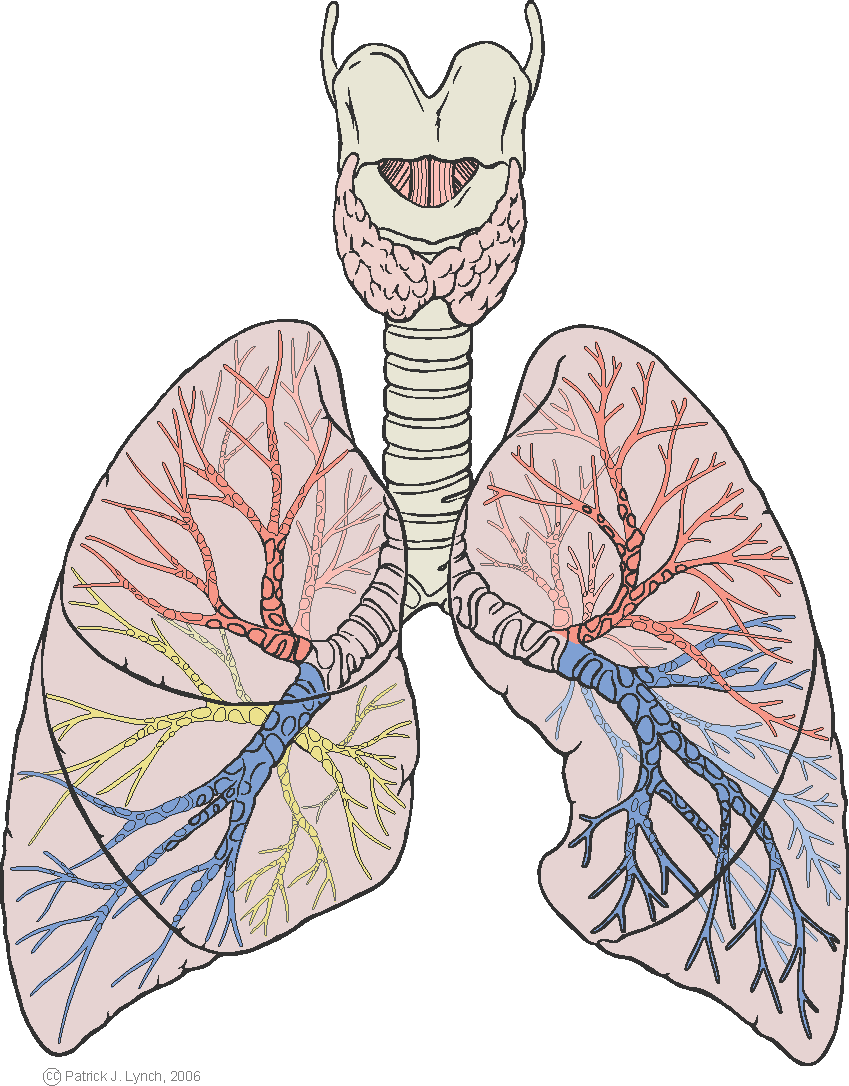
\includegraphics[width=\imsize]{img/Lungs_diagram_detailed}%
		\label{subfig:lung diagram}%
		}%
		\hfill%
	\subfloat[]{%
		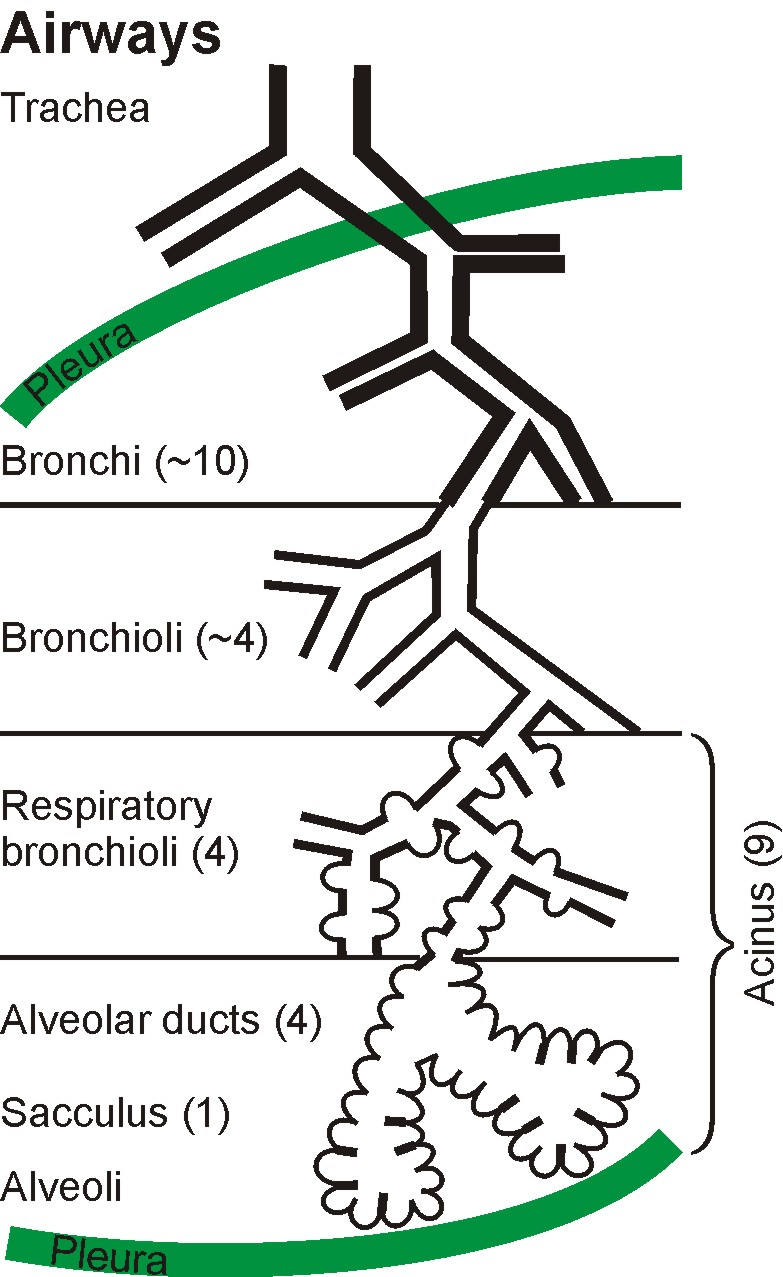
\includegraphics[height=0.7031\linewidth]{img/Lungunits}%
		\label{subfig:lung units}%
		}%
	\caption[Details of the human lung]{Details of the human lung. \subref{subfig:lung diagram}: Lung diagram of the human lung. From \cite{LungDiagram}. \subref{subfig:lung units}: Airway generations in the human lung. From \cite{Schittny2007a}. Note that rat lungs have only one generation of transitory bronchioles instead of several generations of respiratory bronchioles.}%
	\label{fig:lung}%
\end{figure}

\section{Why Tomography?}
In our group there has been an ongoing effort to analyze the parenchymal structure of the rat and mouse lung, two laboratory animals which are extensively used in respiratory research. \citet{Mund2008} challenged the model of alveolarization---where the gas exchange surface is enlarged through the lift off of new septa from pre-existing septa~\cite{Burri1974,Massaro1985}---and developed a new theory on late alveolarization.

Traditionally, quantitative information and physical properties of the lung structure are obtained using stereology~\cite{Ochs2006}. Stereology refers to the mathematical methods for defining these properties of an irregular three-dimensional structure using two-dimensional planar sections obtained by physical or optical imaging techniques~\cite{Hsia2010}.

Stereology is considered to be the standard method for unbiased analysis of morphological values in the lung like three-dimensional volume or size, two-dimensional surface area, one-dimensional length and thickness of structures or \emph{global} number of alveoli. Nonetheless, certain parameters of the lung structure like the topological characteristics of the airway tree, the exact of size of a \emph{single} acinus and which alveolus is ventilated by which alveolar duct cannot be determined using stereological methods, but need analysis of the three-dimensional relations using tomographic data.

Additionally, the simulation of deposition of particles inside the lung based on the simulation of the airflow characteristics in the terminal airway ends is only possible with three-dimensional reconstructions of the lung tissue. For an extremely small sample volume of a duck lung \citet{Woodward2005} achieved interesting results using 60 serial sections with a thickness of \SI{300}{\nano\meter} each. The digital reconstruction of this volume made it possible to clarify the three-dimensional configuration of the terminal respiratory units in the duck. The terminal airways were found to be roundish, heterogeneous structures which connect through narrow conduits, the blood capillaries were shown to form a network of interconnected segments, with approximately equal lengths and diameters. Nonetheless, the volume of such a reconstruction of the terminal airways would be much too small for any of the simulations mentioned above.

Using tomographic microscopy, especially \ac{srxtm} three-dimensional data of lung samples with a volume of 1.5$\times$1.5$\times$\SI{1.5}{\milli\meter}\graffito{Even larger volumes can be acquired with this resolution, see \autoref{ch:haberthuer2010}.} with a resolution high enough to resolve the alveolar septa can be acquired in a matter of minutes~\cite{Hintermueller2010}. Since the three-dimensional data allows a fully unrestricted view into the terminal airway ends, such datasets are very well suited to answer all the above mentioned questions.

The following chapter introduces the basic concepts for computed tomography and describes the machine which was used to obtain all tomographic data for the experiments presented in this thesis.
% !TEX root = ../Thesis.tex
\acresetall
\myChapter{Computed Tomography}\label{ch:ct}
\begin{flushright}{\slshape More apparatus, please, nurse.\\
				Get the EEG, the BP monitor, and the AVV.\\
				And get the machine that goes "PING!"\\
				And get the most expensive machine in case the Administrator comes.} \\ \medskip
	--- John Cleese \& Graham Chapman as Obstetricians in\defcitealias{TheMeaningOfLife}{The Meaning of Life}\citetalias{TheMeaningOfLife} \citep{TheMeaningOfLife}
\end{flushright}
\vspace{74mm}

\ac{ct} is an imaging method where a three-dimensional image of the internal structure of an object is generated from a series of two-dimensional x-ray images---single radiographs---which have been taken at equidistant angles around a single rotation axis. The word tomography is derived from the greek words for tomos (\greektext tomos\latintext, slice) and grafia (\greektext graf'ia\latintext, describing). Combining tomographic image acquisition with x-ray microscopy based on synchrotron radiation allows to obtain volumetric information of a specimen at sub-micron resolution with only minimal sample preparation~\cite{Stampanoni2006a} in a matter of minutes~\cite{Hintermueller2010}.

This chapter presents a short rundown on the history of \ac{ct} and the underlying principles of the interaction of radiation with matter. Subsequently, the theory behind tomographic reconstruction is presented. The chapter ends with a short description of the machine that goes ``PING!''---the beamline for \ac{tomcat} at the \ac{sls} in Villigen, Switzerland---where all experiments of this thesis have been performed.

\section{History}
\acl{ct} has come a long way since the late 1970, where Sir Godfrey Hounsfield invented the first commercially available thanks to the upcoming availability of microcomputers~\cite{Hounsfield1976a}.

The basic idea of todays tomography was already described in a patent granted to \citet{Frank1942} in the 1940s and several experiments around 1960--1965 showed the feasibility of three-dimensional reconstruction of an object which has been penetrated by radiation~\cite{Hsieh2003}. The first tomographic imagers produced radiographic images of selected sections of tissue by moving the x-ray source and the film over and under the patient in the opposite direction. This approach blurred structures lying out of the selected region of interest. But this advance over conventional radiographies was insufficient to make two-dimensional tomographic images a useful diagnostic tool~\cite{Robb2003}.

While observing the planning of radiotherapy treatments, Allan M.\ Cormack realized that these treatments would greatly benefit if the x-ray attenuation coefficient distribution in the body would be known. In 1963 \citet{Cormack1963} reported about the investigation of a cylindrical disk with a diameter of \SI{20}{\centi\meter} which was made of two concentric aluminum cylinders embedded in an oak annulus. Using a collimated \isotope[60]{Co} source and a Geiger counter as a detector, \citeauthor{Cormack1963} was able to detect the absorption coefficients of the materials in the cylinder and repeated this experiments with an asymmetrical phantom consisting of aluminum and plastic. But since the calculations necessary for the extraction of the attenuation coefficients were both time-consuming and difficult, the presented results never really caught on. Cormack remarked that \begin{quote} There was virtually no response. The most interesting request for a reprint came from a Swiss Centre for Avalanche Research\graffito{Sigi, this quote is especially for you!}. The method would work for deposits of snow on mountains if one could get either the detector or the source into the mountain under the snow! \cite{Cormack1979}\end{quote}

In 1967, Godfrey N.\ Hounsfield started to develop the first clinical tomography scanners at the EMI Central Research Laboratories in the United Kingdom~\cite{Hsieh2003}. The first laboratory scanners took 9 days to acquire a scan of one slice of a cow brain~\cite{Hounsfield1976}, but paved the path to the first clinically available \ac{ct} machines in hospitals and the scientific community. In 1979 Cormack and Hounsfield shared the Nobel Prize for Physiology and Medicine for their pioneering work in \ac{ct}.

From the early 1980s on, \ac{ct} imaging became an important tool to answer scientific questions both in medical and industrial applications.

Even if these medical \ac{ct} scanners are in widespread use, their images suffer from relatively low spatial resolution in the sub-millimeter scale, which is often not enough to detect the finest details in biological samples. Since the radiation dose limitations imposed for medical scans often do not apply for biological samples which are dried, frozen or embedded in paraffin or plastic, more intense and collimated x-ray sources can be used. Using such sources in \ac{uct} stations enables to reach resolutions in the sub-micrometer range~\cite{Bonse2008}. Since synchrotron radiation is even more powerful than the x-ray tubes used for \ac{uct}, its use as an x-ray source to produce highly intensive beams for microtomography has been proposed as early as in \citeyear{Grodzins1983} by \citet{Grodzins1983,Grodzins1983a}.

\section{Interaction of radiation with Matter}
To be able to introduce the physical principles of \ac{ct}, some important interactions of x-rays with matter have to be introduced. The energy of the x-ray photons available at \ac{tomcat}, where all the experiments of this work have been performed is in the range of 8--\SI{45}{\kilo\electronvolt}\graffito{The experiments presented in \autoref{part:results} have been performed between \SI{11.5}{\kilo\electronvolt} and \SI{12.6}{\kilo\electronvolt}.%
% XRM 11.5 keV
% Tsuda 12.398 keV
% Haberthuer 12.6 keV
}, we can thus limit the explanation to absorption, Rayleigh and Compton scattering. We neglect the description of electron-positron pair production, which occurs only for x-ray energies above \SI{1}{\mega\electronvolt}.

\subsection{Absorption}\label{sec:absorption}
In the relevant absorption process---the so-called photoelectric effect---an incoming x-ray photon with energy $E_{\gamma}$ interacts with a bound atomic electron in a deep shell of the atom and is completely absorbed. This process only happens if $E_{\gamma}$ is greater than the binding energy $E_{Shell}$ of the shell electron and releases a photo-electron with the energy $\Delta E=E_{\gamma}-E_{Shell}$. This liberation creates a hole in the deep shell, which is immediately filled by electrons from outer shells of the atom. Since the electron from the outer shell is at a higher energy state than the inner shell electron, a cascade process is initiated which results in the emission of radiation which is characteristic for the absorbing atom.

\subsection{Scattering}
\subsubsection{Compton scattering}
\citet{Compton1923} first described this inelastic scattering\graffito{In inelastic scattering the kinetic energy of an incident particle is not conserved.} effect which is observed when an incident photon with an Energy $E=h\nu$ transfers parts of its energy to a scattering electron which is subsequently ejected from the atom.

To conserve the overall momentum of the system, the electron recoils at an angle $\theta$ and the photon is scattered in a direction $\phi$ with a reduced energy $E=h\nu'$, where $h$ denotes the Planck constant\graffito{The Planck constant is named after Max Planck, one of the founders of quantum theory and describes the relation between the energy ($E$) of a photon and the frequency of its associated electromagnetic wave ($\nu$)}. If the photon still has enough energy left, the process may be repeated, if the photon is of lower energy, it can subsequently be absorbed as described above in \autoref{sec:absorption}. The reduction in the energy of the recoil electron leads to a shift in the wavelength $\Delta\lambda$ which can be calculated using \autoref{eq:hnu}
\begin{equation}
	%h\nu'=\frac{h\nu}{1+\frac{h\nu}{m_{e}c^{2}}(1-cos\theta)}
	\Delta\lambda = \lambda' - \lambda = \frac{h}{m_e c}(1-\cos{\theta})
	\label{eq:hnu}
\end{equation}
where $m_e$ stands for the electron mass and $c$ for the speed of light.

\subsubsection{Coherent scattering}
Coherent or Rayleigh scattering is an interaction process where no ionization occurs and no energy is converted into kinetic energy. The incident electromagnetic wave sets the electrons in the magnetic field into vibration with an oscillating electric field. The oscillating electrons emit coherent radiation, but since not all electrons are located at the same point inside the atom, the emitted radiation is not in phase~\cite{Hsieh2003,Stampanoni2002}.

\autoref{fig:InteractionPercentage} shows the relative percentages of interaction for the different interaction types. Note that albeit pair production albeit is shown in the plots, it has not been described, since it is only relevant for energies much higher than the energies used in the experiments in this thesis, performed around \SI{12}{\kilo\electronvolt}. For this energy, the photoelectric absorption is the major interaction process, even if it rapidly decreases for higher energies. Not only is the interaction rate higher for the photoelectric effect, but also the major part of the energy is transferred, since more energy is transferred in a photoelectric interaction than in a Compton interaction.

\def\width{0.5\linewidth}%
\def\height{0.309\linewidth}% =0.8*0.618
\begin{figure}
	\noindent\makebox[\textwidth]{%
		\centering%
		\subfloat[Overview]{%
			% !TEX root = ../Thesis.tex
%\documentclass{article}
%\usepackage{tikz,pgfplots,siunitx}
%\usepackage[graphics,tightpage,active]{preview}
%\PreviewEnvironment{tikzpicture}
%\begin{document}
%%%%%%%%%%%%%%%%%%%%%%%%%%%%%%%%%%%%%%%%%%%%%%%%%%%%%%%%%%%%%%
%\pgfplotstableread{plotdata/InteractionPercentage-big.txt}\table
\pgfplotstableread{Plots/plotdata/InteractionPercentage-big.txt}\table
\pgfplotsset{
	legend style={
 		%at={(1.02,0.5)}, anchor=west,%left
 		at={(0.5,-0.35)}, anchor=north,%bottom
		cells={anchor=west},
		%font=\footnotesize,
		},
	xlabel=Photon Energy [\kilo\electronvolt],%
	ylabel=[\percent]
	}
\begin{tikzpicture}
	\begin{semilogxaxis}[%
		width=\width,%
		height=\height,%
		scale only axis,%
		no markers,
		xmin=0,%
		xmax=1e5,%
		ymin=0,%
		ymax=100,%
		grid=both%
		]
		\addplot [fill=lightgray, semitransparent]
			coordinates
			{(6,0) (6,100) (45,100) (45,0)}; 
		\addplot [fill=darkgray, semitransparent]
			coordinates
			{(11,0) (11,100) (13,100) (13,0)};
		\addplot [red, thick]
			table [x=keV, y=IntCoherent] from \table;
		\addplot [blue, thick]
			table [x=keV, y=IntCompton] from \table;
		\addplot [green, thick]
			table [x=keV, y=IntPhoto] from \table;
		\addplot [cyan, thick]
			table [x=keV, y=IntPair] from \table;

		\legend{%
			,,%needed for not having marked regions in legend
			Coherent (Rayleigh) scattering,%
			Incoherend (Compton) scattering,%
			Photoelectric absorption,%
			Pair production%
			}
	\end{semilogxaxis}
\end{tikzpicture}%
%%%%%%%%%%%%%%%%%%%%%%%%%%%%%%%%%%%%%%%%%%%%%%%%%%%%%%%%%%%%%%
%\end{document}%
			\label{subfig:Interaction-Big}%
			}%
		\subfloat[Detailed view]{%
			% !TEX root = ../Thesis.tex
%\documentclass{article}
%\usepackage{tikz,pgfplots,siunitx}
%\usepackage[graphics,tightpage,active]{preview}
%\PreviewEnvironment{tikzpicture}
%\begin{document}
%%%%%%%%%%%%%%%%%%%%%%%%%%%%%%%%%%%%%%%%%%%%%%%%%%%%%%%%%%%%%%
%\pgfplotstableread{plotdata/InteractionPercentage-small.txt}\table
\pgfplotstableread{Plots/plotdata/InteractionPercentage-small.txt}\table
\pgfplotsset{
	legend style={
 		%at={(1.02,0.5)}, anchor=west,%left
 		at={(0.5,-0.2)}, anchor=north,%bottom
		cells={anchor=west},
		%font=\footnotesize,
		},
	xlabel=Photon Energy [\kilo\electronvolt],%
	ylabel=[\percent]
	}
\begin{tikzpicture}
	\begin{axis}[%
		width=\width,%
		height=\height,%
		scale only axis,%
		no markers,
		xmin=0,%
		xmax=100,%
		ymin=0,%
		ymax=100,%
		grid=both,%
		]
		\addplot [red, thick]
			table [x=keV, y=IntCoherent] from \table;
		\addplot [blue, thick]
			table [x=keV, y=IntCompton] from \table;
		\addplot [green, thick]
			table [x=keV, y=IntPhoto] from \table;
		\addplot [cyan, thick]
			table [x=keV, y=IntPair] from \table;
		\addplot [fill=lightgray, semitransparent]
			coordinates
				{(6,0) (6,100) (45,100) (45,0)}; 
		\legend{%
			Coherent (Rayleigh) scattering,%
			Incoherend (Compton) scattering,%
			Photoelectric absorption,%
			Pair production%
			}
	\end{axis}
\end{tikzpicture}
%%%%%%%%%%%%%%%%%%%%%%%%%%%%%%%%%%%%%%%%%%%%%%%%%%%%%%%%%%%%%%
%\end{document}%
			\label{subfig:Interaction-Small}%
			}%
		}%
	\caption[Interaction types]{Percentage of the different interaction types specified above as a function of the beam energy in water. \subref{subfig:Interaction-Big}: Overview over the full given energy range. \subref{subfig:Interaction-Small}: Detailed view. The lightgray region is the energy-range of \ac{tomcat}, the dark gray region marks the energy range of the experiments described in chapters~\ref{ch:xrm2008}--\ref{ch:haberthuer2010} of this thesis. Data from~\citet[Table 5-5]{Johns1983}, unfortunately data below \SI{10}{\kilo\electronvolt} is missing in the source.}%
	\label{fig:InteractionPercentage}%
\end{figure}

\subsection{Attenuation}
The total effect of the three effects described above can be summarized with the total linear attenuation coefficient shown in \autoref{eq:linear attenuation}. This equation expresses the attenuation of a monochromatic\graffito{Monochromatic light is light of a single wavelength or energy, though in practice it often refers to a narrow wavelength range} beam as it passes through a material. The attenuation in a material of uniform density and atomic number can be expressed by an exponential relationship%
\begin{equation}%
	I=I_{0}e^{-(\tau+\sigma_{C}+\sigma_{R})x}%
	\label{eq:linear attenuation}%
\end{equation}%
where $I$ and $I_{0}$ are the incident and transmitted intensities of the x-rays and $x$ is the distance which the x-rays travel through the material. $\tau$, $\sigma_{C}$ and $\sigma_{R}$ are the attenuation coefficients of the photoelectric, incoherent (Compton) and coherent (Rayleigh) scattering interactions in the material, respectively. \autoref{eq:linear attenuation} is often expressed as
\begin{equation}
	I/I_{0}=e^{-\mu x}
	\label{eq:beer-lambert}
\end{equation}%
the so-called Beer-Lambert law, where $\mu$ is the attenuation coefficient of the material, which is depending on the incident x-ray photon energy~\cite{Hsieh2003}. 

\autoref{fig:yag attenuation} shows the composition of the attenuation coefficient for Cerium doped \ac{yag} (\cf{Y3Al5O12}), which is used as a material for converting the incident x-rays to visible light. This so-called scintillator is part of the microtomography station at \ac{tomcat} and is described in detail in \autoref{sec:tomcat}.

\def\width{\linewidth}%
\def\height{0.618\linewidth}%
\begin{figure}
	\noindent\makebox[\textwidth]{%
		\centering
		% !TEX root = ../Thesis.tex
%\documentclass{article}
%\usepackage{tikz,pgfplots,siunitx}
%\usepackage[graphics,tightpage,active]{preview}
%\PreviewEnvironment{tikzpicture}
%\begin{document}
%\pgfplotstableread{plotdata/yag.txt}\table
%%%%%%%%%%%%%%%%%%%%%%%%%%%%%%%%%%%%%%%%%%%%%%%%%%%%%%%%%%%%%%
\pgfplotstableread{Plots/plotdata/yag.txt}\table
\pgfplotsset{
	legend style={
 		%at={(1.02,0.5)}, anchor=west,%left
 		at={(0.5,-0.25)}, anchor=north,%bottom
		cells={anchor=west},
		%font=\footnotesize,
		},
	xlabel=Photon Energy [\mega\electronvolt],%
	ylabel=Attenuation [\centi\meter\squared\per\gram]
	}
\begin{tikzpicture}
	\begin{loglogaxis}[%
		width=\width,%
		height=\height,%
		%scale only axis,%
		no markers,
		xmin=1e-3,%
		xmax=1e4,%
		ymin=1e-10,%
		ymax=1e4,%
		grid=both%
		]
		\addplot [fill=lightgray, semitransparent]
			coordinates
			{(.006,1e-10) (.006,1e4) (0.045,1e4) (0.045,1e-10)};
		\addplot [fill=darkgray, semitransparent]
			coordinates
			{(.011,1e-10) (.011,1e4) (.013,1e4) (.013,1e-10)};
		\addplot [red,thick] 
  			table [x=PhotonEnergy, y=ScatteringCoherent] from \table;
		\addplot [blue,thick]
			table [x=PhotonEnergy, y=ScatteringIncoherent] from \table;
		\addplot [green,thick]
			table [x=PhotonEnergy, y=PhotoelectricAbsorption] from \table;
		\addplot [cyan,thick]
			table [x=PhotonEnergy, y=PairNuclear] from \table;
		\addplot [magenta,thick]
			table [x=PhotonEnergy, y=PairElectron] from \table;
		\addplot [orange,dashed,thick]
			table [x=PhotonEnergy, y=TotalWithoutCoherent] from \table;
		\addplot [black,densely dotted,thick]
			table [x=PhotonEnergy, y=TotalWithCoherent] from \table;
		\legend{%
			,,%needed for not having marked regions in legend
			Coherent (Rayleigh) scattering,%
			Incoherend (Compton) scattering,%
			Photoelectric absorption,%
			Pair production in nuclear field,%
			Pair production in electon field,%
			Total attenuation without coherent scattering,%
			Total attenuation with coherent scattering%
			}
	\end{loglogaxis}
\end{tikzpicture}
%%%%%%%%%%%%%%%%%%%%%%%%%%%%%%%%%%%%%%%%%%%%%%%%%%%%%%%%%%%%%%
%\end{document}%
		}
	\caption[Total attenuation coefficient of Ce:YAG]{Total attenuation coefficient of Ce:YAG (\cf{Y3Al5O12}), the scintillator material used for converting the incident x-rays to visible light in the experiments presented in chapters~\ref{ch:xrm2008}--\ref{ch:haberthuer2010}. The lightgray region is the energy-range of \ac{tomcat}, the dark gray region marks the energy range of the experiments described in chapters~\autoref{ch:xrm2008}--\ref{ch:haberthuer2010} of this thesis. Data from the photon cross section database~\cite{XCOM}.}
	\label{fig:yag attenuation}
\end{figure}

\section{From Projections to Slices: Computed tomography}
In general, \ac{ct} refers to the cross-sectional imaging of a sample from transmission images or projections recorded at several equiangular positions around the sample~\cite{Kak2002}.

In medical \ac{ct}-scanners, the transmission images are generally obtained while the radiation source and the detector rotate around the body part to be imaged. In micro-computed and synchrotron based tomography, the source and detector are fixed, while the sample to be imaged rotates around a chosen axis.

During the imaging process multiple transmission images---essentially single radiographic images---are obtained at several equidistant angles over a \unit{180}{\degree} or \unit{360}{\degree} rotation. These projections can be understood as pictures of the distribution of the attenuation of the x-rays inside the sample. Regions with high attenuation show up as dark pixel, regions with low attenuation inside the sample show up as light pixels on the \ac{ccd}-chip of the camera.

Before and after the scan, so-called dark ($I_{D}$) and flat images ($I_{F}$) are recorded. The dark images record the camera noise and dark current, while the flat images record the beam profile. After baseline correction of the projections ($I_{P}$) the average of the dark images is subtracted. The projections are then normalized to the flat images as seen in \autoref{eq:cpr}, using the average dark and average flat images ($\overline{I_{D}}$ and $\overline{I_{F}}$, respectively) resulting in so-called corrected projections (CPR).%
\begin{equation}%
	CPR=-ln\left(\frac{I_{P}}{\overline{I_{F}}}\right)=ln(\overline{I_{F}})-ln(I_{P})%
	\label{eq:cpr}%
\end{equation}%

\autoref{fig:corrected projection} shows the results of correcting a raw projection obtained at \ac{tomcat} with a flat image into a corrected projection.

\renewcommand{\imsize}{.47\linewidth}%=sqrt(2)/3
\begin{figure}	
	\noindent\makebox[\textwidth]{%
		\pgfmathsetlength{\imagewidth}{\imsize}%
		\pgfmathsetlength{\imagescale}{\imagewidth/1024}%
		\def\x{633}% scalebar-x at golden ratio of x=1024px
		\def\y{922}% scalebar-y at 90% of height of y=1024px
		\subfloat[Projection $I_{P}$]{%
			\begin{tikzpicture}[x=\imagescale,y=-\imagescale]
				\node[anchor=north west, inner sep=0pt, outer sep=0pt] at (0,0) {
\includegraphics[width=\imagewidth]{img/tif-sin-rec/L-XXI-18_B50287-projection}};
				% 1024px = 1.5155mm > 100px = 148um > 338px = 500um, 68px = 100um
				%\draw[|-|,thick] (0,512) -- (1024,512) node [sloped,midway,above] {\SI{1.5155}{\milli\meter} (1024px)};
				\draw[white,|-|,thick] (\x,\y) -- (\x+338,\y) node [midway, above] {\SI{500}{\micro\meter}};
			\end{tikzpicture}%			
			\label{subfig:pi}%
			}%
		\subfloat[Flat Image $I_{F}$]{%
			\begin{tikzpicture}[x=\imagescale,y=-\imagescale]
				\node[anchor=north west, inner sep=0pt, outer sep=0pt] at (0,0) {
\includegraphics[width=\imagewidth]{img/tif-sin-rec/L-XXI-18_B50006-flat}};
				% 1024px = 1.5155mm > 100px = 148um > 338px = 500um, 68px = 100um
				%\draw[|-|,thick] (0,512) -- (1024,512) node [sloped,midway,above] {\SI{1.5155}{\milli\meter} (1024px)};
				\draw[white,|-|,thick] (\x,\y) -- (\x+338,\y) node [midway, above] {\SI{500}{\micro\meter}};
			\end{tikzpicture}%			
			\label{subfig:fi}%
			}%
		\subfloat[Corrected projection $CPR$]{%
			\begin{tikzpicture}[x=\imagescale,y=-\imagescale]
				\node[anchor=north west, inner sep=0pt, outer sep=0pt] at (0,0) {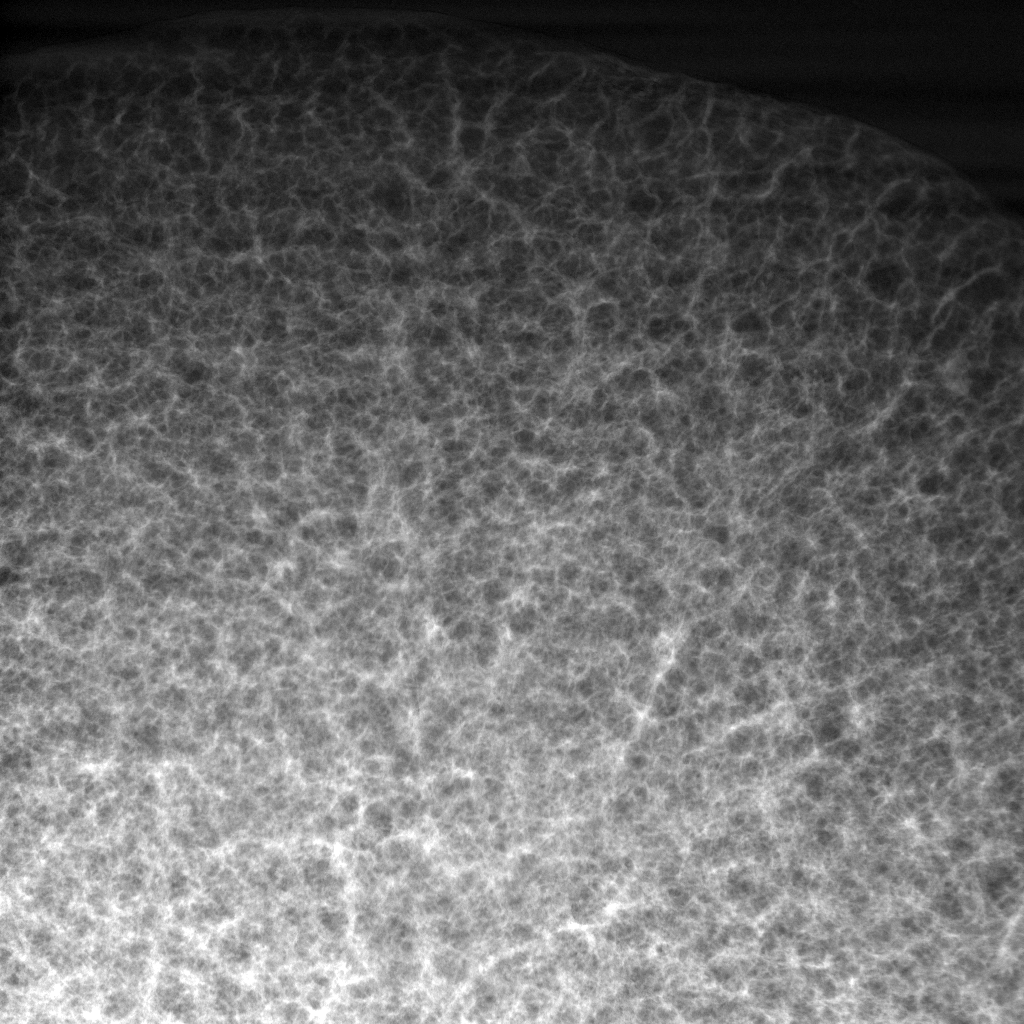
\includegraphics[width=\imagewidth]{img/tif-sin-rec/L-XXI-18_B50287-correctedprojection}};
				% 1024px = 1.5155mm > 100px = 148um > 338px = 500um, 68px = 100um
				%\draw[|-|,thick] (0,512) -- (1024,512) node [sloped,midway,above] {\SI{1.5155}{\milli\meter} (1024px)};
				\draw[white,|-|,thick] (\x,\y) -- (\x+338,\y) node [midway, above] {\SI{500}{\micro\meter}};
			\end{tikzpicture}%			
			\label{subfig:cpr}%
			}%
	}%
	\caption[Correction of the projections with flat images]{Correction of the raw recorded projections with the flat images. \subref{subfig:pi}: Recorded projection image. A set of these is the output of one tomographic scanning session. \subref{subfig:fi}: Flat image; obtained at the start of the scan to record the beam profile. \subref{subfig:cpr}: Corrected projection obtained after \autoref{eq:cpr} has been applied on the projection and flat image shown in panels \subref{subfig:pi} and \subref{subfig:fi}. All three images have a size of 1024$\times$1024 pixels with a size of \SI{1.48}{\micro\meter} each and are from a dataset of a rat lung.}
	\label{fig:corrected projection}%
	\todo[inline]{L-XXI-18, beamtime 2010a, Matthias Roth --> Add details in Caption}%
\end{figure}

The corrected projections are then transformed into so-called sinograms, where the $n$\textsuperscript{th} sinogram is composed of the $n$\textsuperscript{th} line of each projection. From one tomographic scan with 1500 projections recorded with a detector with a size of 2048$\times$2048 pixels, we get a set of 1024 sinograms with a size of 1024$\times$1500 pixels each.

Sinograms inherit their name because the Radon transformation\graffito{The Radon transformation was described in 1917 by Johann \citet{Radon1917} and is the mathematical basis for tomographic imaging.} of a Dirac delta peak resembles a sine wave. The Radon transformation of a cluster of objects appears as an overlay of blurred sine waves with different amplitudes and phases, as shown in \autoref{subfig:sin}, since any object can be considered as a collection of many small points.

One sinogram contains the total information of one plane or slice of the reconstructed tomographic image. We can thus reconstruct the $n$\textsuperscript{th} slice of the tomographic dataset from the $n$\textsuperscript{th} sinogram using different reconstructing algorithms, e.g.\ a standard filtered back-projection algorithm. In a reconstructed slice, the absorption properties of the sample at a certain height are encoded by the gray values of the image, as shown in \autoref{subfig:rec}. This virtual slice into a rat lung sample is part of a dataset permitting a fully three-dimensional, unrestricted view into the sample in a non-destructive way.

\renewcommand{\imsize}{0.705\linewidth}%sqrt(2)/2
\begin{figure}%
	\noindent\makebox[\textwidth]{%
		\subfloat[resized Sinogram]{%
			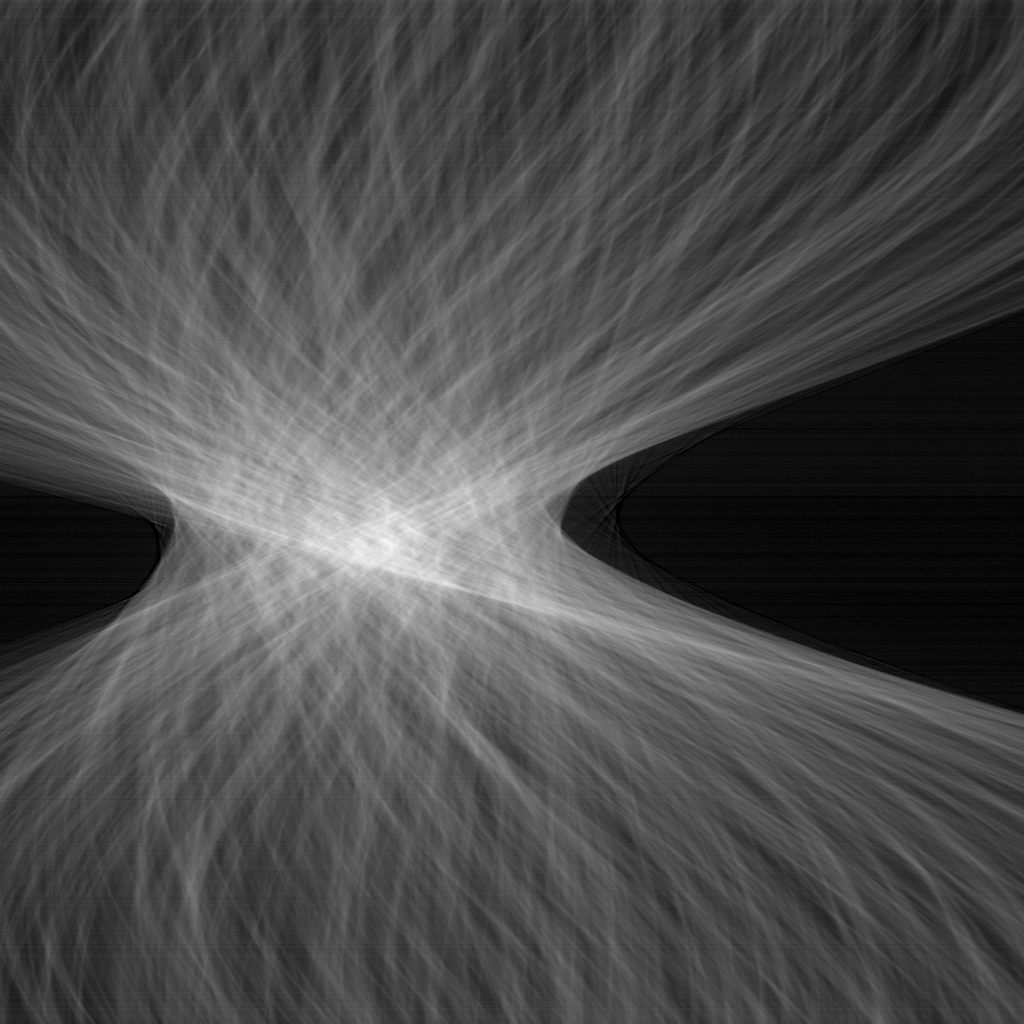
\includegraphics[width=\imsize]{img/tif-sin-rec/L-XXI-18_B50501-sin-DMP-scaled}%
			\label{subfig:sin}%
		}%
		\subfloat[Reconstructed Slice]{%
			\pgfmathsetlength{\imagewidth}{\imsize}%
			\pgfmathsetlength{\imagescale}{\imagewidth/1024}%
			\begin{tikzpicture}[x=\imagescale,y=-\imagescale]
				\def\x{633} % scalebar-x at golden ratio of x=1024px
				\def\y{922} % scalebar-y at 90% of height of y=1024px
				\node[anchor=north west, inner sep=0pt, outer sep=0pt] at (0,0) {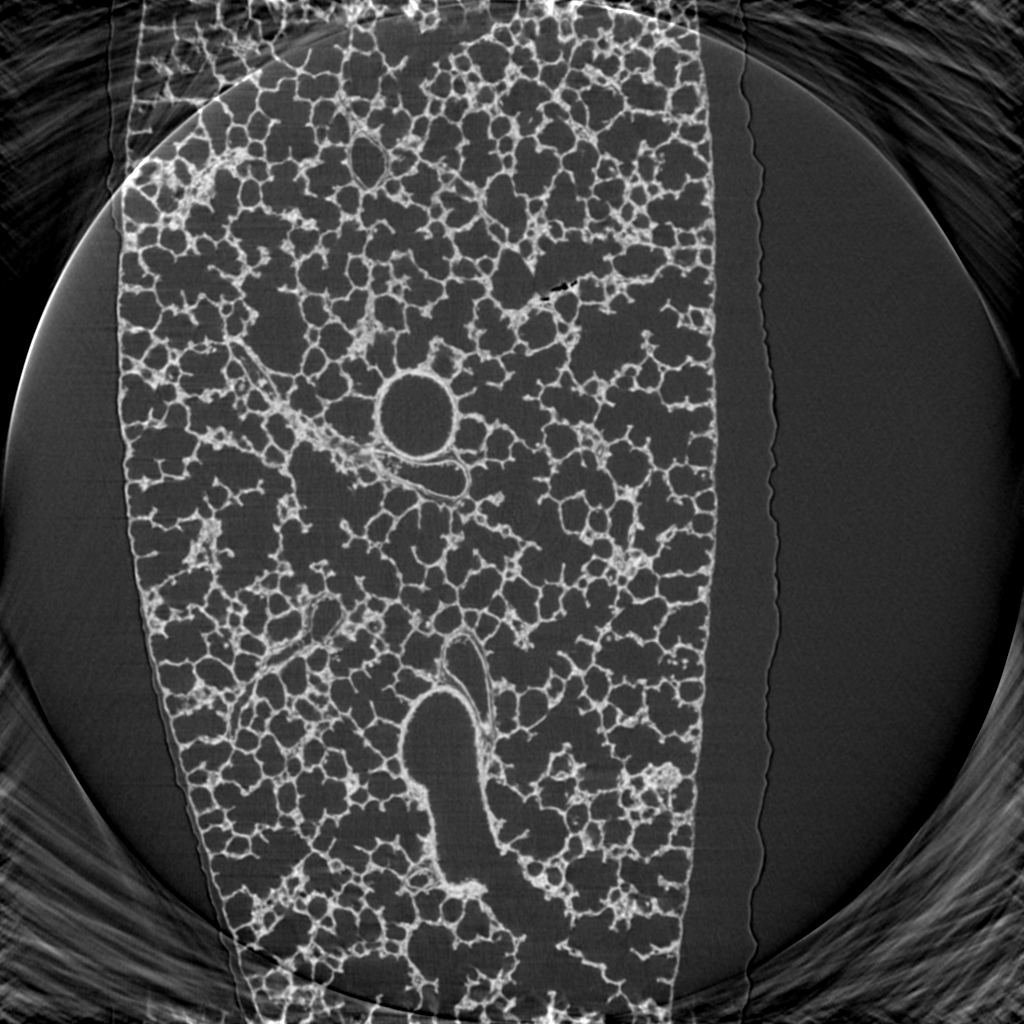
\includegraphics[width=\imagewidth]{img/tif-sin-rec/L-XXI-18_B50761-rec-8bit}};
				% 1024px = 1.5155mm > 100px = 148um > 338px = 500um, 68px = 100um
				%\draw[white,|-|,thick] (0,512) -- (1024,512) node [sloped,midway,above] {\SI{1.5155}{\milli\meter} (1024px)};
				\draw[white,|-|,thick] (\x,\y) -- (\x+338,\y) node [midway, above] {\SI{500}{\micro\meter}};
			\end{tikzpicture}%
			\label{subfig:rec}%
		}%
	}%
	\caption[Sinogram and Reconstruction]{Sinogram and Reconstruction of the projections of the rat lung sample shown in \autoref{fig:corrected projection}. \subref{subfig:sin}: The $n$\textsuperscript{th} sinogram has been obtained after reordering the $n$\textsuperscript{th} line of each of the 1501 corrected projections. The sinogram has been rescaled to a square format for display purposes, it would have a size of 1024$\times$1501 pixels. It doesn't really make sense to draw a scalebar on a sinogram, it has thus been omitted. \subref{subfig:rec}: The tomographic reconstruction of the complete set of sinograms results in a set of 1024 reconstructed slices with 1024$\times$1024 pixels of a size of \SI{1.48}{\micro\meter} each. A set of such slices is then used for further processing, measuring and three-dimensional visualization.}
	\label{fig:Sin Rec}
		\todo[inline]{L-XXI-18, beamtime 2010a, Matthias Roth --> Add details in Caption}%
\end{figure}

The amount of scanned projections---the number of angles at which projections have been recorded---is defined by the so-called sampling theorem. The sampling theorem as defined by \citet{Shannon1949} states that: \begin{quote}If a function $f(t)$ contains no frequencies higher than $W$ cps, it is completely determined by giving its ordinates at a series of points spaced $1/2\ W$ seconds apart. \cite{Shannon1949}\end{quote}

Paraphrased to tomographic imaging, the sampling theorem states that the minimal number of recorded angles along the rotation of the sample must be at least equal to twice the highest frequency used to scan the sample.

From calculations in polar coordinates one can deduce that for a detector with the size $N$ $M=\frac{\pi}{n}N$ angular projections are required to fulfill the sampling theorem for tomographic reconstruction~\cite{Stampanoni2002a}. Generally, for well-balanced reconstructed image with a size of $N\times N$ pixels, recorded with a detector of the same size, the total number of projections should be roughly equal to $N$~\cite{Kak2002}. In in layman's terms, we can thus say that if we scan a sample with a detector of 1024$\times$1024 pixels, we need to record approximately 1000 projections over a sample rotation of \SI{180}{\degree}.

At \ac{tomcat} this rule of thumb is exactly obeyed in the case of a tomographic scan with a binned\graffito{Binning is the process where 2$\times$2 pixels on the camera are averaged to one pixel, both to reduce the image size and noise.} detector. For a standard scan with an unbinned detector---resulting in images with a size of 2048$\times$2048 pixels---only 1500 projections are acquired, thus violating the rule. But even with this seemingly undersampled data acquisition, reconstructions with very high quality are obtained.

\autoref{ch:haberthuer2010} presents a scanning method where the sampling theorem is deliberately violated both to increase the field of view of \ac{tomcat} and to reduce the radiation dose imparted on the sample.

For classic tomographic imaging, an x-ray tube is used as a source of radiation. In \ac{srxtm}, which was used to obtain the tomographic data for this thesis---as the name suggests---x-rays from a synchrotron are used as a radiation source. The following sections give a short overview over the underlying theory of the synchrotron radiation and a quick rundown on the \ac{sls} and the beamline where all the presented experiments have been carried out.

\section{Synchrotron Radiation}
Synchrotron facilities use the fact that accelerated particles traveling on a curved trajectory emit radiation. If charged particles at relativistic speed undergo a change of direction (\ie in a magnetic field) so-called synchrotron radiation is emitted. 

Synchrotron radiation was first observed as energy loss in electron storage rings used for high energy physics experiments. First generation synchrotron sources for scientific use were beamports at such storage ring facilities, which utilized otherwise lost radiation. Dedicated second-generation synchrotron radiation sources have been built over the years; these were ring-like structures using a series of magnets to control the accelerated particles. Current---third-generation---synchrotron radiation facilities are composed of many straight sections of different lengths, specially optimized to accommodate different magnetic structures used to generate the synchrotron radiation~\cite{Stampanoni2002a,Margaritondo2002,wwwsls}. 

\subsection{Bending Magnets, Undulators and Wigglers}
The three magnetic structures used in synchrotron facilities are bending magnets, undulators and wigglers. All three emit radiation with different characteristics and intensities.

Bending magnets\graffito{Such magnets are also used in traditional televisions, which contain a cathode ray tube, which is essentially a small particle accelerator. They move the electron beam over the screen of the TV tube in a controlled fashion.~\cite{wiki:dipolemagnet}} are used to create a homogeneous magnetic field over a defined distance. The magnetic field inside forces accelerated particles injected into the bending magnet to travel on a circular trajectory. The result is a fan of radiation in the tangential direction of the bend.

\begin{figure}
	\noindent\makebox[\textwidth]{%
		\centering%
		\subfloat[]{%
			% !TEX root = ../Thesis.tex
%
%\documentclass{article}
%\usepackage{graphicx,tikz}
%\usepackage[graphics,tightpage,active]{preview}
%\PreviewEnvironment{tikzpicture}
%\begin{document}
%%%%%%%%%%%%%%%%%%%%%%%%%%%%%%%%%%%%%%%%%%%%%%%%%
	\begin{tikzpicture}
		%\draw [help lines] (0,0) grid (5,5);
		% electron arc
			\draw [<-] (0,0) arc (90:110:10) node [above] {$e^-$} arc (110:120:10);
			\draw [->] (0,0) arc (90:60:10);
		% beam angle
			\draw (5,0) arc (0:-25:2);
			\draw (5,0) arc (0:25:2) node [right] {$\frac{1}{\gamma}$};
		% beam
			\def\alpha{4}
			\def\length{6}
			\def\arclength{0.41956087166106248200152636193909} % arclength = tan(\alpha)*\length
			\fill [color=red,nearly opaque] (0,0) -- (\alpha:\length) arc (90+\alpha:-90-\alpha:\arclength) -- cycle; 
			\draw (\alpha:\length) arc (90+\alpha:-90-\alpha:\arclength);
			\node at (3,.5) {$\lambda$};
		% arrows
			\draw [->] (0,0) -- (\alpha:\length);
			\draw [->] (0,0) -- (\length+\arclength,0);
			\draw [->] (0,0) -- (-\alpha:\length);
	\end{tikzpicture}
%%%%%%%%%%%%%%%%%%%%%%%%%%%%%%%%%%%%%%%%%%%%%%%%%
%\end{document}%
			\label{subfig:bend}%
			}%
		\hspace{4mm}%
		\def\width{.309\linewidth}%
		\def\height{.309\linewidth}%
		\subfloat[]{%
			%\documentclass{article}
%\usepackage{tikz,pgfplots,siunitx}
%\usepackage[graphics,tightpage,active]{preview}
%\PreviewEnvironment{tikzpicture}
%\begin{document}
%%%%%%%%%%%%%%%%%%%%%%%%%%%%%%%%%%%%%%%%%%%%%%%%%%%%%%%%%%%%%%
%\pgfplotsset{xlabel=$\hbar \omega$,ylabel=F}
\begin{tikzpicture}
	\begin{axis}[%
		width=\width,%
		height=\height,%
		scale only axis,%
		axis x line=bottom,%
		axis y line=left,%
		ticks=none,%
		xmin=0,%
		xmax=1.5,%
		ymin=0,%
		ymax=1,%
		%mark=triangle
		]
		\addplot [fill=lightgray,thick]
			coordinates 
				{
					(0,0)
					(0.0001,0.12)
					(0.596441,0.52003)
					(0.6178	,0.532352)
					(0.645266,0.547748)
					(0.675886,0.553743)
					(0.703409,0.562888)
					(0.734057,0.565758)
					(0.764735,0.565502)
					(0.795441,0.562121)
					(0.823136,0.552516)
					(0.847822,0.536685)
					(0.872536,0.517729)
					(0.897279,0.495648)
					(0.915916,0.470492)
					(0.934552,0.445337)
					(0.950121,0.420207)
					(0.965689,0.395078)
					(0.975151,0.366874)
					(0.990749,0.338619)
					(1.00021,0.310415)
					(1.01274,0.282185)
					(1.02223,0.250856)
					(1.10429,0)
					(1.5,0)
				};
	\end{axis}
\end{tikzpicture}%
%%%%%%%%%%%%%%%%%%%%%%%%%%%%%%%%%%%%%%%%%%%%%%%%%%%%%%%%%%%%%%
%\end{document}%
			\label{subfig:bend-spectrum}%
			}%
		}
	\caption[Bending magnet radiation]{Bending magnet radiation of wavelength $\lambda$ produced by a relativistic electron traveling in an uniform magnetic field. %
		\subref{subfig:bend}: Electrons execute a circular motion with acceleration directed towards the center. The radiation is directed tangentially outward in a narrow radiation cone with an emission angle of typically $\frac{1}{\gamma}$ where $\gamma$ is the Lorentz contraction factor. %
		\subref{subfig:bend-spectrum}: The radiation spectrum is very broad, analogous to a ``white light'' x-ray light bulb.%
		Adapted from~\cite{Attwood2007}.}% http://is.gd/biHF4
	\label{fig:bending magnets}
\end{figure}

\begin{figure}
	\noindent\makebox[\textwidth]{%
		\centering%
		\subfloat[]{%
			% !TEX root = ../Thesis.tex
%
%\documentclass{article}
%\usepackage{graphicx,tikz}
%\usepackage[graphics,tightpage,active]{preview}
%\PreviewEnvironment{tikzpicture}
%\begin{document}
%%%%%%%%%%%%%%%%%%%%%%%%%%%%%%%%%%%%%%%%%%%%%%%%%
	\begin{tikzpicture}
		%\draw [help lines] (0,0) grid (5,5);
		\def\a{120}	% 90+40
		\def\b{60}		% 90-40 
		\def\c{-120}
		\def\d{-60}
		\def\length{0.5}
		\def\start{-.5}
		% travelling electron
			\node [anchor=east] at (\start,0) {$e^{-}$};
			\draw [->] (\start,0) arc (\a:\b:\length) arc (\c:\d:\length) arc (\a:\b:\length) arc (\c:\d:\length) arc (\a:\b:\length) arc (\c:-90:\length);
		% beam angle
		\clip (2.5,-1.25) rectangle (6.125,1.25);
			\draw (5,0) arc (0:-25:2);
			\draw (5,0) arc (0:25:2) node [right] {$\frac{1}{\gamma\sqrt{N}}$};
		% beam
			\def\alpha{1}
			\def\length{6}
			\def\arclength{0.10473038956930551459077337131837} % arclength = tan(\alpha)*\length
			\fill [color=red,nearly opaque] (0,0) -- (\alpha:\length) arc (90+\alpha:-90-\alpha:\arclength) -- cycle; 
			\draw (\alpha:\length) arc (90+\alpha:-90-\alpha:\arclength);
			\node at (3.5,.25) {$\lambda$};
		% arrows
			\draw (0,0) -- (\alpha:\length);
			\draw [->] (0,0) -- (\length+\arclength,0);
			\draw (0,0) -- (-\alpha:\length);
	\end{tikzpicture}
%%%%%%%%%%%%%%%%%%%%%%%%%%%%%%%%%%%%%%%%%%%%%%%%%
%\end{document}%
			\label{subfig:undulator}%
			}%
		\hspace{4mm}%
		\def\width{.309\linewidth}%
		\def\height{.309\linewidth}%
		\subfloat[]{%
			% !TEX root = ../Thesis.tex
%\documentclass{article}
%\usepackage{tikz,pgfplots,siunitx}
%\usepackage[graphics,tightpage,active]{preview}
%\PreviewEnvironment{tikzpicture}
%\def\width{\linewidth}
%\def\height{\linewidth}
%\begin{document}
%%%%%%%%%%%%%%%%%%%%%%%%%%%%%%%%%%%%%%%%%%%%%%%%%%%%%%%%%%%%%%
%\pgfplotsset{xlabel=$\hbar \omega$,ylabel=F}
\begin{tikzpicture}
	\begin{axis}[%
		width=\width,%
		height=\height,%
		scale only axis,%
		axis x line=bottom,%
		axis y line=left,%
		ticks=none,%
		xmin=0,%
		xmax=1.5,%
		ymin=0,%
		ymax=1,%
		%mark=triangle
		]
		%% or use code on http://is.gd/bk66S to make a nicer plot...
		\addplot [fill=lightgray,thick]
			coordinates 
				{
	  				(0,0)
					(0.30,0.00425626)
					(0.333874,0.00950491)
					(0.339687,0.0335484)
					(0.341953,0.0870162)
					(0.352407,0.62)
					(0.385544,0.0681442)
					(0.389051,0.0413938)
					(0.392557,0.0146433)
					(0.448396,0)
					(0.695832,0.00286691)
					(0.707956,0.0188665)
					(0.716904,0.0402249)
					(0.726472,0.02147439)
					(0.73604,0)
					(1.04534,0.00162091)
					(1.05746,0.0176205)
					(1.05973,0.0710883)
					(1.06014,0.0443489)
					(1.0624	,0.0978167)
					(1.07164,0.100458)
					(1.07515,0.0737071)
					(1.07861,0.0496306)
					(1.08212,0.0228801)
					(1.08864,0)
					(1.5,0)
				};
	\end{axis}
\end{tikzpicture}%
%%%%%%%%%%%%%%%%%%%%%%%%%%%%%%%%%%%%%%%%%%%%%%%%%%%%%%%%%%%%%%
%\end{document}%
			\label{subfig:undulator-spectrum}%
			}%
		}
	\caption[Undulator radiation]{Undulator radiation is generated as a highly relativistic electron traverses a periodic magnetic field.%
		\subref{subfig:undulator}: The magnetic field in an undulator is relatively weak and the resultant angular excursions of the electron are smaller than the angular width of the natural radiation cone, $\frac{1}{\gamma}$, normally associated with synchrotron radiation.%
		\subref{subfig:undulator-spectrum}: The frequency spread of undulator radiation can be very narrow, and the radiation can be extremely bright and partially coherent, under certain circumstances. The characteristic emission angle is narrowed by a factor $\sqrt N$, where $N$ is the number of magnetic periods. Typically $N$ is of order 100. Depending on the magnet strength, harmonic radiation may be generated. Adapted from~\cite{Attwood2007}.}%http://is.gd/biHF4
	\label{fig:undulator}
\end{figure}

\begin{figure}
	\noindent\makebox[\textwidth]{%
		\centering
		\subfloat[]{%
			% !TEX root = ../Thesis.tex
%
%\documentclass{article}
%\usepackage{graphicx,tikz}
%\usepackage[graphics,tightpage,active]{preview}
%\PreviewEnvironment{tikzpicture}
%\begin{document}
%%%%%%%%%%%%%%%%%%%%%%%%%%%%%%%%%%%%%%%%%%%%%%%%%
	\begin{tikzpicture}
		%\draw [help lines] (0,0) grid (5,5);
		\def\a{130}	% 90+60
		\def\b{50}		% 90-40 
		\def\c{-130}
		\def\d{-50}
		\def\length{0.75}
		\def\start{-1.2}
		% travelling electron
			\node [anchor=east] at (\start,0) {$e^{-}$};
			\draw [->] (\start,0) arc (\a:\b:\length) arc (\c:\d:\length) arc (\a:\b:\length) arc (\c:-90:\length);
		% beam angle
		\clip (2.5,-1.5) rectangle (7,1.75);
			\draw (5,0) arc (0:-25:3);
			\draw (5,0) arc (0:25:3) node [right] {$\gg\frac{1}{\gamma}$};
		% beam
			\def\alpha{6}
			\def\length{6}
			\def\arclength{0.63062541159405877506901428083929} % arclength = tan(\alpha)*\length
			\fill [color=red,nearly opaque] (0,0) -- (\alpha:\length) arc (90+\alpha:-90-\alpha:\arclength) -- cycle; 
			\draw (\alpha:\length) arc (90+\alpha:-90-\alpha:\arclength);
			\node at (3.5,.75) {$\lambda$};
		% arrows
			\draw [->] (0,0) -- (\alpha:\length);
			\draw [->] (0,0) -- (\length+\arclength,0);
			\draw [->] (0,0) -- (-\alpha:\length);
	\end{tikzpicture}
%%%%%%%%%%%%%%%%%%%%%%%%%%%%%%%%%%%%%%%%%%%%%%%%%
%\end{document}%
			\label{subfig:wiggler}%
			}%
		\hspace{4mm}%
		\def\width{.309\linewidth}%
		\def\height{.309\linewidth}%
		\subfloat[]{%
			\documentclass{article}
\usepackage{tikz,pgfplots,siunitx}
\usepackage[graphics,tightpage,active]{preview}
\PreviewEnvironment{tikzpicture}
\begin{document}
%%%%%%%%%%%%%%%%%%%%%%%%%%%%%%%%%%%%%%%%%%%%%%%%%%%%%%%%%%%%%%
\pgfplotstableread{plotdata/graph_wiggler.txt}\table
%\pgfplotstableread{Plots/plotdata/InteractionPercentage-big.txt}\table
%\pgfplotsset{
%	legend style={
% 		%at={(1.02,0.5)}, anchor=west,%left
% 		at={(0.5,-0.2)}, anchor=north,%bottom
%		cells={anchor=west},
%		%font=\footnotesize,
%		},
%	xlabel=Photon Energy [\kilo\electronvolt],%
%	ylabel=[\percent]
%	}
\begin{tikzpicture}
	\begin{axis}[%
		%width=\width,%
		%height=\height,%
%		scale only axis,%
		axis x line=bottom,%
		axis y line=left,%
		ticks=none,%
%		grid=none%
%		no markers,
		xmin=0,%
		%xmax=1e5,%
		ymin=0,%
		%ymax=100,%
		]
		\addplot [fill=lightgray,thick]
			table [x=x, y=Curve1] from \table;
		%\legend{Curve1	}
	\end{axis}
\end{tikzpicture}%
%%%%%%%%%%%%%%%%%%%%%%%%%%%%%%%%%%%%%%%%%%%%%%%%%%%%%%%%%%%%%%
\end{document}%
			\label{subfig:wiggler-spectrum}%
			}%
		}
	\caption[Wiggler radiation]{Wiggler radiation is also generated from a periodic magnet structure. %
		\subref{subfig:wiggler}: In the strong magnetic field the angular excursions are significantly greater than the natural ($\frac{1}{\gamma}$) radiation cone. Because accelerations are stronger in this limit, the radiation generated peaks at higher photon energies and has both a higher photon flux and more power. %
		\subref{subfig:wiggler-spectrum}: The radiation spectrum is very broad, similar to that of the bending magnet. Although more power is radiated, wiggler radiation is less bright because of the substantially increased radiation cone. Adapted from~\cite{Attwood2007}.}% http://is.gd/biHF4
	\label{fig:wiggler}
\end{figure}

Undulators consist of periodic structures of dipole magnets with relatively weak fields. The alternating static magnetic field forces the electrons to harmonically oscillate as they move in the axial direction, resulting in an undulating motion of the particles inside the structure. The weak magnetic fields cause small amplitude undulation which leads to a narrow radiation cone as a result. Through coherent addition of the tightly confined electron beam, the produced radiation is emitted with small angular divergence and concentrated in narrow energy bands~\cite{Stampanoni2002a}.

Wigglers are the strong brothers of the undulators. Due to stronger magnetic fields the oscillation amplitude of the electrons and the emitted radiation power are larger and the radiation cone is broader.

The relativistic electrons inside the storage ring are usually produced by a hot filament and subsequently pre-accelerated and injected into the storage ring by a linear accelerator. Bending magnets along the storage ring keep the electrons on their circular path. Quadrupole magnets along the ring are used to improve the geometrical characteristics of the electron beam, \ie reduce the transverse section and angular spread of the beam, hence improving the so-called brightness of the source~\cite{Margaritondo2002}.

Using one of the three above mentioned structures, the radiation is then outcoupled of the storage ring and transferred into the measuring hut. At \ac{tomcat} the radiation is outcoupled using a very strong bending magnet, a so-called superbend, which is described in detail below.

\section{The Swiss Light Source}
The \ac{sls} at the \ac{psi} in Villigen, Switzerland is a third-generation synchrotron light source. With an energy of \SI{2.4}{\giga\electronvolt}, it provides photon beams of high brightness for research in materials science, biology and chemistry.

\renewcommand{\imsize}{0.618\linewidth}%
\begin{figure}
	\centering
	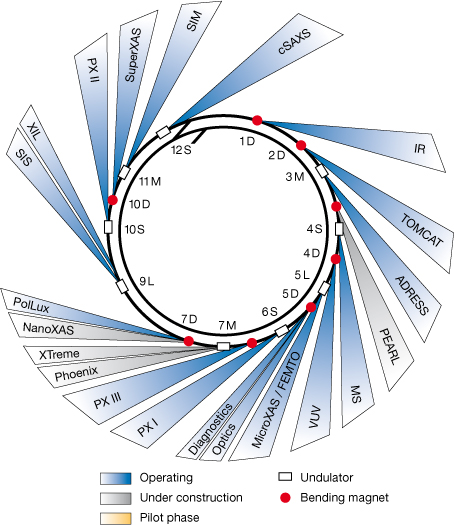
\includegraphics[width=\imsize]{img/SLS_beamlines_2008}
	\caption[Beamlines at the Swiss Light Source]{Beamlines at the \ac{sls}. Image from the \href{http://sls.web.psi.ch/view.php/beamlines/}{SLS Website}}
	\label{fig:beamlines}
	\todo[inline]{I've asked Marco for higher resolution image\ldots}%
\end{figure}

\section{TOMCAT}\label{sec:tomcat}
At the beamline for \acf{tomcat} the user can perform absorption as well as phase contrast imaging with an isotropic voxel\graffito{A voxel or volumetric pixel is the \threed analogy to a \twod pixel.} size ranging from \SI{350}{\nano\meter} up to \SI{14.8}{\micro\meter}, depending on the chosen magnification. Typical acquisition times are in the order of a few minutes for a full sample, depending on the selected energy and resolution.

\citet{Stampanoni2006a} described the \ac{tomcat} beamline in detail, a short rundown on the most important features are presented here: The beamline is located at the X02DA port of the SLS and started regular user operation in June 2006. Synchrotron light is delivered by a \SI{2.9}{\tesla} bending magnet with a magnetic field more than double the strength of the normal \ac{sls} bending magnets. This enables to have a high critical energy of the source (\SI{11.1}{\kilo\electronvolt}, corresponding to a wavelength of \SI{1.22}{\angstrom}) and results in a considerable increase of flux\graffito{Flux is defined as the amount of particles, mass or energy which flows through an area in a certain time and essentially describes the brightness of the beam} at the desired energy range.

Because of the high coherence of the used synchrotron radiation is desired to be kept until the radiation penetrates the sample, a minimization of the optical elements was targeted during the design of the beamline. A \SI{100}{\micro\meter} thick diamond window separates the ultra high vacuum (\SI{e-10}{\millibar}) from the vacuum section of the beamline (\SI{e-7}{\millibar}). After the beam passes the diamond window, its energy is selected using a double crystal multilayer monochromator (Strumenti Scientifici CINEL s.r.l., Padova, Italy). This main optical component of the beamline covers an energy range of 6--\SI{45}{\kilo\electronvolt} with a bandwidth of a few percent down to a few permille~\cite{Stampanoni2006a}.

After collimation, the beam travels through an evacuated pipe into the measuring hut and is directed towards the sample. The sample sits atop a high precision sample manipulator (resolution better than \SI{1}{\micro\meter}, the manipulator is shown in \autoref{fig:tomcat}) which is used for centering the sample in the beam and for the rotation of the sample for tomographic imaging. 

The x-rays which penetrated the sample are detected using a combination of a scintillator, microscope optics and a \ac{ccd}-camera. The scintillator\graffito{The latin word \textit{scintillare} can be translated with sparkling or flickering.} converts incident x-rays to visible light through fluorescence. Charged particles excite the scintillator material and this excitation energy is then subsequently emitted by fluorescence photons at a longer wavelength, which makes it possible to detect the incident beam using a \ac{ccd}-camera. The camera at \ac{tomcat} features a detector with 2048$\times$2048 pixels with a size of 7.4$\times$\SI{7.4}{\micro\meter} each and can read out a full frame \SI{14}{\bit} image in \SI{260}{\millisecond}. Between the scintillator and the \ac{ccd}-sensor interchangeable microscope objectives enable to easily vary the pixel size range of the resulting tomographic reconstructions from 350$\times$\SI{350}{\nano\meter} up to 5.6$\times$\SI{5.6}{\micro\meter}. Depending on the chosen pixel size, the resulting field of view of a standard scan varies between 0.75$\times$\SI{0.75}{\milli\meter\squared} and 11.45$\times$\SI{11.45}{\milli\meter\squared}\graffito{See \autoref{ch:haberthuer2010} for a method to increase the field of view of tomography endstations while keeping the small voxel size.}.

\renewcommand{\imsize}{1.41\linewidth}%
\begin{figure}
	\noindent\makebox[\textwidth]{%
		\subfloat[Panoramic view]{%
			\includegraphics[width=\imsize]{img/TOMCAT_DSC_6725-DSC_6760_fused}%
			\label{subfig:TOMCATpano}%
		}%
	}%
	\\%
	\renewcommand{\imsize}{0.705\linewidth}%
	\noindent\makebox[\textwidth]{%
		\subfloat[Overview]{%
			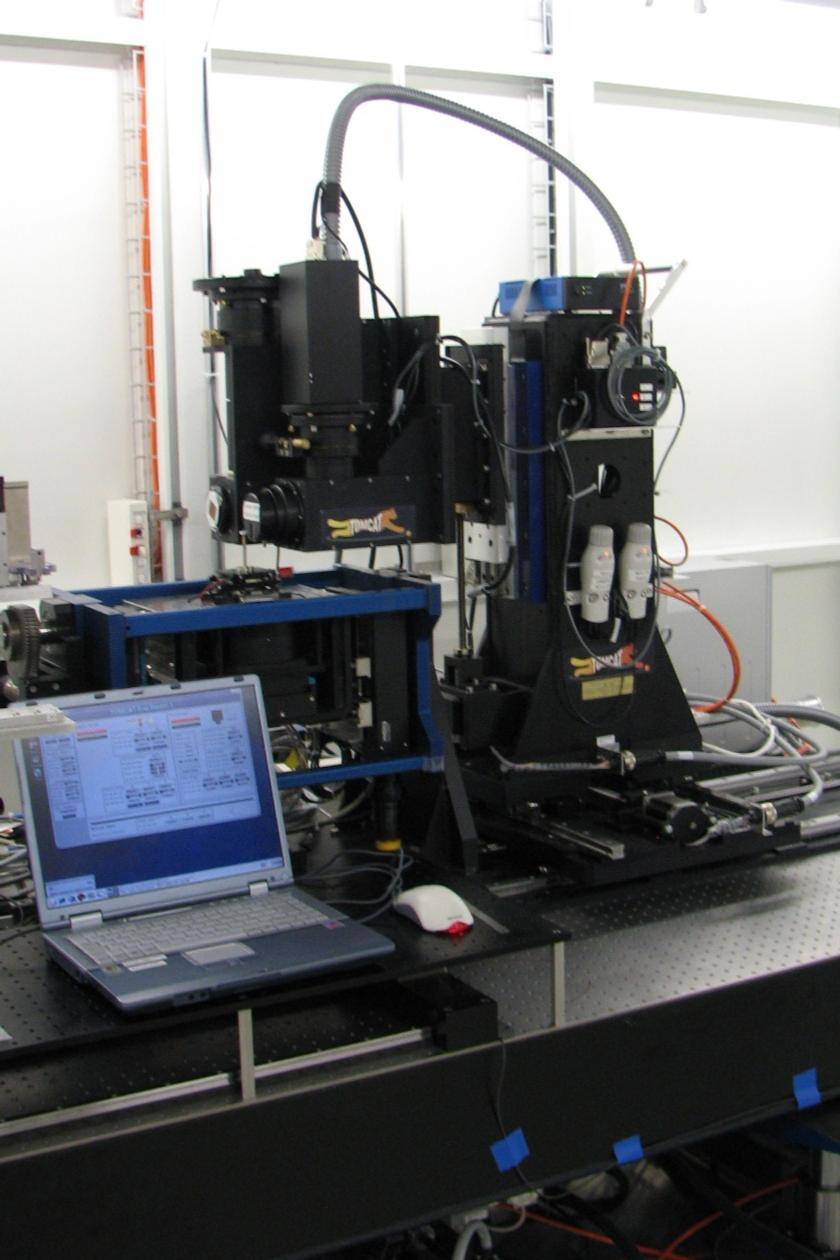
\includegraphics[width=\imsize]{img/TOMCAT1}%
			\label{subfig:TOMCAT1}%
		}%
		\subfloat[Detail]{%
			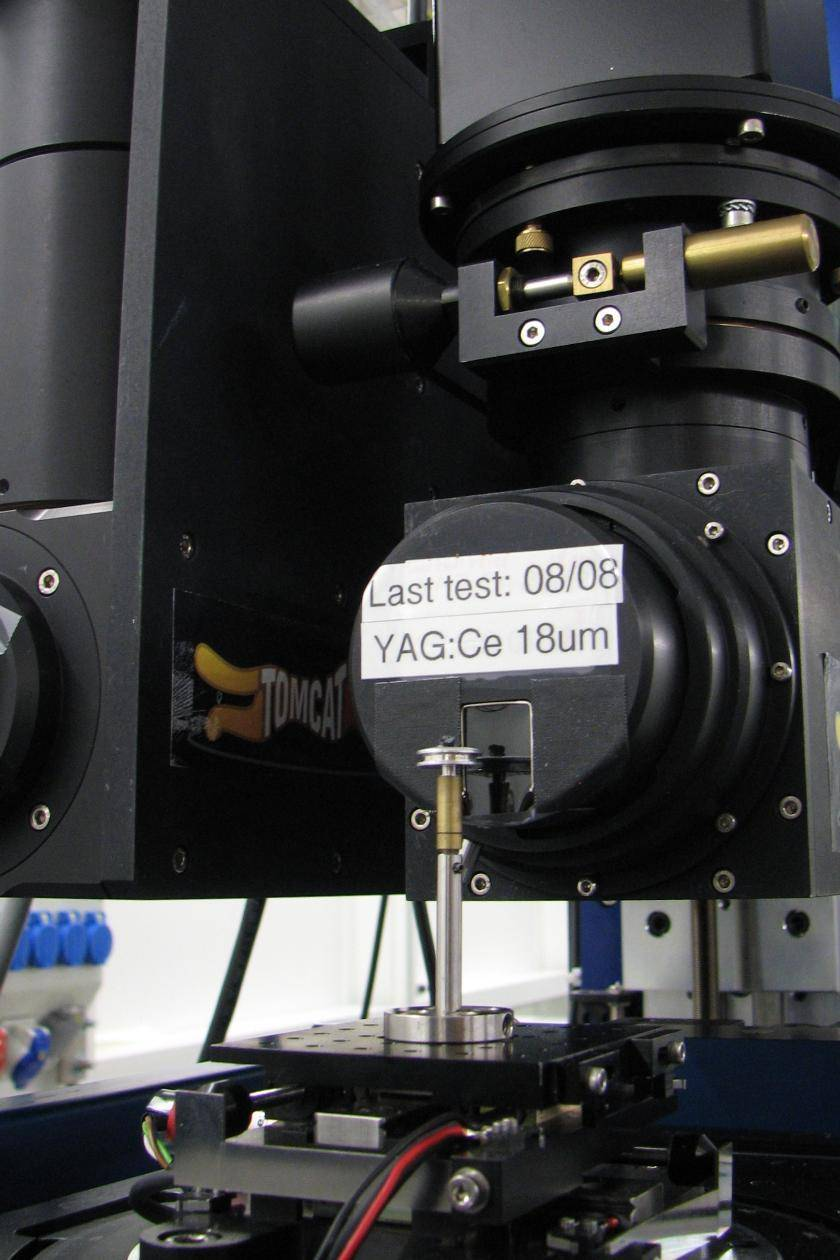
\includegraphics[width=\imsize]{img/TOMCAT2}%
			\label{subfig:TOMCAT2}%
		}%
	}%
	\caption[The \acs{tomcat} end station]{The \ac{tomcat} end station. \subref{subfig:TOMCATpano}: \SI{180}{\degree} panoramic view of the endstation. \subref{subfig:TOMCAT1}: Overview: The blue structure behind the control notebook is the sample stage with the sample holder on the rotation stage on top of it. The black structure above contains the scintillator, the microscope optics and the camera. \subref{subfig:TOMCAT2}: Detail of the microscope optics: The sample holder with a mounted standard electron microscopy sample table is carrying a small piece of a rat lung which can be seen in the reflection. The round structure behind the sample contains the different objectives. The reflecting rectangle visible under the label on the objective revolver is the scintillator which is used to convert the x-ray beam into visible light, which after magnification is then recorded with the \ac{ccd}-camera.}%
	\label{fig:tomcat}
\end{figure}

The sample positioning in the beam (using the sample stage shown in \autoref{fig:tomcat}) and the parameters of the scan---like exposure time, amount of projections, name, etc.---are controlled from outside the measuring hut through an \ac{epics}.

After the start has been started, sinograms are calculated on the fly and the tomographic reconstruction can be initialized using a web-based interface seconds after the scan has been finished. This interface and the general reconstruction workflow and management of the reconstruction cluster has been thoroughly described by \citet{Hintermueller2010}.

The web-based interface is used to submit the reconstruction of the tomographic datasets to a computing cluster of five \SI{64}{\bit} Opteron machines with four cores and \SI{8}{\giga\byte} \acs{ram} each. Immediately after reconstruction on the cluster the resulting data is copied to an external disk which makes it possible that the recorded tomographic datasets can be taken to the home laboratory immediately after the beamtime shifts.

This is where the real work starts\ldots
%%%%%%%%%%%%%%%%%%%%%%%
\cleardoublepage\myPart{Results}\label{part:results}
% !TEX root = ../Thesis.tex
\acresetall
\pdfbookmark[1]{Publications}{publications}
\myChapter{Publications}\label{ch:publications}
\begin{flushright}{\slshape I'm throwing rocks tonight. Mark it, Dude.} \\ \medskip
	--- Steve Buscemi\\as Donny in\defcitealias{TheBigLebowski}{The Big Lebowski}\citetalias{TheBigLebowski} \citep{TheBigLebowski}
\end{flushright}
\vspace{6cm}

The three chapters~\ref{ch:xrm2008}, \ref{ch:tsuda2008} and \ref{ch:haberthuer2010} of this document are copies of publications I have authored or collaborated on. They represent the published results achieved during the time frame of this thesis.

\section{\autoref{ch:xrm2008}}
\autoref{ch:xrm2008} contains a proceeding that has been published in the Conference Series of the \href{http://iopscience.iop.org/1742-6596/}{Journal of Physics} after the 9\textsuperscript{th} \href{http://xrm2008.web.psi.ch/}{International Conference on X-Ray Microscopy} in Zürich, Switzerland. The manuscript presents a method for localization and three-dimensional imaging of sub-micron gold particles in rat lungs. Two batches of gold particles with sizes of \SI{200}{\nano\meter} and \SI{700}{\nano\meter} have been applied to rat lung samples through intratracheal instillation. The samples have been scanned with high resolution \ac{srxtm} at the \ac{tomcat} beamline of the \ac{sls} with a voxel size of \SI{350}{\nano\meter}. This resolution was sufficient to detect the exact three-dimensional localization of single and clustered gold particles with a size of \SI{700}{\nano\meter} in alveoli, alveolar ducts and terminal bronchioli in the rat lung samples. 

As the particles with a diameter of \SI{200}{\nano\meter} were below the detection limit of \ac{tomcat}, we were only able to accurately localize them by \ac{tem}. For this, the samples was sectioned into \SI{300}{\nano\meter} thick sections and analyzed using \ac{tem}. We were able to verify the exact locations of the gold particles of both sizes in the lung tissue. Gold particles with a size of \SI{700}{\nano\meter} were localized in consecutive sections even if they were not directly visible on certain slices. Since these particles were pulled out of the resin, we sometimes only observed a hole were gold particles would have been expected.

The high correlation between the virtual sections of the tomographic dataset and the real sections imaged through \ac{tem} makes the combination of both imaging modalities very well suited to obtain the full unrestricted 3D access using \ac{srxtm} and to verify the localization of the particles in the 3D-space with very high resolution using \ac{tem}.

\section{\autoref{ch:tsuda2008}}
\autoref{ch:tsuda2008} presents a new image processing method for accurate three-dimensional reconstruction of the gas exchange region of the lung. The method has been published in the \href{http://jap.physiology.org/}{Journal of Applied Physiology} and is based on a \ac{fe} analysis of the tomographic datasets recorded at \ac{tomcat}. 

The datasets have been segmented using an iteratively determined threshold. This threshold was chosen to match computed morphological parameters of the resulting three-dimensional reconstruction with the stereologically\graffito{Stereology refers to the mathematical methods for defining these properties of an irregular three-dimensional structure using two-dimensional planar sections obtained by physical or optical imaging techniques~\cite{Hsia2010}.} determined real morphological parameters of samples from the same lungs.

In this work we have been able to highlight numerous advantages of a three-dimensional analysis of the reconstructions over traditional stereology. One of the most fundamental advantages of the tomographic analysis is the non-destructive method of obtaining the informations. Using traditional methods, the sample has to be cut into histological sections, which essentially destroys the integrity of the sample. Using the tomographic dataset, a thorough analysis of the inner structure of sample can also be carried out on slices, but these slices are virtual. Another advantage of the virtual slicing through the sample is that slices with arbitrary orientation can be generated throughout the sample as long as needed, and interesting regions can be iteratively improved.

\section{\autoref{ch:haberthuer2010}}
In \autoref{ch:haberthuer2010} I present the so-called \emph{wide field scanning} method developed in order to cover a larger field of view at \ac{tomcat}. This larger field of view was needed to enable the three-dimensional analysis of the functional lung unit, the so-called acinus which seems to be growing to a larger extent than previously described \cite{Massaro1985,Massaro1992}.

Additionally, since the smallest structures we need to unambiguously detect are the alveolar septa with a thickness of several micrometers, we need to obtain tomographic scans with large magnifications, \ie high resolution in the order of one micron. 

Generally, those two points can not be satisfied with a single tomographic scan, since an increase in the field of view can only be acquired with low magnification and vice-versa. The method presented in this chapter overcomes this limitation through merging of several high resolution scans to one scan overlapping a large field of view. Additionally---through optimization of the acquisition protocol---the scanning time is minimized, which greatly reduces the radiation dose inflicted on the sample, which is a first step towards in-vivo \ac{srxtm} at \ac{tomcat}.

This so-called \ac{wf-srxtm} was implemented as a proof of concept during my post-graduate master thesis of the \href{http://www.biomed.ee.ethz.ch/nds/}{Master of advanced Studies ETH in Medical Physics} in the \ac{tomcat} group. In the following months, the method has been refined into a scanning protocol and is now routinely applied to obtain tomographic datasets of rat lung samples with both large field of view and high resolution. This paper has been published in the \href{http://journals.iucr.org/s/}{Journal of Synchrotron Radiation}.
\bibliographystyle{unsrtnat}
\bibliography{../../references}
% !TEX root = ../Thesis.tex
\myChapter[Multimodal imaging of sub-micron particles]{Multimodal imaging for the detection of sub-micron particles in the gas-exchange region of the mammalian lung}\label{ch:xrm2008}

\newcommand{\footremember}[2]{\footnote{#2}\newcounter{#1}\setcounter{#1}{\value{footnote}}}%
\newcommand{\footrecall}[1]{\footnotemark[\value{#1}]} 

David Haberthür\footremember{ana}{Institute of Anatomy, University of Bern, Bern, Switzerland}\\
Manuela Semmler-Behnke\footremember{inhalation}{Institute for Inhalation Biology, Helmholtz Zentrum München, Germany}\\
Shinji Takenaka\footrecall{inhalation}\\
Wolfgang G. Kreyling\footrecall{inhalation}\\
Marco Stampanoni\footremember{psi}{Swiss Light Source, Paul Scherrer Institut, Switzerland}\textsuperscript{,}\footremember{eth}{Institute for Biomedical Engineering, University and ETH Zürich, Switzerland}\\
Akira Tsuda\footnote{Physiology Program, Harvard School of Public Health, US}\\
Johannes C. Schittny\footrecall{ana}\textsuperscript{,}\footnote{\href{mailto:schittny@ana.unibe.ch}{schittny@ana.unibe.ch}}\\\\
First published in: J. Phys.: Conf. Ser. 186 012040 (3pp)\\
\href{http://dx.doi.org/10.1088/1742-6596/186/1/012040}{doi:10.1088/1742-6596/186/1/012040}

\section{Abstract}
The deposition sites of inhaled aerosols in the gas-exchange region of the lung represent one of the key parameters needed for the understanding of the interaction between these particles and lung tissue. In order to develop a method for three-dimensional imaging of sub-micron particles in lung tissue we applied gold particles (200 and \SI{700}{\nano\meter}) to rat lungs by intratracheal instillation. The samples were scanned at the beamline for \acf{tomcat} at the \acl{sls}. The \SI{200}{\nano\meter} particles were slightly below the detection capabilities of \acs{tomcat}. Therefore, their localization was obtained only by electron microscopy. At a voxel size of \SI{350}{\nano\meter} we observed single and clustered gold particles (\SI{700}{\nano\meter}) in alveoli, alveolar ducts, and small bronchioli. The locations of the gold particles were verified by transmission electron microscopical serial sections. We observed a very high correlation between these two imaging modalities. We conclude that a combination of x-ray tomographic microscopy and electron microscopy allows the full unrestricted \threed localization of particles smaller than the resolution of x-ray tomographic microscopy. We are planning to use this method for the verification of the simulation of particle deposition in the airway tree.

\section{Objective}
To study the deposition of sub-micron particles in the mammalian lung, we used \ac{srxtm} to record tomographic images of lung samples with high resolution (\SI{350}{\nano\meter}). In addition to \ac{srxtm}, we used conventional \ac{tem} to obtain high resolution images (resolution smaller than \SI{1}{\nano\meter}).

\section{Materials and Methods}
We applied \SI{200}{\nano\meter} and \SI{700}{\nano\meter} gold particles to rat lungs by intratracheal instillation. Thirty minutes after instillation, the lungs were fixed with \SI{2.5}{\%} glutaraldehyde by vascular perfusion, stained according to standard protocols for \ac{tem} and embedded in Epon. The samples were shaped to cylinders with a diameter of either 0.6 or \SI{1.2}{\milli\meter} and a length of several millimeters using a watchmakers lathe and then scanned at \ac{tomcat}~\cite{Stampanoni2007}, the beamline for \acl{tomcat} at the \acl{sls} at the Paul Scherrer Institute in Villigen, Switzerland. The samples were scanned at a wavelength of \SI{11.5}{\kilo\electronvolt}, post processed on a 20-node Linux cluster using filtered backprojection, resulting in an image stack of 2048$\times$2048$\times$2048 pixels with isotropic voxels of \SI{350}{\nano\meter} side length. The samples were visualized in three dimensions using an isosurface computed with Imaris x64 5.72 (Bitplane AG, Switzerland) on an AMD 64-based windows computer~\cite{Tsuda2008}. After tomographic image acquisition serial sections of the sample were cut and processed for transmission electron microscopy~\cite{Mund2008}. 

\section{Results}
We have been able to observe single and clustered gold particles in alveoli, alveolar ducts, and small bronchioli while imaging them at a voxel side length of \SI{350}{\nano\meter} with the use of \ac{srxtm} (Fig.~\ref{subfig:imaris} and \ref{subfig:slice-srxtm}). We were able to verify the locations of the observed gold particles by \ac{tem} (Fig.~\ref{subfig:slice-em}). 

Particles with a size of \SI{200}{\nano\meter}---a size smaller than the resolution achievable at \ac{tomcat}---were imaged using \ac{tem} after selecting a particular alveolus in three dimensional visualizations obtained from \ac{srxtm} data. Thirty minutes after instillation, particles were observed in cells --- mainly macrophages --- as well as in airspace. Most of the particles located in the airspace were in close contact to protein precipitations (Data not shown).
\renewcommand{\imsize}{0.285\textwidth}
\begin{figure}[htb]
	\centering
	\subfloat[]{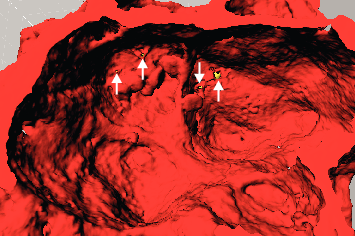
\includegraphics[height=\imsize]{img/XRM2008/imaris}\label{subfig:imaris}}\hfill
	\subfloat[]{\includegraphics[height=\imsize]{img/XRM2008/em/au900-1b-a}\label{subfig:slice-srxtm}}\hfill
	\subfloat[]{\includegraphics[height=\imsize]{img/XRM2008/em/au900-1b-b}\label{subfig:slice-em}}
	\caption[Three dimensional isosurface visualization of gold particles in the lung obtained from SRXTM data]{\subref{subfig:imaris}: Three dimensional isosurface visualization of gold particles in the lung obtained from \ac{srxtm} data. Gold grains (yellow) are deposited in terminal airspaces. The air-tissue interface was removed on top of the gold grains during the visualization process in order to show the gold particles (arrows). \subref{subfig:slice-srxtm}: Detailed view of virtual \ac{srxtm} section obtained at \ac{tomcat} containing two gold particles (arrows). The arrowheads are pointing to erythrocytes which are lighting up in the \ac{srxtm} images due to their high iron content of the hemoglobin. Due to the high contrast of gold the particles appear larger in the \ac{srxtm} images than they are in reality and we observed spiked image artifacts going out from the particles. \subref{subfig:slice-em}: Corresponding \ac{tem} section of the virtual \ac{srxtm} section. The thin black lines in \subref{subfig:slice-em} represent folds in the serial section. The white lines in \subref{subfig:slice-em} represent knife marks from the sectioning process.}
	\label{fig:imaris}
\end{figure}

\renewcommand{\imsize}{0.250\textwidth}
\begin{figure}[htb]
\centering
\subfloat[]{\includegraphics[width=\imsize]{img/XRM2008/em/au900-1b-c}\label{subfig:em-c}}\hfill
\subfloat[]{\includegraphics[width=\imsize]{img/XRM2008/em/au900-1b-d}\label{subfig:em-d}}\hfill
\subfloat[]{\includegraphics[width=\imsize]{img/XRM2008/em/au900-1b-e}\label{subfig:em-e}}\hfill
\subfloat[]{\includegraphics[width=\imsize]{img/XRM2008/em/au900-1b-f}\label{subfig:em-f}}\hfill
\caption[Transmission electron microscopy images of gold particles]{Transmission electron microscopy images of \SI{700}{\nano\meter} gold particles: \subref{subfig:em-c}--\subref{subfig:em-e}: Close-up view of square A of Fig.~\ref{subfig:slice-srxtm} showing a gold particle (arrows) in consecutive \ac{tem} sections which are \SI{80}{\nano\meter} apart. \subref{subfig:em-f}: Gold grain observed in square B in Fig.~\ref{subfig:slice-srxtm} (arrow). Roughly half of the gold grains observed were located inside the cells, \eg macrophages. The thin black lines visible in subfigures \subref{subfig:em-c}, \subref{subfig:em-e} and \subref{subfig:em-f} represent folds in the \ac{tem} section.}
\label{fig:srxtm-em}
\end{figure}

\section{Discussion}
A very high correlation between the two imaging modalities was observed. The virtual slices obtained from the \ac{srxtm} image stack (Fig.~\ref{subfig:slice-srxtm}) and the real slices obtained using \ac{tem} (Fig.~\ref{subfig:slice-em}) have only been corrected for rotation and magnification. The correct vertical position of the serial \ac{tem} section in the sample was obtained through rigorous alignment and precise positioning of the sample in the microtome.

We have been able to track the gold particles over consecutive serial sections, even if they sometimes were not directly visible. As can be seen in Fig.~\ref{subfig:em-e}, we sometimes only observed a hole where we would have expected to see the gold particle (arrow). Since the gold grains are much harder than Epon and do not stick well to the resin, it is expected that the grains will be pulled out of the Epon block as soon as half of the grain is cut.

\section{Conclusions}
We conclude that the combination of \ac{srxtm} and \ac{tem} allows the three dimensional localization of particles in the mammalian lung. In a synergistic way, we used \ac{srxtm} to obtain the full unrestricted \threed access and \ac{tem} to verify the localization of the particles in the \threed-space with very high resolution. 

We are planning to use this method for the detection and localization of inhaled particles and as a mean of providing data for airflow simulation in the mammalian lung.

\section{Acknowledgments}
We thank Christoph Hinterm\"uller and Federica Marone for expert help at \ac{tomcat} and Bettina De Breuyn as well as Christoph Lehmann for the preparation of the samples. This work has been supported by Swiss National Science Foundation grant 3100A0-109874 and by US National Heart, Lung, and Blood Institute grant HL-070542.
%\bibliographystyle{plainnat}
%\label{app:bibliography} 
%\bibliography{../Bibliography,../../references,../Tsuda2008references}
% !TEX root = ../Thesis.tex
\acresetall
\myChapter[Finite element \threed reconstruction of the pulmonary acinus]{Finite element \threed reconstruction of the pulmonary acinus imaged by synchrotron X-ray tomography}\label{ch:tsuda2008}

%\newcommand{\footremember}[2]{\footnote{#2}\newcounter{#1}\setcounter{#1}{\value{footnote}}}%
%\newcommand{\footrecall}[1]{\footnotemark[\value{#1}]} 

Akira Tsuda\footremember{boston}{School of Public Health, Harvard University, Boston, Massachusetts, USA}\textsuperscript{,}\footnote{Address for reprint requests and other correspondence: A. Tsuda, Molecular and Integrative Physiological Sciences, Harvard School of Public Health, 665 Huntington Ave., Boston, MA 02115 (e-mail: \href{mailto:atsuda@hsph.harvard.edu}{atsuda@hsph.harvard.edu}).}\\%
Nenad Filipovic\footnote{University of Kragujevac, Kragujevac, Serbia}\\%
David Haberthür\footremember{ana2}{Institute of Anatomy, University of Bern, Bern, Switzerland}\\%
Rene Dickie\footrecall{boston}\\%
Yasuto Matsui\footnote{Graduate School of Engineering, University of Kyoto, Kyoto, Japan}\\%
Marco Stampanoni\footnote{Swiss Light Source, Paul Scherrer Institut, Villigen, Switzerland}\\%
Johannes C. Schittny\footrecall{ana2}\\\\
First published in: J Appl Physiol 105: 964–976, 2008.\\
\href{http://dx.doi.org/doi:10.1152/japplphysiol.90546.2008}{doi:10.1152/japplphysiol.90546.2008}
\vspace{52mm}
 
\section{Abstract}
The alveolated structure of the pulmonary acinus plays a vital role in gas exchange function. Three-dimensional (\threed) analysis of the parenchymal region is fundamental to understanding this structure-function relationship, but only a limited number of attempts have been conducted in the past because of technical limitations. In this study, we developed a new image processing methodology based on \ac{fe} analysis for accurate \threed structural reconstruction of the gas exchange regions of the lung. Stereologically well characterized rat lung samples~\cite{Tschanz2003} were imaged using high-resolution synchrotron radiation-based X-ray tomographic microscopy. A stack of 1024 images (each slice: 1024$\times$1024 pixels) with resolution of \SI{1.4}{\micro\meter\cubed} per voxel were generated. For the development of \ac{fe} algorithm, multiple regions of interest, containing 7.5 million voxels, were further extracted as a working subunit. \threed \acp{fe} were created overlaying the voxel map using a grid-based hexahedral algorithm. A proper threshold value for appropriate segmentation was iteratively determined to match the calculated volume density of tissue to the stereologically determined value~\cite{Tschanz2003}. The resulting \threed \acp{fe} are ready to be used for \threed structural analysis as well as for subsequent \ac{fe} computational analyses like fluid dynamics and skeletonization.

\section{Introduction}
The mammalian interthoracic respiratory tract can be divided into two areas: conducting airways and pulmonary parenchyma (\ie, the gas exchange region of the lung). The conducting airways are a bifurcating network of relatively well-defined conduits carrying the ambient air to the parenchyma. Airways within the parenchyma---customarily called acinar/alveolar ducts---on the other hand, are not pipelike; they are formed by entrance rings of alveoli opening into a common passageway. Currently, enormous efforts (\eg, \cite{Aykac2003,Chaturvedi2005,Cheng2007,Chooi2004,Dame2006,Driehuys2007,Kvistedal2005,Ley2008,Scadeng2007,Sera2003,Tawhai2004,VanErtbruggen2005}) are devoted to reconstructing the conducting airway network in three dimensions (\threed), facilitated by rapid advancement of imaging technologies (\eg, \ac{uct}, hyperpolarized-gas \ac{mri} (\cf{HHe} 3 \ac{mri}, etc.), as well as a rapid increases in computing power.

In contrast to conducting airways, lung parenchyma is harder to access; the structures are physically small and located distally in the respiratory tract. Basic structures of lung parenchyma are highly complex; this complexity can be easily envisioned by the fact that the enormously large surface area of lung parenchyma, as large as that of a tennis court in the case of human lungs~\cite{Gehr1978,Weibel1963}, for example, has to be folded in within the lung cavity. At the same time, the image resolution required to obtain reasonable details of this complexity is on the order of a few micrometers [considering, for instance, the thickness of alveolar septa (inter-air space septa) of roughly \SI{10}{\micro\meter} (\cite{Gehr1978}; P. Gehr, personal communication)]. This required resolution is much finer than the resolution of commonly available \ac{mri} or even \ac{uct} mentioned above, but can be obtained with \ac{srxtm}.

Despite these difficulties, the motivations for reconstructing the \threed geometry of the respiratory region of the lung are numerous. Two-dimensional (\twod) sections of lung parenchyma are insufficient for many purposes and can produce erroneous models of lung structure~\cite{Cookson1993}. For instance, \threed structural rendering is crucial to the study of micromechanics in \threed acinar microarchitecture, particularly given the likelihood of heterogeneous behavior with ventilation. Only by using a realistic \threed structure (for example, of alveolar shape and orientation of the alveolar opening with respect to the central thoroughfare acinar channel) can the qualitative and quantitative effects of \threed acinar geometry on gas and aerosol transport be determined. Despite the necessity of accurate \threed structural renderings of the gas exchange regions of the lung, there have been only a handful of attempts in the past (\eg., \cite{Berend1991,Cookson1993,Honda2002,Litzlbauer2006,Mercer1987,Mercer1987a,Randell1989,Stelter1966,Watz2005}), mainly because formidable effort was required using traditional specimen preparation and imaging techniques.

Here we present our new effort at \threed reconstruction of the acinar air space in fixed lung tissue using the novel technology of \ac{srxtm} and subsequent \threed modeling of the obtained images. Because of the large specimen volume that can be imaged at high resolution using this method, we anticipate that it will ultimately allow \threed reconstruction of the entire air space of one acinus. Such a detailed rendering and consequent \threed quantitative analysis of structural measures of acinar morphology will prove invaluable to many studies, including performing the computational fluid dynamics of aerosol deposition in the gas exchanging areas of the lung. In this paper, we demonstrate the ability of \ac{srxtm} to render greater volumes ($10^9$~\micro\meter$^3$) of lung tissue than is possible by confocal microscopy and to achieve greater resolution (voxel size=\SI{1.4}{\micro\meter\cubed}) than possible by traditional \ac{uct}. We describe state-of-the-art \acf{fe} technology for \threed reconstruction of both tissue and air spaces in the acinus in detail; the outcome would be ready for subsequent \ac{fe} computational analyses like fluid dynamics and skeletonization.

\renewcommand{\imsize}{\linewidth}
\begin{figure}%[h]
	\centering
	\begin{tikzpicture}[,auto,%
		decision/.style={diamond, draw, thick, text width=5em, text centered},%
		block/.style ={rectangle, draw, thick, text width=13em, text centered, rounded corners, minimum height=2.5em},%
		line/.style ={draw, thick, -latex',shorten >=0pt}]
		\matrix [column sep=10mm, row sep=5mm]
			{
			& \node [block] (prep) {Tissue Preparation}; & \coordinate (dummy-prep);\\
			& \node [block] (sync) {Synchrotron Imaging}; & \coordinate (dummy-sync);\\
			& \node [block] (3d) {Preparation of \threed images from the original \twod slices}; & \coordinate (dummy-3d);\\
			& \node [block] (seg) {Segmentation technique}; & \coordinate (dummy-seg);\\
			& \node [block] (oca) {\acl{oca}}; & \coordinate (dummy-oca);\\
			& \node [block] (rec) {\threed reconstruction of separated objects}; & \coordinate (dummy-rec);\\
			& \node [block] (comp) {Comparison with Standard~\cite{Tschanz2003}}; & \coordinate (dummy-compe);\\
			& \node [decision] (val) {Validation check}; & \coordinate (dummy-val);\\
			& \node [block] (fe) {\ac{fe} modeling}; & \coordinate (dummy-fe);\\
			};
		\begin{scope}[every path/.style=line, rounded corners]
			\path (prep) -- (sync);
			\path (sync) -- (3d);
			\path (3d) -- (seg);
			\path (seg) -- (oca);
			\path (oca) -- (rec);
			\path (rec) -- (comp);
			\path (comp) -- (val);
			\path (val.east) -- node [above] {NO} (dummy-val) -- (dummy-seg) -- (seg.east);
			\path (val) -- node [midway] {YES} (fe);
			\end{scope}
		\end{tikzpicture}
	\caption[Workflow for high-resolution 3-dimensional reconstruction of the acinus]{Workflow diagram outlining protocol for high-resolution 3-dimensional (\threed) reconstruction of the acinus.}
	\label{fig:workflow}
\end{figure}

\section{Materials and Methods}\label{sec:methods}
The experimental protocol for high-resolution \threed reconstruction of the rat acinus may be categorized into the following three components: tissue preparation, \ac{srxtm}, and image processing (\autoref{fig:workflow}). The first two components have been previously described in detail elsewhere \cite{Schittny1997,Schittny1998,Stampanoni2007,Tschanz2003} and thus are only recapitulated briefly here. The emphasis of the present work is on the third component; the experimental methods are described in detail below.

\subsection[Animal Handling]{Animal Handling and Tissue Preparation}
Because our main aim in this study is development of new image processing methodology to reconstruct rat acinar structure in \threed, we used existing glutaraldehyde-fixed lung tissue samples of 60-day-old Sprague-Dawley rats (Zürich strain,~\cite{Tschanz2003}). The individual lung lobes were separated and their volumes were determined by fluid displacement~\cite{Scherle1970}. \citet{Tschanz2003} provide a comprehensive morphometric characterization of these fixed lungs; we use these data as a ``gold standard''.

The left lung lobes were cut into 2$\times$2$\times$\SI{2}{\milli\meter} pieces, postfixed with \SI{1}{\percent} osmium tetroxide (\cf{OsO4}) in \SI{0.1}{\Molar} sodium cacodylate (pH 7.4, \SI{340}{\mmol} per \si{\kilogram} \cf{H2O}), stained en bloc with \SI{0.5}{\percent} uranyl acetate (\cf{C4H6O6U}) in \SI{0.05}{\Molar} maleate buffer, dehydrated in a graded series of ethanol, and embedded in Epon 812. Note that fixation, dehydration, and embedding of the tissue likely contributed some shrinkage artifact. As in electron microscopy, osmium tetroxide and uranyl acetate were used for heavy metal staining of the tissue. Osmium tetroxide and uranyl acetate have a higher absorption than the unstained lung tissue. The higher contrast facilitates the imaging of the samples at \ac{tomcat}\graffito{\ac{tomcat} is a beamline for \acl{tomcat}, which started regular user operation on June 2006. Located at the X02DA port of the \ac{sls}, the beamline gets photons from a 2.9-T superbend. A double crystal multilayer monochromator (DCMM) covers an energy range between 6 and \SI{45}{\kilo\electronvolt} with a bandwidth of a few percent down to $10^{-4}$~\cite{Stampanoni2007}.} and subsequent image processing.

Handling of the animals before and during the experiments, as well as the experiments themselves, were approved and supervised by the Swiss Agency for the Environment, Forests and Landscape and the Veterinary Service of the Canton of Bern.

\subsection{SRXTM}
The Epon embedded samples were shaped down into rods of a diameter of \SI{1.2}{\milli\meter} using a watchmaker's lathe. They were glued on a rodlike sample holder of a diameter of \SI{3.0}{\milli\meter} using two-component epoxy resin-based glue (Araldite Rapid, Novartis, Basel, Switzerland). Special care was taken to ensure that the samples were mounted perpendicularly to the surface of the sample holder to fit exactly into the window of the camera (see \autoref{fig:imaging setup} for imaging setup).

\subsubsection{Image acquisition}
The samples were scanned at an X-ray wave-length of \SI{1}{\angstrom} (corresponding to an energy of \SI{12.398}{\kilo\electronvolt}\graffito{This particular energy enables us to achieve a high contrast between the tissue and the background of the sample.}) at the beamline \ac{tomcat} at the \acf{sls} of the Paul Scherrer Institut (Villigen, Switzerland) \cite{Stampanoni2002,Stampanoni2007}. After penetration of the heavy metal stained sample, X-rays were converted into visible light by a thin Ce-doped \acs{yag} scintillator screen (Crismatec Saint-Gobain, Nemours, France). Projection images were further magnified by diffraction limited microscope optics and finally digitized by a high-resolution 2048$\times$2048 pixel \ac{ccd} camera. The $\times$10 lens was used, exposure time set to \SI{200}{\milli\second}, and 2 $\times$2 binning\graffito{Binning is the process of grouping together a certain number of input pixels to one output-pixel while recording the image; this is done to suppress the noise of the resulting image through averaging of four pixels to one (in the present case) and to reduce the file size.} was selected to improve the signal-to-noise ratio, resulting in isotropic voxels of \SI{1.4}{\micro\meter\cubed} for the reconstructed images.

To achieve a tomographic image for each sample, 1500 projections were obtained over a sample rotation of \SI{180}{\degree}. The projections were then reconstructed on a 16-node server farm (Pentium 4, \SI{2.8}{\gigahertz} processor, \SI{512}{\mega\byte} \acsu{ram}) using an optimized filtered back projection algorithm. This reconstruction results in an image stack of 1024 image slices in tif-format (a total size of \SI{2}{\giga\byte}). This image stack is later on referred to as the ``raw images''.

\begin{figure}[h]
	\centering
	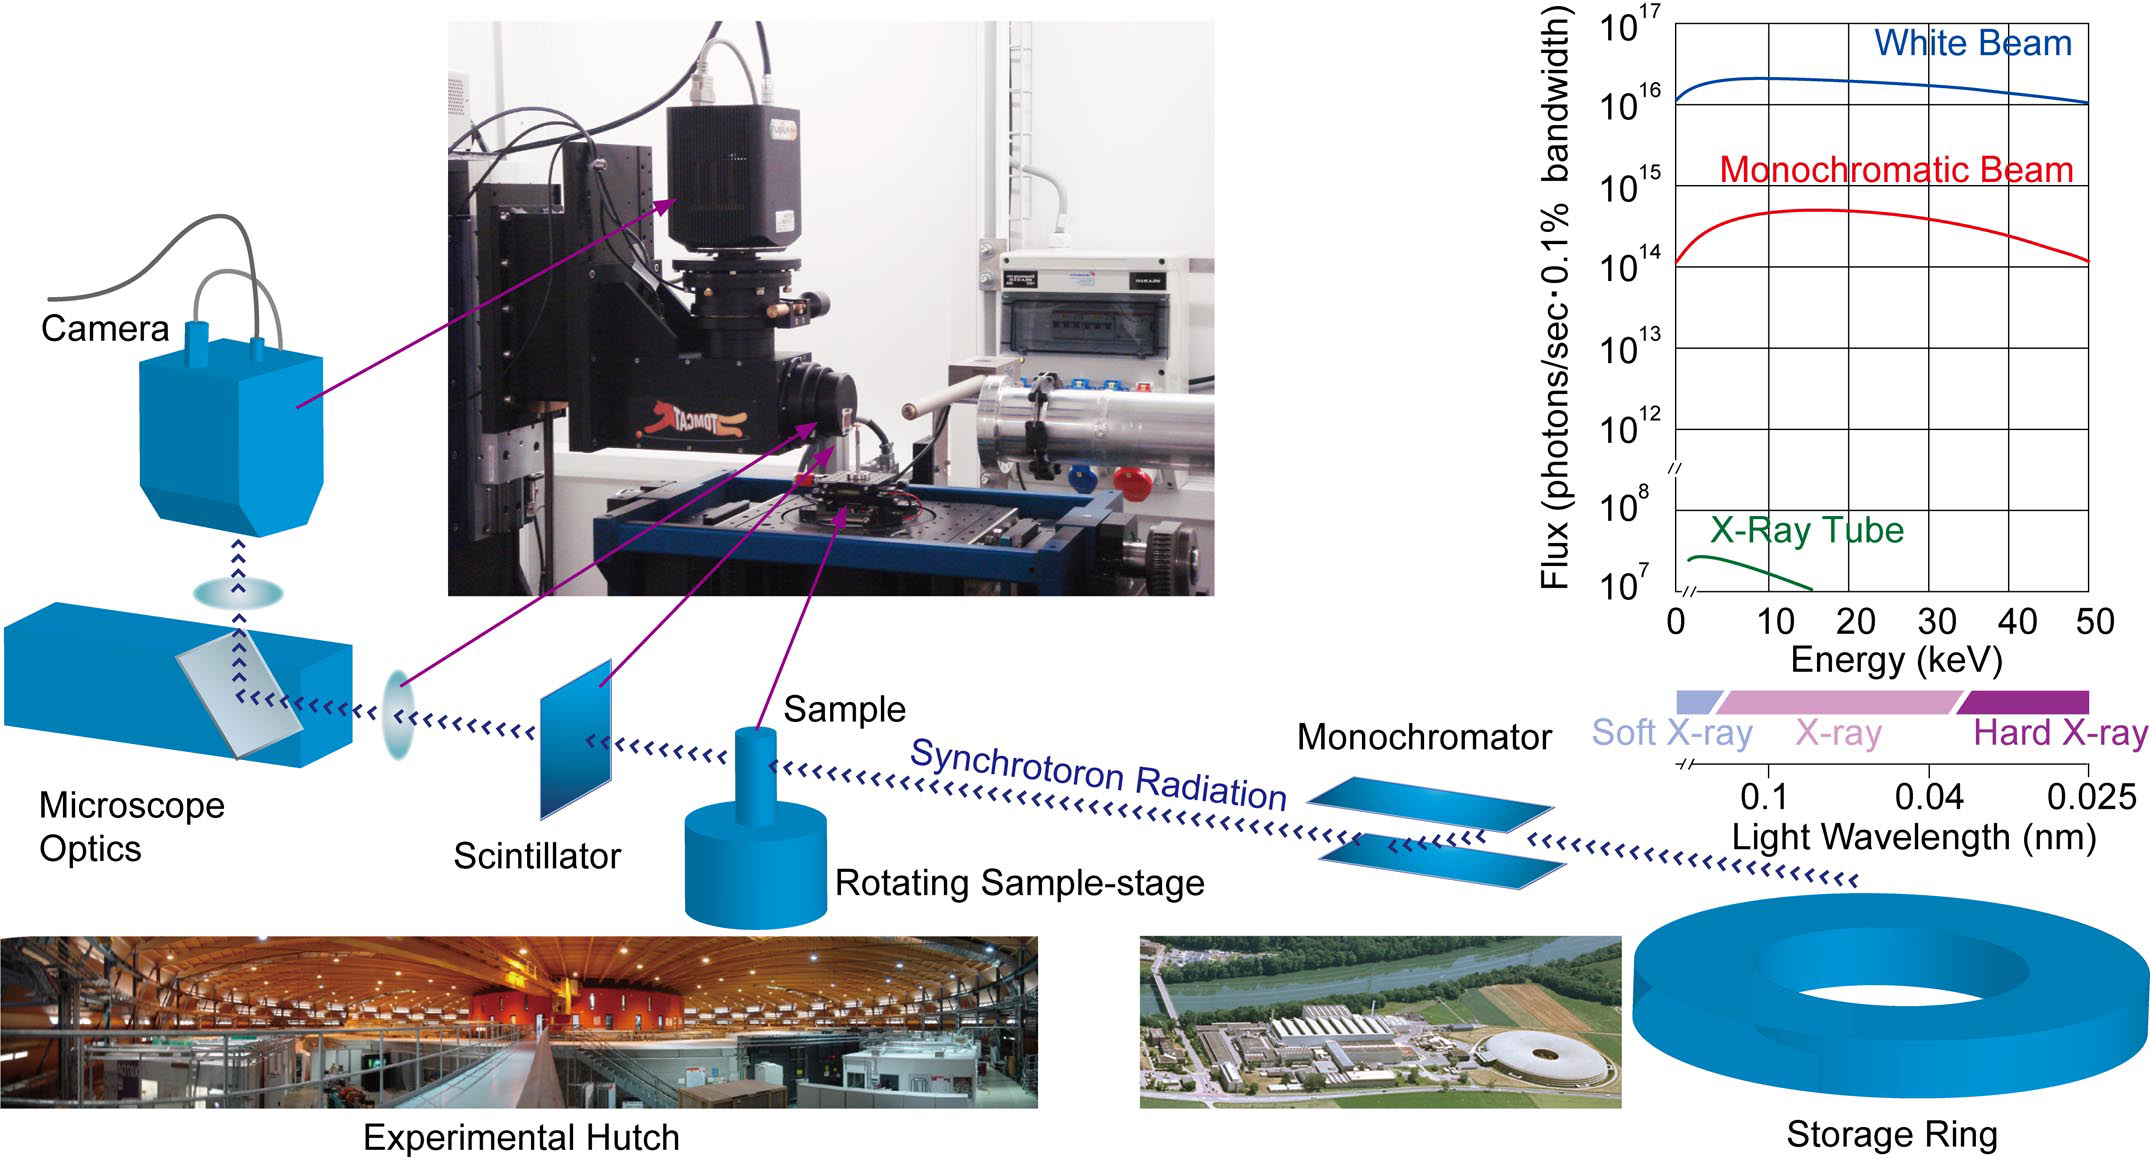
\includegraphics[width=\imsize]{img/Tsuda2008/Tsuda-02}
	\caption[SRXTM imaging setup]{Imaging setup. The X-rays are coupled out of the storage ring via a wiggler. The monochromator is then used to select a desired wavelength of the incident X-rays. The sample is placed on a rotating sample holder inside the beam. While the X-rays penetrate the sample, the stage is rotated, and in total 1500 projections over \SI{180}{\degree} are recorded. Plot shows spectrum of \ac{tomcat} (red and blue) compared with conventional X-ray tube (green).}
	\label{fig:imaging setup}
\end{figure}

\subsubsection{Image manipulation}
To facilitate detailed analysis for the development of \threed acinar reconstruction image processing, a cubic subregion of varying size was selected from the full dataset using the software Imaris (Bitplane, Zürich, Switzerland) installed on an Athlon 64 3500 based personal computer. Different subregions were chosen, typically representing a particular tissue structure, such as a cluster of alveoli without any large airways/branches, as well as a region without prominent ring artifacts. Ring artifacts represent an intrinsic problem of tomographic images and in our case are caused by very small particles trapped on the scintillator. They are usually limited to only some sections of the stack of images and are more prominent in the center of the sample. Before proceeding with the next step, we reduced the noise in some of the original \twod images and softened the image edges by using a Gaussian filter and/or a median filter with a 1$\times$3$\times$3 kernel.

\subsubsection{Segmentation: thresholding and binarization}
To render our samples in three dimensions, we first segmented the raw data. Segmentation is the process of classifying the voxels of an image. Each voxel must represent either air space or tissue, thus, all the different gray values of the individual voxels are binarized into either 0 (air space) or 1 (lung tissue). Guided by the histogram of the gray scale values of the raw image (not shown), we selected an initial, tentative threshold value. Because the final selection of the threshold level is one of the most crucial steps in segmentation, special care has been taken to determine a correct threshold.

As indicated in \autoref{fig:workflow}, we determined the appropriate threshold level iteratively: 
\begin{enumerate}
	\item we set an initial threshold level and performed segmentation;
	\item we sequentially performed the object-connectivity analysis and \threed reconstruction of objects (described below);
	\item we calculated and compared morphological parameters, such as volume density of tissue and surface area density of air space to those given by \citet{Tschanz2003}; and
	\item we readjusted/reset the threshold level based on the results of \textit{step 3} if necessary.
\end{enumerate}

We performed this iterative process until the calculated morphological parameters closely matched the values of the gold standard~\cite{Tschanz2003}.

\subsubsection{Object connectivity analysis}
Depending on the threshold level selected, erroneous holes and isolated small areas/objects may appear in the segmented images. To avoid these artifacts and to maintain object connectivity, we needed to preprocess the segmented voxels. We first determined the number of isolated objects and their sizes in the \ac{roi} and then eliminated the objects below a reasonable size ($\sim$5 pixels) by reclassifying voxel values (from ``airway'' to ``tissue'', or vice versa). This \ac{oca} was performed by implementing label adjacent pixel analysis in \threed \cite{Ballard1982,Davies1990,Gonzalez1992}. For the sake of simplicity and clarity, we will explain this algorithm in \twod as follows.

\def\scale{0.5}
\begin{figure}
	\centering
	\noindent\makebox[\textwidth]{%
		\subfloat[]{%
			% !TEX root = ../Thesis.tex
%\documentclass{article}
%\usepackage{tikz}
%\usepackage[graphics,tightpage,active]{preview}
%\PreviewEnvironment{tikzpicture}
%\begin{document}
%\def\scale{1}
%%%%%%%%%%%%%%%%%%%%%%%%%%%%%%%%%%%%%%%%%%%%%%%%%%%%%%%%%%%%%%
\begin{tikzpicture}[%
	scale=\scale,%
	number/.style ={white, text width=4em, text centered},%
	]
%%% grid
	\draw [thick] (0,0) -- (-.6,.6) node [anchor= south west] {Column} node [rotate=90,anchor= south east] {Row};
	\foreach \x in {0,...,11}
		{\draw (\x,0) -- (\x,-11);}
	\foreach \y in {0,...,-11}
		{\draw (0,\y) -- (11,\y);}
	\foreach \x in {1,...,11}
		\foreach \y in {0.5}
			{\draw (\x-.5,\y) node{\x};}
	\foreach \y/\label in {0/1,-1/2,-2/3,-3/4,-4/5,-5/6,-6/7,-7/8,-8/9,-9/10,-10/11}
		{\draw (-.5,\y-.5) node{\label};}
%%% grid
%%% fill
	\fill (1,-1) rectangle (2,-2);
	\fill (8,-2) rectangle (9,-3);
	\fill (2,-3) rectangle (4,-4);
	\fill (9,-3) rectangle (10,-4);
	\fill (5,-4) rectangle (6,-5);
	\fill (8,-4) rectangle (9,-5);
	\fill (4,-5) rectangle (8,-7);
	\fill (1,-7) rectangle (2,-9);
	\fill (4,-7) rectangle (7,-8);
	\fill (5,-8) rectangle (7,-9);
	%\fill (2,-9) rectangle (3,-10);
%%% fill
%%%% numbers
%	\node [number] at (1.5,-1.5) {1};
%	%
%	\node [number] at (8.5,-2.5) {2};
%	\node [number] at (9.5,-3.5) {2};
%	\node [number] at (9.5,-3.5) {2};
%	\node [number] at (8.5,-4.5) {\small 2/4};
%	%
%	\foreach \x in {2.5,3.5}
%		{\node [number] at (\x,-3.5) {3};}
%	%
%	\node [number] at (5.5,-4.5) {4};
%	\foreach \x in {4.5,...,6.5}
%	\foreach \y in {5.5,...,7.5}
%			{\node [number] at (\x,-\y) {4};}
%	\node [number] at (7.5,-5.5) {\small 4/2};
%	\node [number] at (7.5,-6.5) {4};
%	\foreach \x in {5.5,6.5}
%		{\node [number] at (\x,-8.5) {4};}
%	%
%	\foreach \y in {7.5,8.5}
%		{\node [number] at (1.5,-\y) {5};}
%	\node [number] at (2.5,-9.5) {5};
%%%% numbers
\end{tikzpicture}
%%%%%%%%%%%%%%%%%%%%%%%%%%%%%%%%%%%%%%%%%%%%%%%%%%%%%%%%%%%%%%
%\end{document}%
			\label{subfig:tsuda-03a}%
		}%
		\subfloat[]{%
			% !TEX root = ../Thesis.tex
%\documentclass{article}
%\usepackage{tikz}
%\usepackage[graphics,tightpage,active]{preview}
%\PreviewEnvironment{tikzpicture}
%\begin{document}
%\def\scale{1}
%%%%%%%%%%%%%%%%%%%%%%%%%%%%%%%%%%%%%%%%%%%%%%%%%%%%%%%%%%%%%%
\begin{tikzpicture}[%
	scale=\scale,%
	number/.style ={white, text width=4em, text centered},%
	]
%%% grid
	\draw [thick] (0,0) -- (-.6,.6) node [anchor= south west] {Column} node [rotate=90,anchor= south east] {Row};
	\foreach \x in {0,...,11}
		{\draw (\x,0) -- (\x,-11);}
	\foreach \y in {0,...,-11}
		{\draw (0,\y) -- (11,\y);}
	\foreach \x in {1,...,11}
		\foreach \y in {0.5}
			{\draw (\x-.5,\y) node{\x};}
	\foreach \y/\label in {0/1,-1/2,-2/3,-3/4,-4/5,-5/6,-6/7,-7/8,-8/9,-9/10,-10/11}
		{\draw (-.5,\y-.5) node{\label};}
%%% grid
%%% fill
	\fill (1,-1) rectangle (2,-2);
	\fill (8,-2) rectangle (9,-3);
	\fill (2,-3) rectangle (4,-4);
	\fill (9,-3) rectangle (10,-4);
	\fill (5,-4) rectangle (6,-5);
	\fill (8,-4) rectangle (9,-5);
	\fill (4,-5) rectangle (8,-7);
	\fill (1,-7) rectangle (2,-9);
	\fill (4,-7) rectangle (7,-8);
	\fill (5,-8) rectangle (7,-9);
	\fill (2,-9) rectangle (3,-10);
%%% fill
%%%% numbers
	\node [number] at (1.5,-1.5) {1};
	%
	\node [number] at (8.5,-2.5) {2};
	\node [number] at (9.5,-3.5) {2};
	\node [number] at (9.5,-3.5) {2};
	\node [number,color=red] at (8.5,-4.5) {\scriptsize 2/4};
	%
	\foreach \x in {2.5,3.5}
		{\node [number] at (\x,-3.5) {3};}
	%
	\node [number] at (5.5,-4.5) {4};
	\foreach \x in {4.5,...,6.5}
	\foreach \y in {5.5,...,7.5}
			{\node [number] at (\x,-\y) {4};}
	\node [number,color=red] at (7.5,-5.5) {\scriptsize 4/2};
	\node [number] at (7.5,-6.5) {4};
	\foreach \x in {5.5,6.5}
		{\node [number] at (\x,-8.5) {4};}
	%
	\foreach \y in {7.5,8.5}
		{\node [number] at (1.5,-\y) {5};}
	\node [number] at (2.5,-9.5) {5};
%%%% numbers
\end{tikzpicture}
%%%%%%%%%%%%%%%%%%%%%%%%%%%%%%%%%%%%%%%%%%%%%%%%%%%%%%%%%%%%%%
%\end{document}%
			\label{subfig:tsuda-03b}%
		}%
	}\\% end makebox
	\noindent\makebox[\textwidth]{%
		\subfloat[]{%
			% !TEX root = ../Thesis.tex
%\documentclass{article}
%\usepackage{tikz}
%\usepackage[graphics,tightpage,active]{preview}
%\PreviewEnvironment{tikzpicture}
%\begin{document}
%\def\scale{1}
%%%%%%%%%%%%%%%%%%%%%%%%%%%%%%%%%%%%%%%%%%%%%%%%%%%%%%%%%%%%%%
\begin{tikzpicture}[%
	scale=\scale,%
	number/.style ={black, text width=4em, text centered},%
	]
%%% grid
	\draw [thick] (0,0) -- (-.6,.6) node [anchor= south west] {Column} node [rotate=90,anchor= south east] {Row};
	\foreach \x in {0,...,11}
		{\draw (\x,0) -- (\x,-11);}
	\foreach \y in {0,...,-11}
		{\draw (0,\y) -- (11,\y);}
	\foreach \x in {1,...,11}
		\foreach \y in {0.5}
			{\draw (\x-.5,\y) node{\x};}
	\foreach \y/\label in {0/1,-1/2,-2/3,-3/4,-4/5,-5/6,-6/7,-7/8,-8/9,-9/10,-10/11}
		{\draw (-.5,\y-.5) node{\label};}
%%% grid
%%% fill
%	\fill (1,-1) rectangle (2,-2);
%	\fill (8,-2) rectangle (9,-3);
%	\fill (2,-3) rectangle (4,-4);
%	\fill (9,-3) rectangle (10,-4);
%	\fill (5,-4) rectangle (6,-5);
%	\fill (8,-4) rectangle (9,-5);
%	\fill (4,-5) rectangle (8,-7);
%	\fill (1,-7) rectangle (2,-9);
%	\fill (4,-7) rectangle (7,-8);
%	\fill (5,-8) rectangle (7,-9);
%	\fill (2,-9) rectangle (3,-10);
%%% fill
%%%% numbers
	\node [number] at (1.5,-1.5) {1};
	%
	\node [number] at (8.5,-2.5) {4};
	\node [number] at (9.5,-3.5) {4};
	\node [number] at (9.5,-3.5) {4};
	\node [number] at (8.5,-4.5) {4};
	%
	\foreach \x in {2.5,3.5}
		{\node [number] at (\x,-3.5) {3};}
	%
	\node [number] at (5.5,-4.5) {4};
	\foreach \x in {4.5,...,6.5}
	\foreach \y in {5.5,...,7.5}
			{\node [number] at (\x,-\y) {4};}
	\node [number] at (7.5,-5.5) {4};
	\node [number] at (7.5,-6.5) {4};
	\foreach \x in {5.5,6.5}
		{\node [number] at (\x,-8.5) {4};}
	%
	\foreach \y in {7.5,8.5}
		{\node [number] at (1.5,-\y) {5};}
	\node [number] at (2.5,-9.5) {5};
%%%% numbers
\end{tikzpicture}
%%%%%%%%%%%%%%%%%%%%%%%%%%%%%%%%%%%%%%%%%%%%%%%%%%%%%%%%%%%%%%
%\end{document}%
			\label{subfig:tsuda-03c}%
		}%
		\subfloat[]{%
			% !TEX root = ../Thesis.tex
%\documentclass{article}
%\usepackage{tikz}
%\usepackage[graphics,tightpage,active]{preview}
%\PreviewEnvironment{tikzpicture}
%\begin{document}
%\def\scale{1}
%%%%%%%%%%%%%%%%%%%%%%%%%%%%%%%%%%%%%%%%%%%%%%%%%%%%%%%%%%%%%%
\begin{tikzpicture}[%
	scale=\scale,%
	number/.style ={white, text width=4em, text centered},%
	]
%%% fill
	\fill [fill=lightgray] (1,-1) rectangle (2,-2);
	\fill (8,-2) rectangle (9,-3);
	\fill [fill=lightgray] (2,-3) rectangle (4,-4);
	\fill (9,-3) rectangle (10,-4);
	\fill (5,-4) rectangle (6,-5);
	\fill (8,-4) rectangle (9,-5);
	\fill (4,-5) rectangle (8,-7);
	\fill [fill=lightgray] (1,-7) rectangle (2,-9);
	\fill (4,-7) rectangle (7,-8);
	\fill (5,-8) rectangle (7,-9);
	\fill [fill=lightgray] (2,-9) rectangle (3,-10);
%%% fill
%%% grid
	\draw [thick] (0,0) -- (-.6,.6) node [anchor= south west] {Column} node [rotate=90,anchor= south east] {Row};
	\foreach \x in {0,...,11}
		{\draw (\x,0) -- (\x,-11);}
	\foreach \y in {0,...,-11}
		{\draw (0,\y) -- (11,\y);}
	\foreach \x in {1,...,11}
		\foreach \y in {0.5}
			{\draw (\x-.5,\y) node{\x};}
	\foreach \y/\label in {0/1,-1/2,-2/3,-3/4,-4/5,-5/6,-6/7,-7/8,-8/9,-9/10,-10/11}
		{\draw (-.5,\y-.5) node{\label};}
%%% grid
%%%% numbers
%	\node [number] at (1.5,-1.5) {1};
%	%
%	\node [number] at (8.5,-2.5) {2};
%	\node [number] at (9.5,-3.5) {2};
%	\node [number] at (9.5,-3.5) {2};
%	\node [number] at (8.5,-4.5) {\small 2/4};
%	%
%	\foreach \x in {2.5,3.5}
%		{\node [number] at (\x,-3.5) {3};}
%	%
%	\node [number] at (5.5,-4.5) {4};
%	\foreach \x in {4.5,...,6.5}
%	\foreach \y in {5.5,...,7.5}
%			{\node [number] at (\x,-\y) {4};}
%	\node [number] at (7.5,-5.5) {\small 4/2};
%	\node [number] at (7.5,-6.5) {4};
%	\foreach \x in {5.5,6.5}
%		{\node [number] at (\x,-8.5) {4};}
%	%
%	\foreach \y in {7.5,8.5}
%		{\node [number] at (1.5,-\y) {5};}
%	\node [number] at (2.5,-9.5) {5};
%%%% numbers
\end{tikzpicture}
%%%%%%%%%%%%%%%%%%%%%%%%%%%%%%%%%%%%%%%%%%%%%%%%%%%%%%%%%%%%%%
%\end{document}%
			\label{subfig:tsuda-03d}%
		}%
	}%
	\caption[Object connectivity analysis]{Object connectivity analysis shown in a 2-dimensional (\twod) example. \subref{subfig:tsuda-03a}: a binary distribution of ``black'' vs.\ ``white'' pixels at certain threshold level; \subref{subfig:tsuda-03b}: An object label number (\acs{oln}) is assigned for each black pixel on the basis of the color (black or white) of 4 adjacent pixels; \subref{subfig:tsuda-03c}: on the basis of a ``flag'' pixel (red text in panel \subref{subfig:tsuda-03b}), connectivity is identified between \ac{oln}=2 and \ac{oln}=4; \subref{subfig:tsuda-03d}: small objects less than cutoff (=4 pixels in this example, light gray) are removed.}
	\label{fig:tsuda-03}
\end{figure}

Let us assume that ``black'' and ``white'' pixels (voxels in a \threed case) are distributed as in the example shown in \autoref{subfig:tsuda-03a}. Scanning pixels from top to bottom and from left to right, we will examine the connectivity of each black pixel, by checking the colors (black or white) of its four adjacent pixels [a pixel on its left and three pixels on its top (top left, top middle, top right)]. We will assign a tentative \acf{oln} (consecutively, 1, 2, 3, 4\ldots) to each black pixel and examine connections between identified objects. Four simple logical algorithms are involved.
\begin{enumerate}
	\item If all four adjacent pixels are white, assign a new \ac{oln} to the current black pixel. [For instance, we assign \ac{oln}=1 to the pixel at (column 2; row 2); \ac{oln}=2 to the pixel at (9;3), etc. (\autoref{subfig:tsuda-03b}).]
	\item If only one of the adjacent pixels has already been assigned an \ac{oln}, assign the same \ac{oln} to the current black pixel. [For instance, we assign the \ac{oln}=3 to the pixel at (4;4) because the adjacent pixel on the left of it (at 3;4) has already been assigned with \ac{oln}=3 (\autoref{subfig:tsuda-03b}).]
	\item If more than one adjacent pixels have already been assigned an \ac{oln} and if those adjacent pixels have the same \ac{oln}, assign the same \ac{oln} to the current pixel. [For instance, we assign \ac{oln}=4 to the pixel at (6;6) because the adjacent pixels at (5;6) and at (6;5) have already been assigned with an \ac{oln}=4 (\autoref{subfig:tsuda-03b}).]
	\item If more than one adjacent pixel has already been assigned an \ac{oln} but if those adjacent pixels have different \acp{oln}, assign one of the adjacent pixel's \ac{oln} and put a special marker (flag) on that pixel. The pixel with this flag will be re-examined in the next step. [For instance, we assign either \ac{oln}=2 or 4 to the pixel at (8;6) because the adjacent pixels at (9;5) and at (7;6) have already been assigned with \ac{oln}=2 and 4, respectively. Thus, the pixel is marked with a flag (shown red in \autoref{subfig:tsuda-03b}).]
\end{enumerate}
After assigning \acp{oln} to all the black pixels, we then re-examine the flagged pixels, which indicate that two or more ``appeared-to-be separated'' objects are indeed connected. We reassign the same \ac{oln} to all of the connected pixels leaving from the flagged pixel. For instance, we assigned \ac{oln}=4 to the pixel at (8;6). This means that the pixels (9; 3), (10; 4) and (9; 5) are also assigned with the \ac{oln}=4 (\autoref{subfig:tsuda-03c}). Finally, we remove small objects that are physically unreasonable in size ($<$5 pixels; \autoref{subfig:tsuda-03d}), suppressing noise and artifacts from the image acquisition.

\subsubsection{\threed reconstruction of separated objects}
Much of the currently available medical imaging software for \threed reconstruction treats objects (\ie, lung tissues in our case) as surfaces, and this is most often done by a triangulation of the voxel surface. However, to perform a complete \threed reconstruction, we use a different approach here; we reconstruct not only the surface of the boundary between the tissue and the air space, but also the volumes of tissues and air space by fitting \ac{fe} to the raw voxel data and hence inside the full volume. For this, we use a \ac{gbha}~\cite{Schneiders1996}, which is explained as follows.

Let us consider an example in which we want to apply a threshold of 123 for the segmentation of our images. In \autoref{subfig:tsuda-04a}, at \textit{left} the thresholded voxels in a \threed representation is shown and, for the sake of discussion and clarity, a \twod representation is shown at \textit{right}.
\begin{description}
	\item[1. Mesh generation] A \ac{fe} mesh (\autoref{subfig:tsuda-04b}), initially uniform, is isotropically generated over all pixels. We position the nodes of the \ac{fe} mesh at the centers of the existing voxels (\autoref{subfig:tsuda-04b}, \textit{right}). This means that each \ac{fe} overlaps 2$\times$2 voxels in the \twod case. (\autoref{subfig:tsuda-04b}, \textit{right}) or 2$\times$2$\times$2 voxels in the \threed case (\autoref{subfig:tsuda-04b}, \textit{left}). The black circles represent nodes generated inside the object and the white circles denote nodes outside of the object. The nodes inside the object have a pixel or voxel value higher than the chosen threshold and the nodes outside the object have a value lower than the chosen threshold. Each \ac{fe} node is assigned the grayscale value of the corresponding voxel. Note that the boundary between the black and white nodes is not smooth at this stage.
	\item[2. Surface smoothing I] Because the \ac{fe} mesh is located on the surface boundary, some of its nodes (shown as the white circles) are on the outside of the object. Additionally, the grayscale pixel values of those white nodes are lower than the chosen threshold value. By using a simple linear interpolation, we move these white nodes in the direction of the surface boundary toward the locations where the grayscale pixel value would exactly match the threshold value. There are multiple methods available to move the nodes by linear interpolation. We adapted the method developed by \citet{Schneiders1996} for our \threed case. It is important to note that in some cases, this linear interpolation might even move the node inside the object (see \autoref{subfig:tsuda-04c} for examples).
	\item[3. Surface smoothing II] The translation of the nodes as described in \textit{step 2} may in some cases lead to a distorted (concave) \ac{fe} surface. The distortion of the \ac{fe} nodes can be evaluated with their Jacobian value. The Jacobian value is a matrix of the derivation of global to local \ac{fe} interpolation function and the quality of any mesh can be directly evaluated by its Jacobian value~\cite{Bathe1995}. Distorted \acp{fe}, which are not suitable for subsequent numerical calculations, show a negative Jacobian. To optimize the Jacobian, we implemented the standard \ac{lst}~\cite{Freitag2000}). The \ac{lst} usually takes a few loops (repetitions of \textit{step 2}) over all \acp{fe} to achieve positive Jacobian values for all \acp{fe}. The results of applying the \ac{lst} for \threed and \twod cases are shown, respectively, in \autoref{subfig:tsuda-04d}, \textit{right} (``After \ac{lst}'').
\end{description}

\renewcommand{\imsize}{\linewidth}
\begin{figure}
	\centering
	\subfloat[]{%
		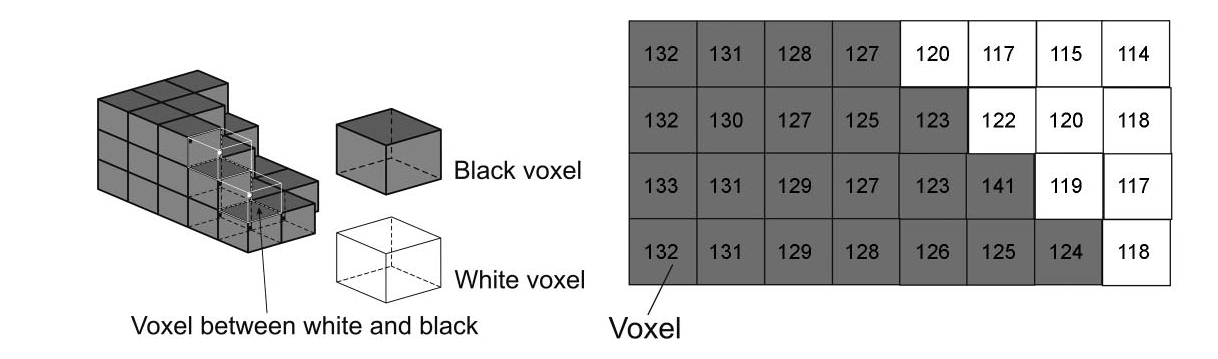
\includegraphics[width=\imsize]{img/Tsuda2008/Tsuda-04a}%
		\label{subfig:tsuda-04a}%
	}\\%
	\subfloat[]{%
		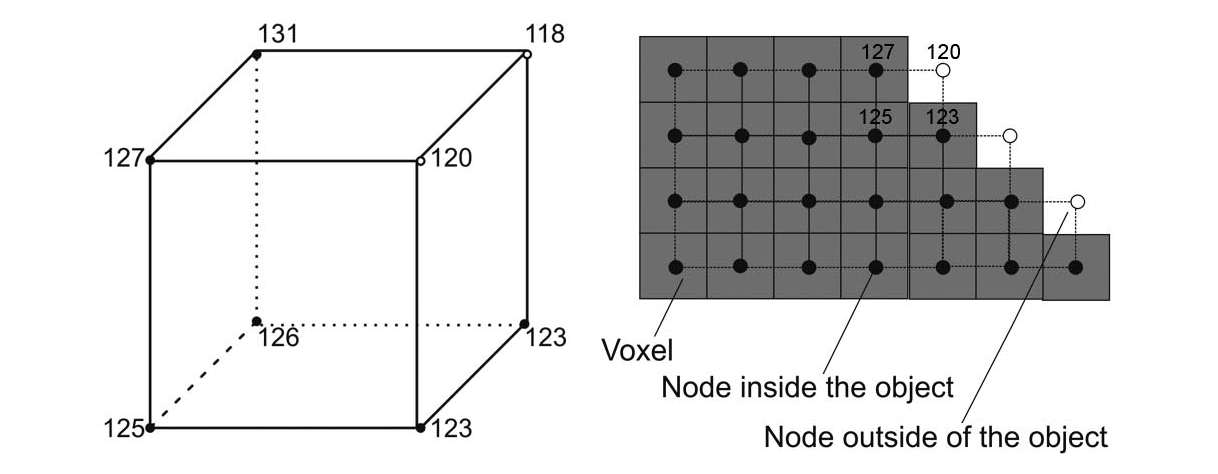
\includegraphics[width=\imsize]{img/Tsuda2008/Tsuda-04b}%
		\label{subfig:tsuda-04b}%
	}\\%
	\subfloat[]{%
		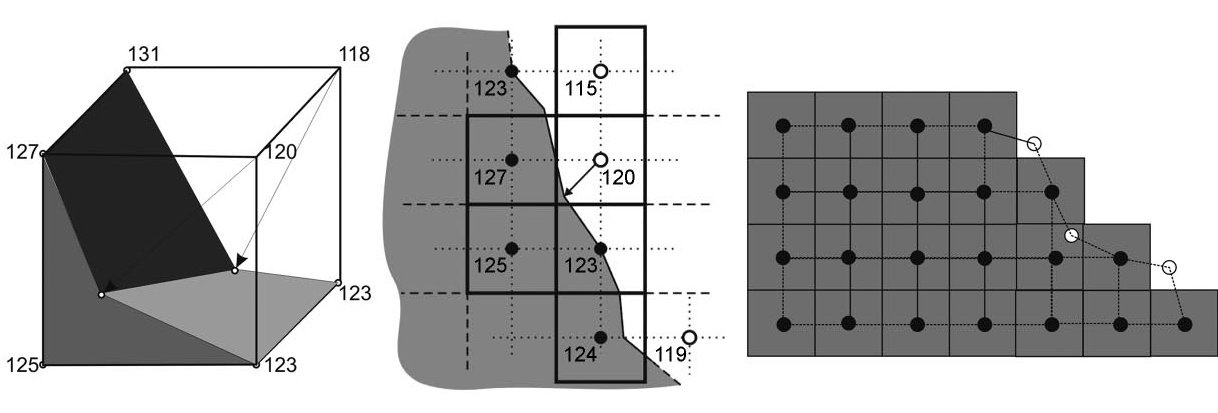
\includegraphics[width=\imsize]{img/Tsuda2008/Tsuda-04c}%
		\label{subfig:tsuda-04c}%
	}\\%
	\subfloat[]{%
		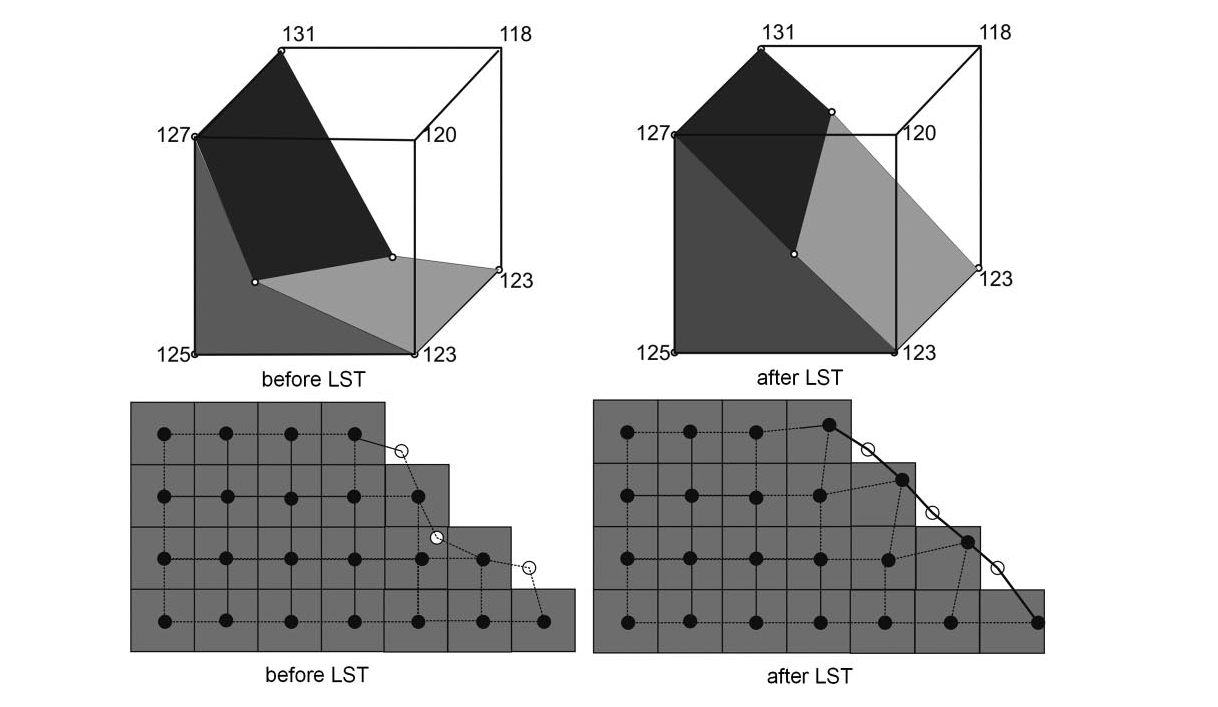
\includegraphics[width=\imsize]{img/Tsuda2008/Tsuda-04d}%
		\label{subfig:tsuda-04d}%
	}%
	\caption[Grid-based hexahedral algorithm]{Grid-based hexahedral algorithm. \subref{subfig:tsuda-04a}: \threed thresholded voxels (\textit{left}) and \twod representation of thresholded voxels (\textit{right}). The grayscale values are kept in the map of voxel. \subref{subfig:tsuda-04b}: step 1: generation of uniform \acl{fe} mesh over the voxel map. For simplicity, \ac{fe} nodes are positioned at the center of voxel. \threed \ac{fe} meshing (\textit{left}) and \twod \ac{fe} meshing (\textit{right}) are shown. Each node is assigned with the grayscale value from the corresponding voxel. \subref{subfig:tsuda-04c}: step 2: moving nodes on the surface due to trilinear interpolation in \threed case (\textit{left}) and bilinear interpolation in \twod case (\textit{right}). The location of surface boundary is shown in the middle image for \twod case. A fast sub \ac{fe}-voxel level algorithm is implemented to locate a surface boundary. White nodes are moving toward this surface boundary. \subref{subfig:tsuda-04d}: step 3: \acf{lst}. \threed and \twod before \ac{lst} (\textit{left}), \threed and \twod after \ac{lst} (\textit{right}).}
	\label{fig:tsuda-04}
\end{figure}

\subsection[Validation of Segmentation]{Validation of Segmentation and Image Processing}
Once \threed reconstruction was performed with a certain tentative threshold value, the resulting \threed structure was evaluated against the gold standard, \ie, well-characterized morphometric data provided by \citet{Tschanz2003}. We calculated the volume density of tissue (V\textsubscript{VS}) and surface area density of air space (S\textsubscript{VS}~[\centimetresquared\per\centimetrecubed]) to determine if there was unacceptable discrepancy. If so, we readjusted the threshold level and repeated the segmentation process, mesh generation, and subsequent image analysis until our calculated morphological parameters were within $<$\SI{5}{\percent} difference of the gold standard (\autoref{fig:workflow}).

\subsection[Visualization of the Reconstruction]{Visualization of the \threed Reconstruction}
Once the calculated morphological parameters met the gold standard, the resulting \threed reconstruction was transformed in a standard \acs{vrml} format for visualization as well as a proprietary DAT format for subsequent \ac{fe} analysis.

\section{Results}
The Epon embedded lung tissue samples of a 60-day-old rat were selected from the ``lung tissue library'' of Peter Burri's lab (University of Bern). All morphological parameters of this particular rat, against which our data were compared, are available and published in~\citet{Tschanz2003}.

\subsection{A Raw Image Stack and a Cubic Subregion}
The samples were scanned with \ac{srxtm} and a stack of 1024 raw images was reconstructed in tiff format (\autoref{subfig:tsuda-05a}: stack of images, \ref{subfig:tsuda-05b}: one slice of the raw data). The resolution of the image was \SI{1.4}{\micro\meter} per pixel, thus the edge length of the cubic stack was \SI{1.4336}{\milli\meter}, containing approximately one billion isotropic voxels.

To facilitate further processing of the image, different subregions of interest were extracted from the original raw data (one exemplary \ac{roi} is the orange small cube in \autoref{subfig:tsuda-05a}, which is shown enlarged in \autoref{subfig:tsuda-05c}. This \ac{roi} has a size of 196$\times$196$\times$196 pixels (\ie, an edge length of $\sim$\SI{275}{\micro\meter}) and contains $\sim$7.5 million voxels. This is a reasonable size of data that can easily be handled by a standard \acsu{pc} (Duo Core 2 Pentium \SI{2.33}{\gigahertz}, \SI{2}{\giga\byte} \acs{ram}) for visualization and volume rendering. The aforementioned size is an intermediate \ac{roi}; depending on the need for visualization/volume rendering other sizes have been chosen. To validate the segmentation (see below), we split a big \ac{roi} inside the sample in the full dataset vertically into five subregions leading to a \ac{roi} size of 200$\times$200$\times$180 pixels.

\renewcommand{\imsize}{0.5\linewidth}
\begin{figure}[h]
	\centering
	\subfloat[]{%
		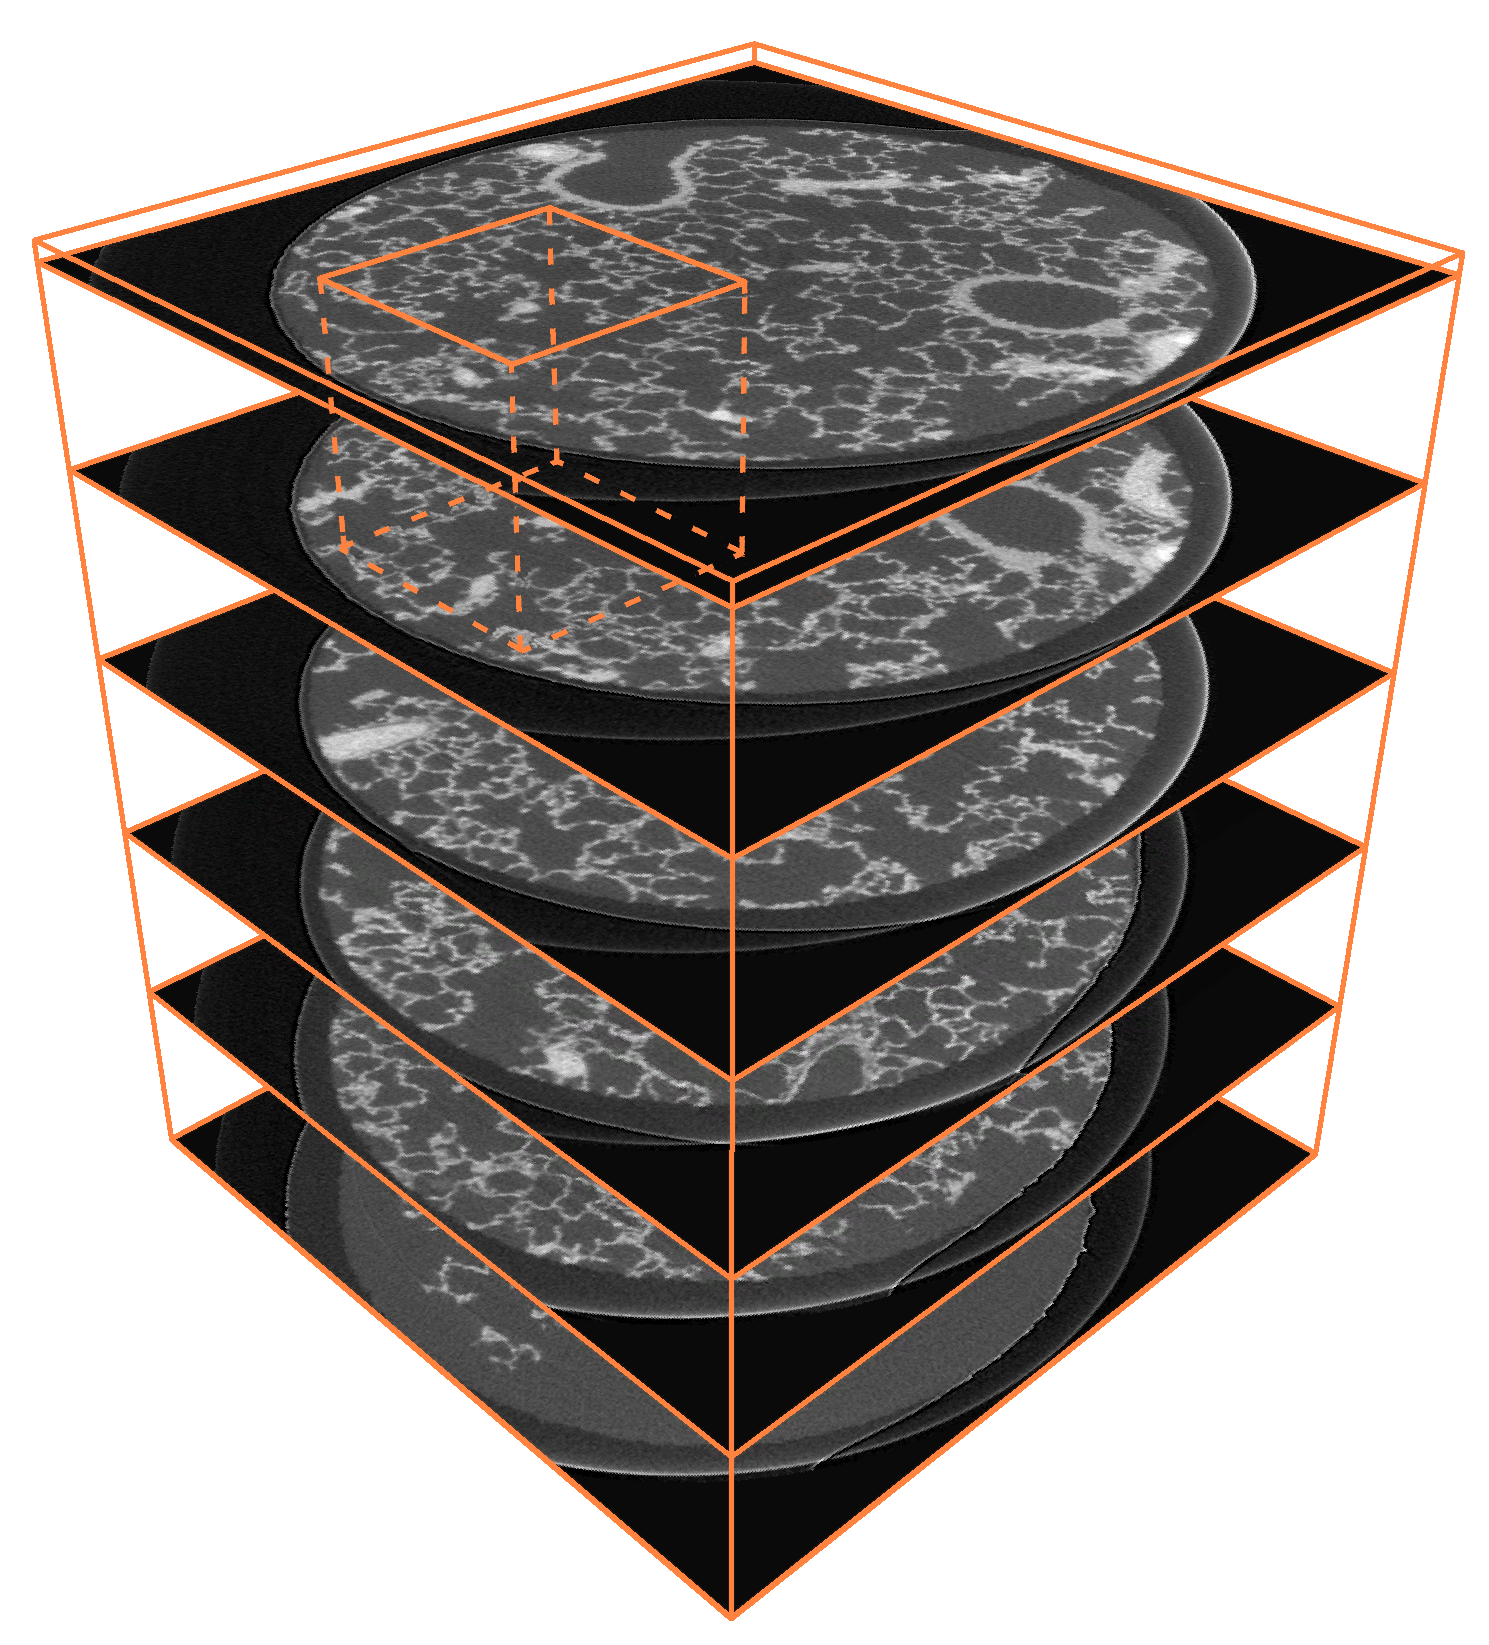
\includegraphics[width=\imsize]{img/Tsuda2008/Tsuda-05a}%
		\label{subfig:tsuda-05a}%
	}\hfill%
	\subfloat[]{%
		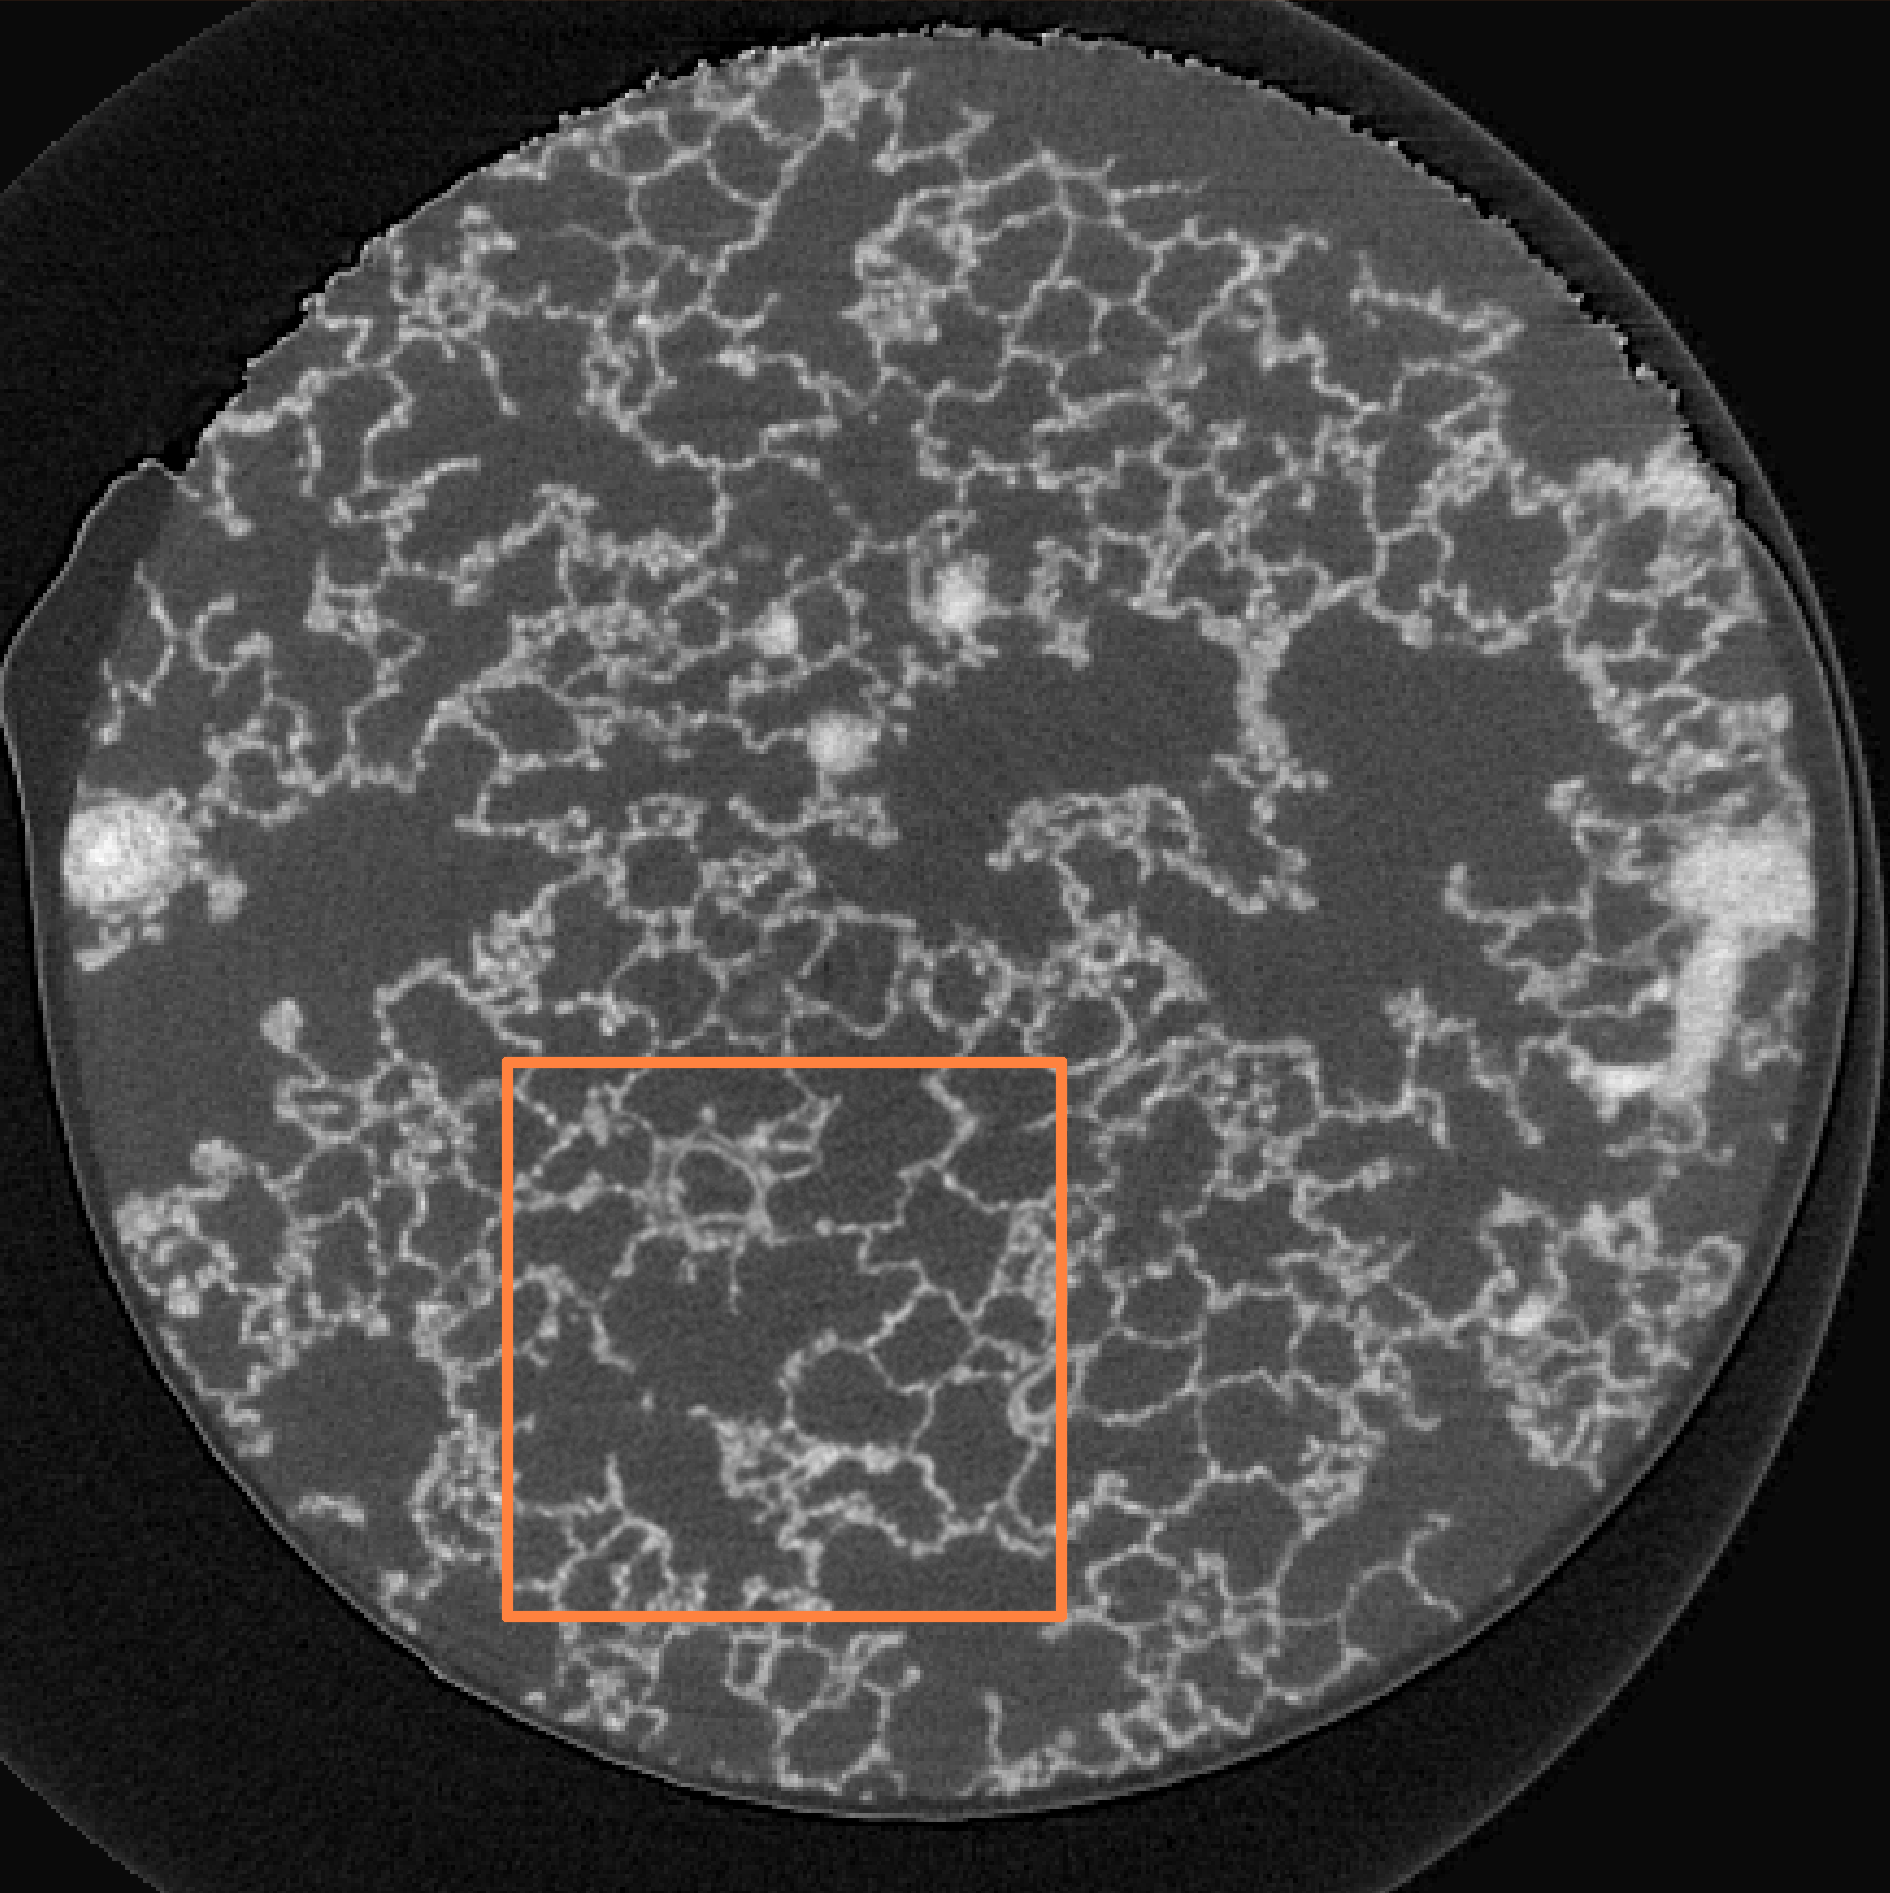
\includegraphics[width=\imsize]{img/Tsuda2008/Tsuda-05b}%
		\label{subfig:tsuda-05b}%
	}\\%
	\subfloat[]{%
		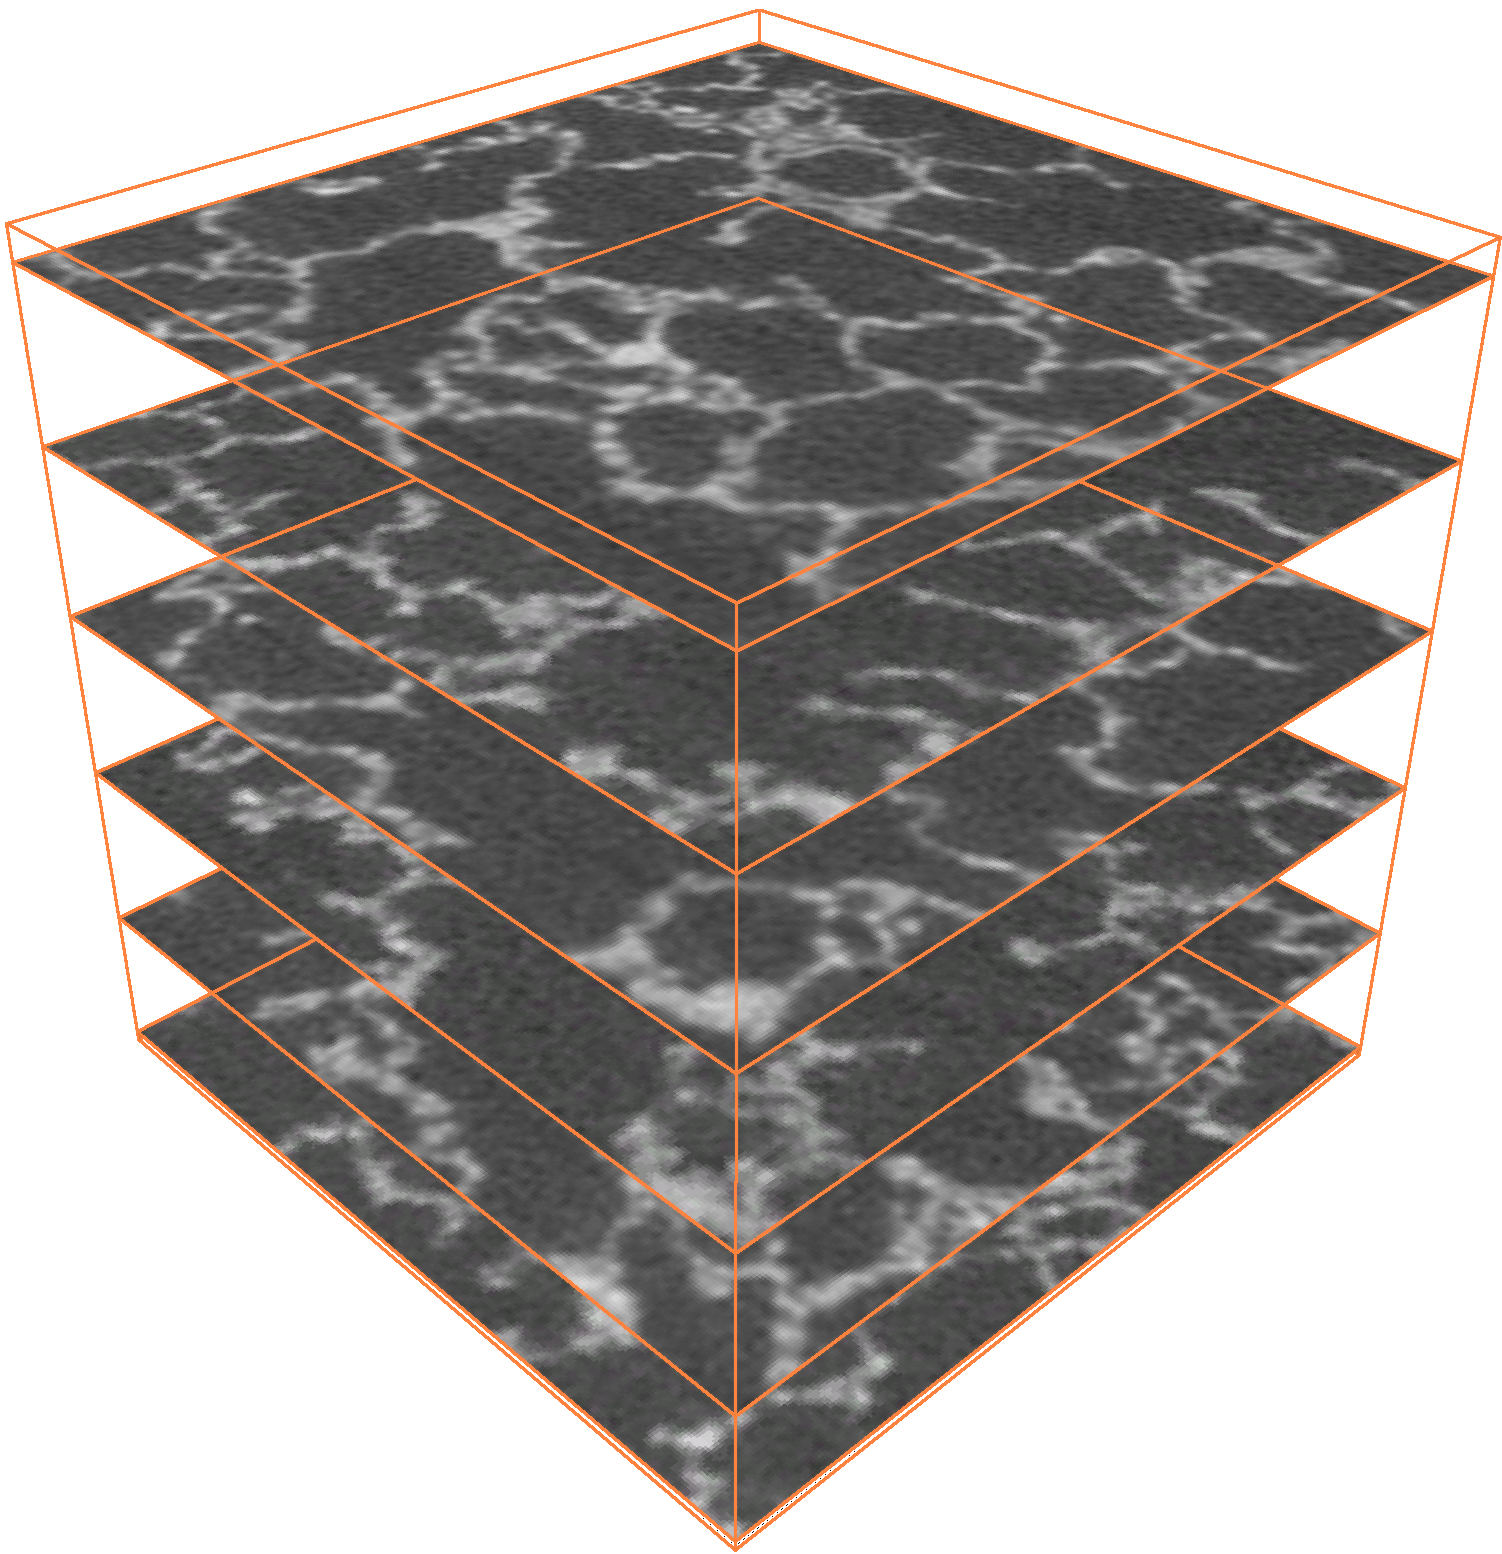
\includegraphics[width=\imsize]{img/Tsuda2008/Tsuda-05c}%
		\label{subfig:tsuda-05c}%
	}\hfill%
	\subfloat[]{%
		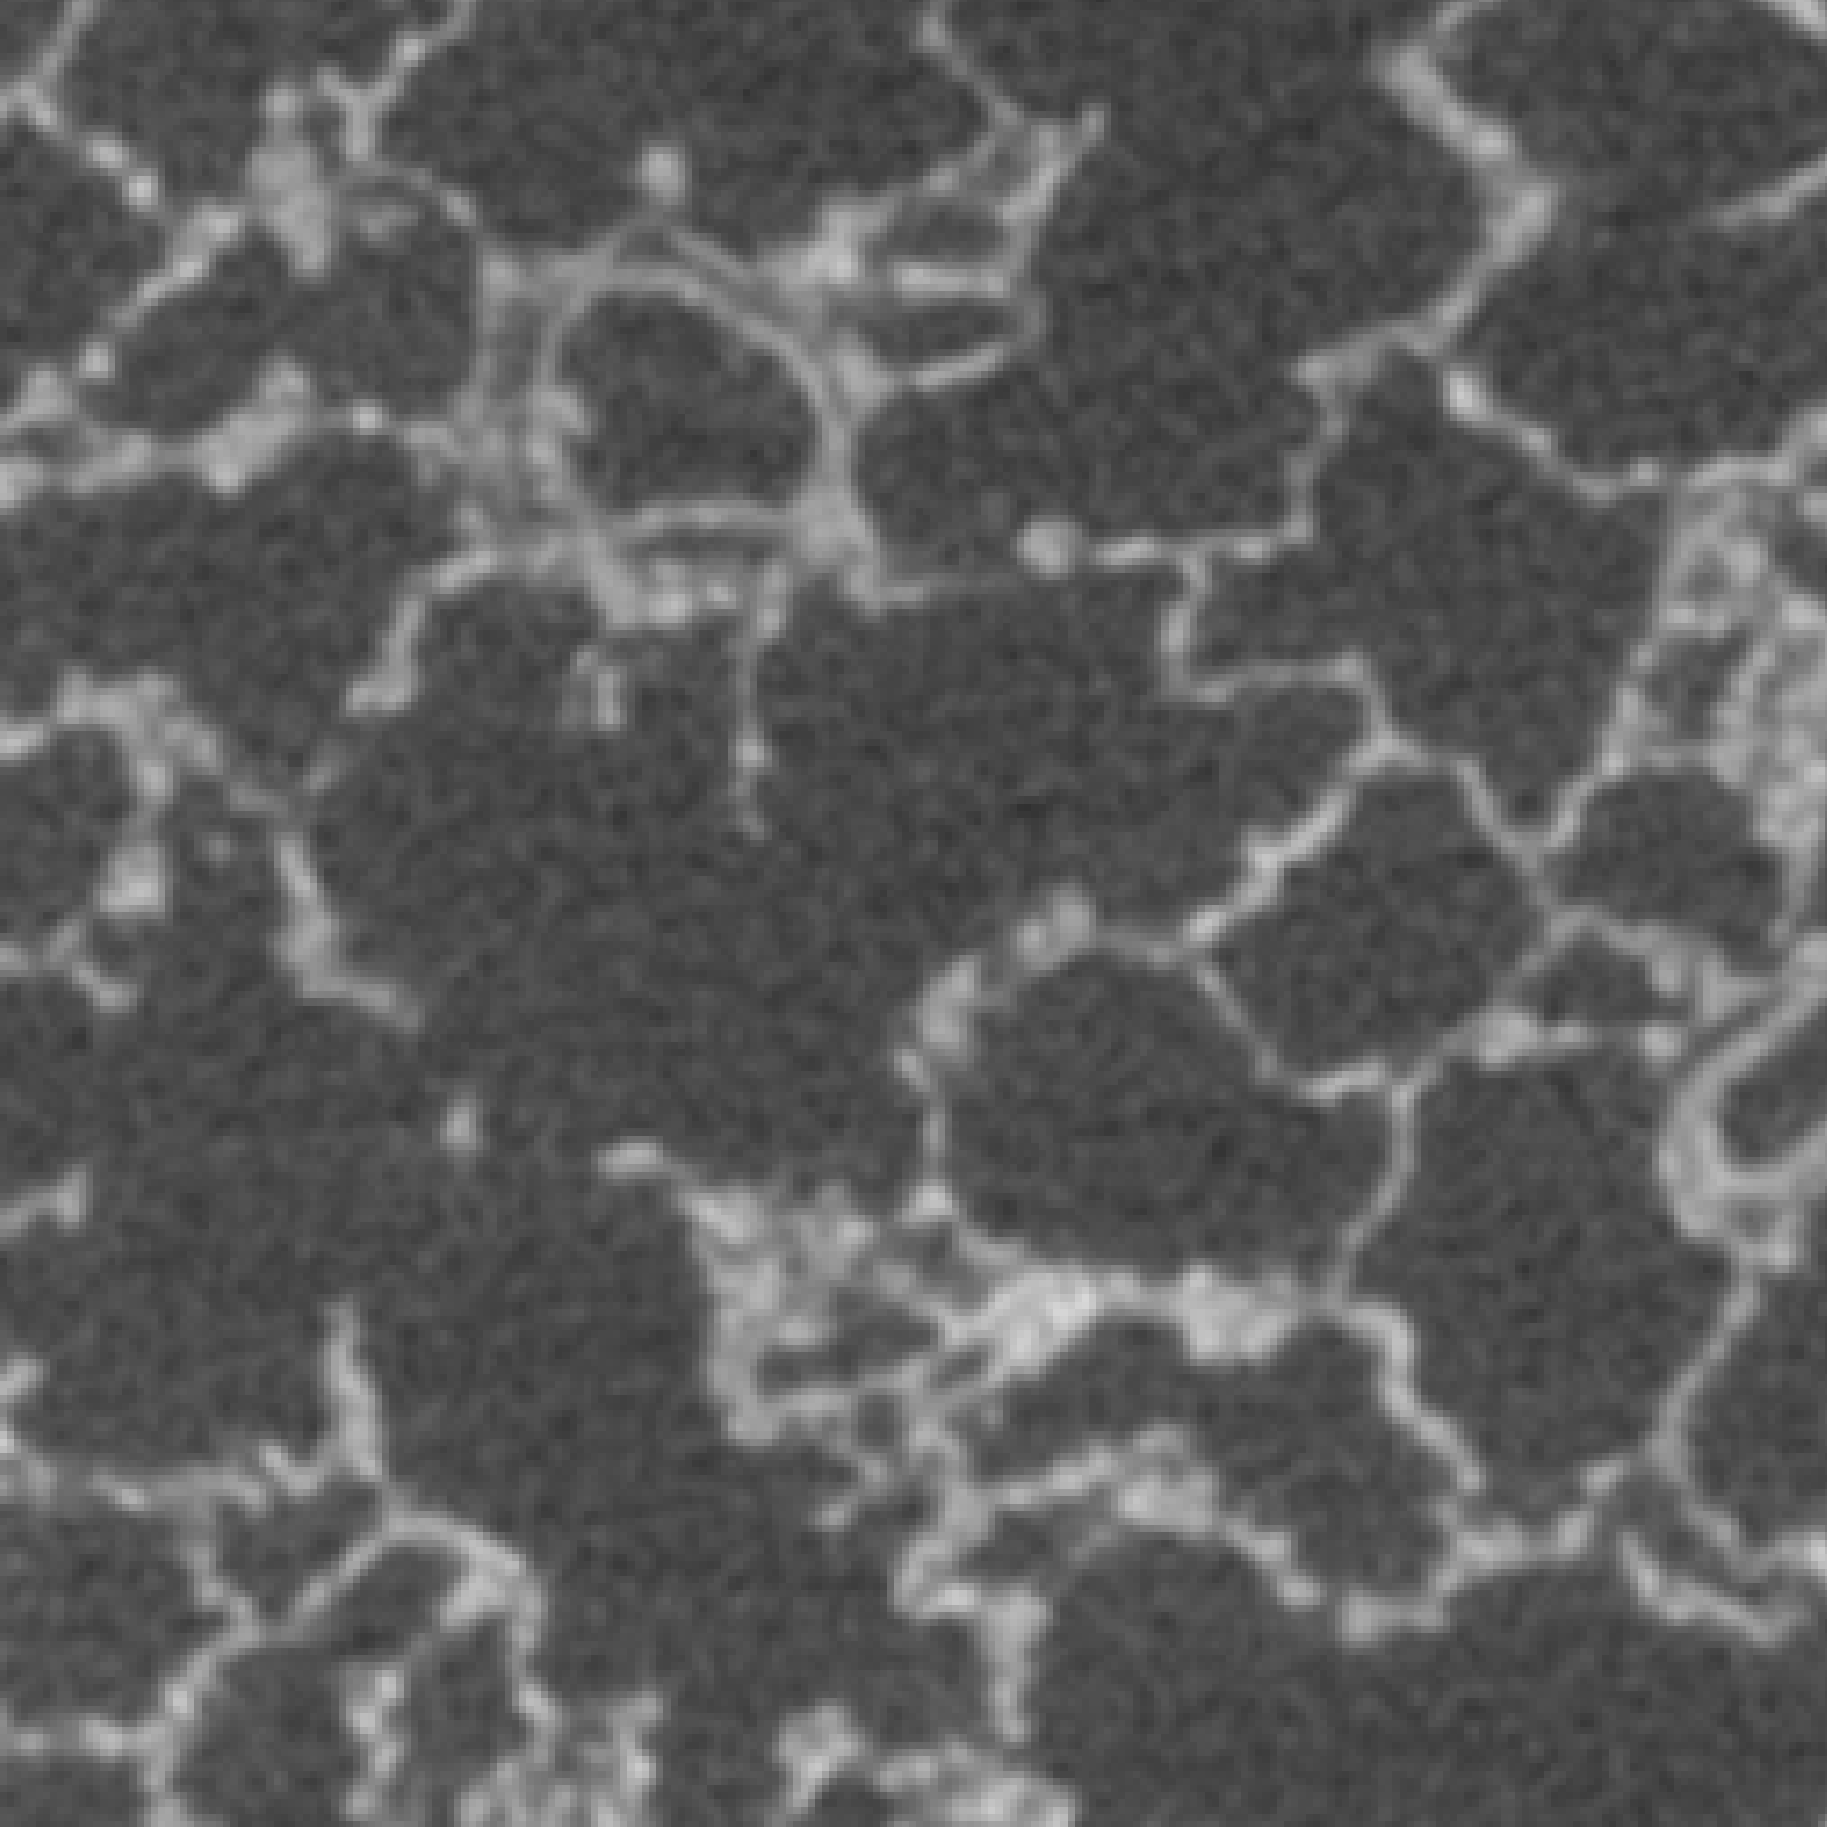
\includegraphics[width=\imsize]{img/Tsuda2008/Tsuda-05d}%
		\label{subfig:tsuda-05d}%
	}%
	\caption[Overview of workflow for the selection of a region of interest]{Overview of workflow for the selection of a \acf{roi}. \subref{subfig:tsuda-05a}: full perspective view of the sample R108C60C-07e with 6 selected orthogonal slices and bounding box of the full sample in orange. The \ac{roi} selected for subfigures \subref{subfig:tsuda-05c} and \subref{subfig:tsuda-05d} is visible in the \textit{top left}. \subref{subfig:tsuda-05b}: close-up of one slice of the full dataset with selected \ac{roi} (side-length of 256 pixels). \subref{subfig:tsuda-05c}: \ac{roi} cut out of the full sample, 6 selected orthogonal slices are shown. \subref{subfig:tsuda-05d}: close-up of the \ac{roi} in subfigure \subref{subfig:tsuda-05b}.}
	\label{fig:tsuda-05}
\end{figure}

\subsection{Segmentation}
As mentioned, the selection of a threshold level has significant affects on segmentation. To demonstrate this, we have segmented a small crop of the original data (\autoref{subfig:tsuda-06a}) with three different threshold values. With a low threshold level, for instance 130, the image would possess too many black voxels and the septa in the lung appear to be too thick (\autoref{subfig:tsuda-06b}). On the other hand, with a higher threshold level, for instance 148, the image would possess too many white voxels and the lung tissue appears to be very thin, with multiple erroneous holes in the septal walls (\autoref{subfig:tsuda-06d}). With an intermediate threshold, for instance 139, the lung structure appears to be reasonable, with a minor amount of holes (\autoref{subfig:tsuda-06c}). The optimal value of the threshold level was iteratively determined by performing a ``readjustment-recalculation'' process to match some of the key morphological parameters in the resulting \threed reconstruction to the gold standard. This is explained below in detail.

\renewcommand{\imsize}{0.333\linewidth}
\setlength{\fboxsep}{-\fboxrule}
\begin{figure}[h]
	\centering
	\subfloat[]{%
		\pgfmathsetlength{\imagewidth}{\imsize}%
		\pgfmathsetlength{\imagescale}{\imagewidth/238}%
		\begin{tikzpicture}[x=\imagescale,y=-\imagescale]
			\def\x{127} % scalebar-x at golden ratio of x=238px
			\def\y{214} % scalebar-y at 90% of height of y=238px
			\node[anchor=north west, inner sep=0pt, outer sep=0pt] at (0,0) {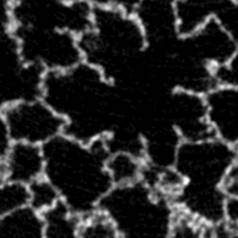
\includegraphics[width=\imagewidth]{img/Tsuda2008/Tsuda-06a.png}};
			% 238px = 0.37888mm > 100px = 159um > 314px = 500um, 63px = 100um
			%\draw[white,|-|,thick] (1,112) -- (239,112) node [sloped,midway,above] {\SI{0.37888}{\milli\meter} (256px)};
			\draw[white,|-|,thick] (\x,\y) -- (\x+31.4,\y) node [right] {\SI{50}{\micro\meter}};
		\end{tikzpicture}%
		\label{subfig:tsuda-06a}%
	}\\
	\subfloat[]{%
		\fbox{%
			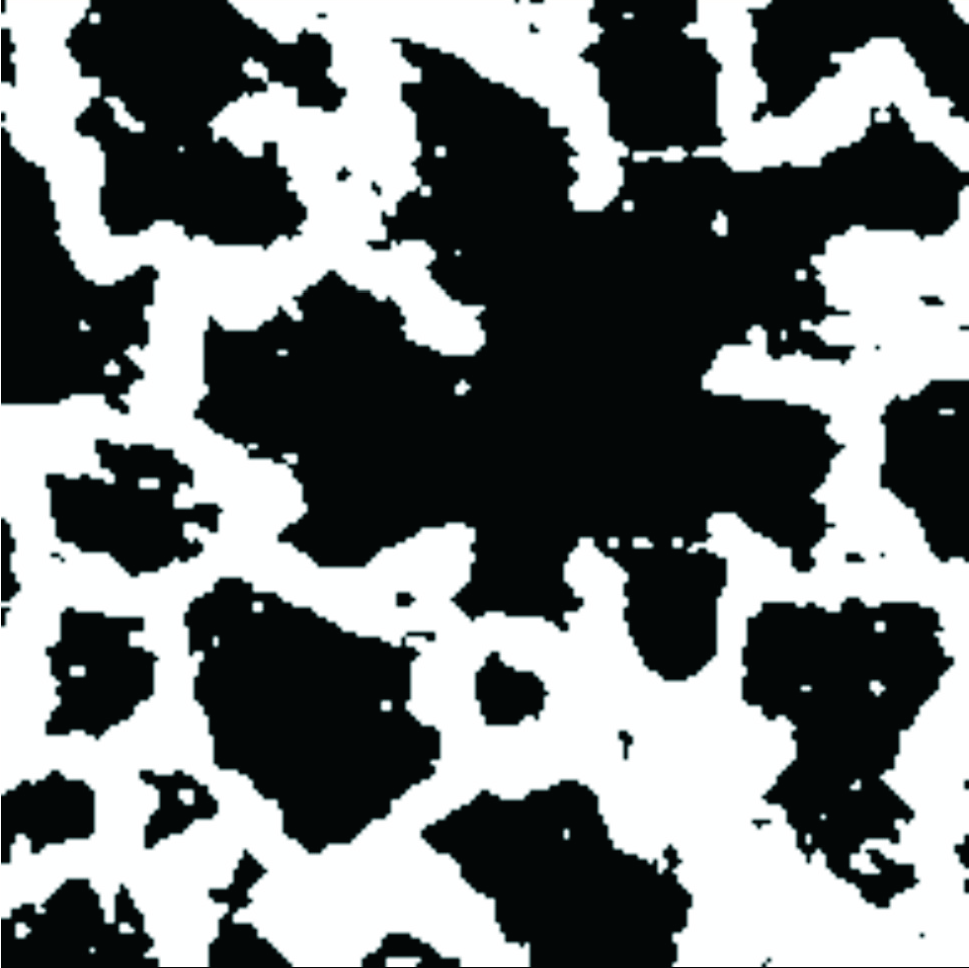
\includegraphics[width=\imsize]{img/Tsuda2008/Tsuda-06b}%
			\label{subfig:tsuda-06b}%
			}%
	}\hfill%
	\subfloat[]{%
		\fbox{%
			
\includegraphics[width=\imsize]{img/Tsuda2008/Tsuda-06c}%
			\label{subfig:tsuda-06c}%
			}%
		}\hfill%
	\subfloat[]{%
		\fbox{%
			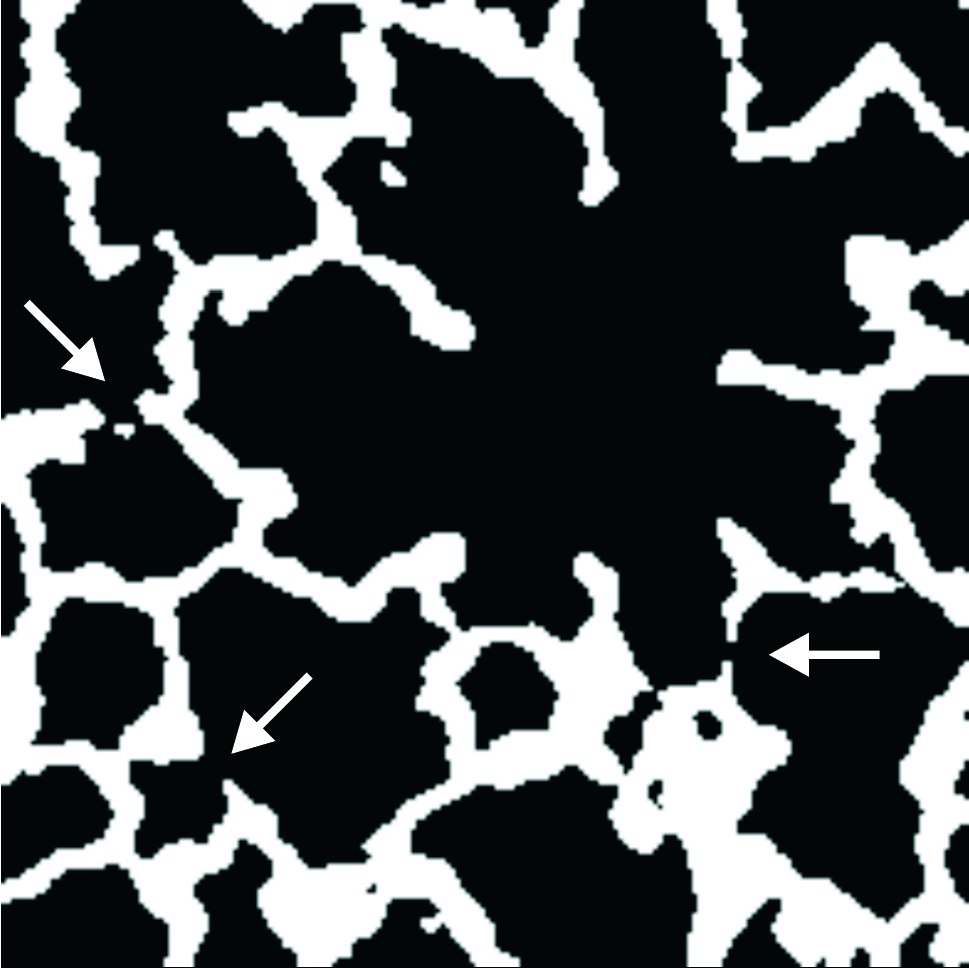
\includegraphics[width=\imsize]{img/Tsuda2008/Tsuda-06d}%
			\label{subfig:tsuda-06d}%
			}%
	}%
	\caption[Thresholding Influence]{\subref{subfig:tsuda-06a}: original slice from raw data. \subref{subfig:tsuda-06b}: thresholded with a value of 130, meaning that all pixels below 130 are set to black, all pixels with a value of 130 or greater are set to white. Resulting alveolar walls are too thick. \subref{subfig:tsuda-06c}: thresholded with a value of 139. Image looks correct. At this threshold the observed thickness of the septa was smaller than \SI{10}{\micro\meter}. In the same animals \cite{Roth2005} the thickness of the septa was determined as they appeared on electron microscopical images. They measured a mean of \SI{8}{\micro\meter}. \subref{subfig:tsuda-06d}: thresholded with a value of 148. Alveolar walls are too thin, and multiple erroneous holes (arrows) appear in the tissue.}
	\label{fig:tsuda-06}
\end{figure}

\subsection{FE \threed reconstruction}
Prior to the \threed reconstruction, the \ was performed to screen small objects with unreasonable size; voxels of those unreasonably small objects were reclassified to match the surrounding voxels. After successful preprocessing, \threed reconstruction was performed using \ac{gbha}. The examples with three different values of threshold level (130, 139, 148), corresponding to those in \autoref{fig:tsuda-06}, are shown in \autoref{fig:tsuda-07}. As is expected, the \threed reconstructed object appears to have thick tissue walls with the lower threshold value of 130, while it appears to be too thin, with many holes with the higher threshold value of 148. With the intermediate threshold value of 139, the structure appears to be reasonable. This will be tested quantitatively next.

\subsection{Validation of Segmentation and Image Processing}
To perform a statistical analysis for the selection of the threshold value, five pieces of parenchymal sample (200$\times$200$\times$180 pixels) were selected. We calculated the V\textsubscript{VS} of each \ac{roi} after the \threed reconstruction, and the average value with \ac{se} was plotted as a function of threshold level (\autoref{fig:VVSplot}). Our calculated value of V\textsubscript{VS} nearly linearly decreased with increasing threshold level and our V\textsubscript{VS} matches the gold standard value of 0.196 at a threshold value of 139. In addition, the values of calculated SE were generally very small, indicating that each sample, although small in size, represented typical parenchymal structure. We determined to use a threshold value of 139 for this tissue sample.

The surface area density of air space (S\textsubscript{VS} [\centimetresquared\per\centimetrecubed]) of each \ac{roi} sample was also calculated and plotted (\autoref{fig:VVSplot}). As we expected, however, S\textsubscript{VS} shows poor match with the reported value of \num[seperr]{904(84)}~(\acs{se}) over almost the entire range of threshold levels tested and especially at the threshold value of 139. The cause of this discrepancy will be discussed in detail in \autoref{sec:discussion}.

\renewcommand{\imsize}{0.333\linewidth}
\begin{figure}[h]
	\centering
	\subfloat[]{%
		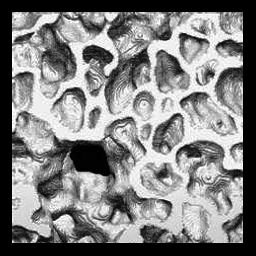
\includegraphics[width=\imsize]{img/Tsuda2008/Tsuda-07a}%
		\label{subfig:tsuda-07a}%
	}%
	\subfloat[]{%
		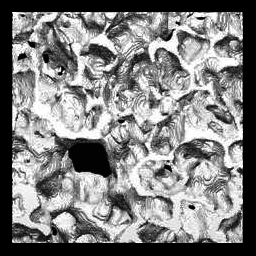
\includegraphics[width=\imsize]{img/Tsuda2008/Tsuda-07b}%
		\label{subfig:tsuda-07b}%
	}%
	\subfloat[]{%
		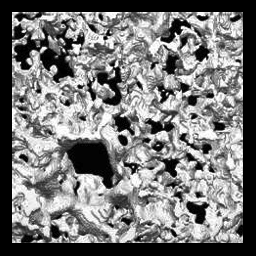
\includegraphics[width=\imsize]{img/Tsuda2008/Tsuda-07c}%
		\label{subfig:tsuda-07c}%
	}\\%
	\subfloat[]{%
		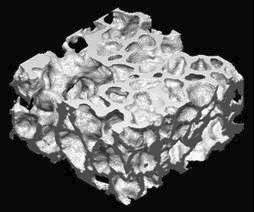
\includegraphics[width=\imsize]{img/Tsuda2008/Tsuda-07d}%
		\label{subfig:tsuda-07d}%
	}%
	\subfloat[]{%
		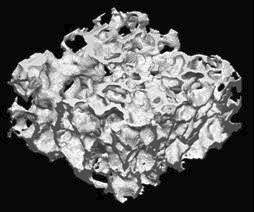
\includegraphics[width=\imsize]{img/Tsuda2008/Tsuda-07e}%
		\label{subfig:tsuda-07e}%
	}%
	\subfloat[]{%
		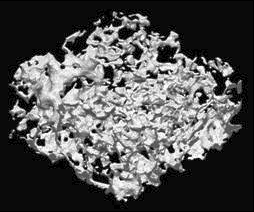
\includegraphics[width=\imsize]{img/Tsuda2008/Tsuda-07f}%
		\label{subfig:tsuda-07f}%
	}\\
	\caption[Three-dimensional reconstruction of tissue]{Three-dimensional reconstruction of tissue. \subref{subfig:tsuda-07a} and \subref{subfig:tsuda-07d}: threshold 130. \subref{subfig:tsuda-07b} and \subref{subfig:tsuda-07e}: threshold 139. \subref{subfig:tsuda-07c} and \subref{subfig:tsuda-07f}: threshold 148.}
	\label{fig:tsuda-07}
\end{figure}

\renewcommand{\imsize}{\linewidth}
\begin{figure}[h]
	\centering
	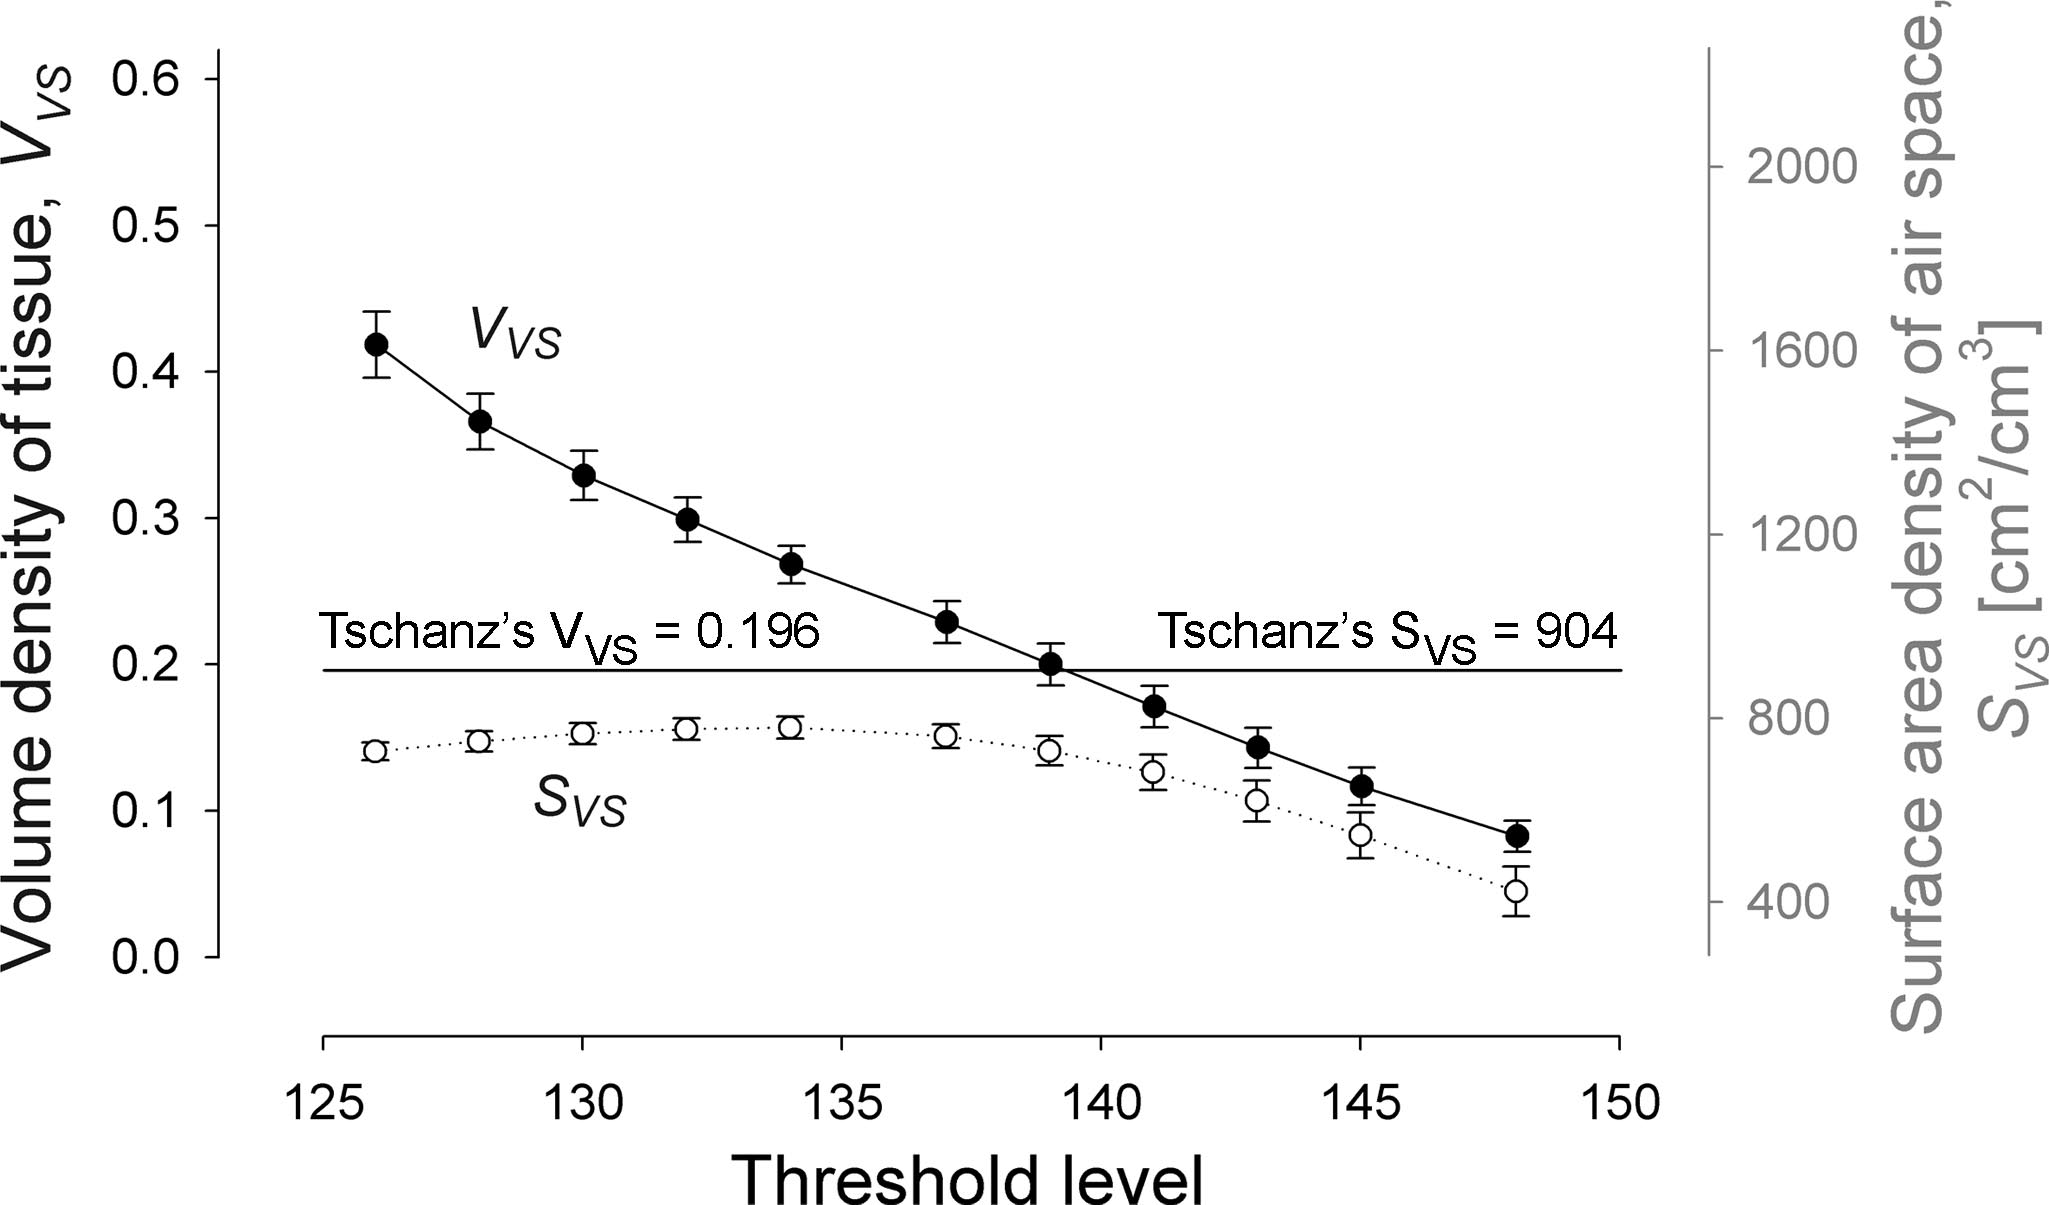
\includegraphics[width=\imsize]{img/Tsuda2008/Tsuda-08}
	\caption[Average volume density of tissue and surface area density of air space]{Average volume density of tissue (V\textsubscript{VS}) and surface area density of air space (S\textsubscript{VS}) of \acp{roi}, plotted as a function of threshold level. Error bars represent standard error. Our V\textsubscript{VS} matches the gold standard value of 0.196 at a threshold value of 139. Bars include the standard error, n=5.}
	\label{fig:VVSplot}
\end{figure}

\subsection{FE \threed Reconstruction of Air Space}
\threed air spaces, separated by tissues, in the \ac{roi} were also constructed (\autoref{fig:tsuda-09}). To demonstrate air space configuration more clearly, a small alveolated air section was isolated from the center of \ac{roi} and was enlarged in an inset of \autoref{fig:tsuda-09}. These \threed air objects packed with several million \threed 8-node \acp{fe} (a mixture of structured and unstructured cubic elements) can be readily used for \ac{fe} calculations, including airflow \ac{cfd}, in the future.

\section{Discussion}\label{sec:discussion}
We described our custom-made \ac{fe} methodology to reconstruct the acinar air space as well as septal tissue of rat lung in three dimensions. Approximately \SI{3}{\milli\meter\cubed} (=3$\times10^9$~\micro\meter$^3$) of fixed lung tissue was scanned with high resolution \ac{srxtm} (voxel size=\SI{1.4}{\micro\meter\cubed}) and a stack of 1024 image slices (1024$\times$1024~pixels) was prepared for \threed rendering. After preprocessing the raw voxel data with a tentative threshold level, \threed \acp{fe} were created overlaying the voxel map using a \ac{gbha}. A proper threshold value for adequate segmentation was iteratively determined to match the calculated volume density of tissue (V\textsubscript{VS}) to the stereological determined value \cite{Tschanz2003}. With the optimized algorithms (a combination of \ac{oca} and \ac{gbha} algorithms), \acsu{cpu} time for one iteration for $\sim$8 million voxels was $\sim$\SI{90}{\min} by a standard \ac{pc}.

\subsection{Historical Perspective}
Acinar structure was traditionally studied using lung cast models \cite{Boyden1971,Haefeli1988,Schreider1981} or serial histological sections (\eg, \cite{Berend1991,Hansen1975,Hansen1975a,Parker1971,Randell1989}). With the former approach, some types of measures are not possible: only the polymer-filled air spaces are available for measurement as the tissue is digested away, and internal data are lost as scanning electron microscopy is limited to the exposed surfaces of the cast. \threed rendering of alveolar geometries from histological sections requires careful, time-consuming alignment and registration of serial \twod sections \cite{Mercer1987,Mercer1987a,Stelter1966}, which generally limits reconstruction to just a few alveoli~\cite{Mercer1987}. An additional drawback is sample destruction and deformation from physical sectioning.

Optical sectioning permits faster, less invasive, more thorough digital analysis and \threed rendering than is possible with physical sectioning. Large upper airways can be analyzed with modern techniques such as magnetic resonance microscopy~\cite{Hoffman1990,Sundaramoorthy1995} or optical coherence tomography~\cite{Hanna2005}; functional imaging of the lung by \ac{ct} and \ac{mri} has recently been summarized by \citet{VanBeek2008}. Laser scanning confocal microscopy provides sufficient resolution to image fine-scale acinar detail, but there have been very few \threed acinar reconstruction studies using this method. \citet{Cookson1993} used serial optical sections acquired by confocal microscopy to produce \threed volume renderings of human alveolar ducts. This approach is restricted in that imaging depth below the tissue surface is limited by light penetration and the working distance of the objective lens~\cite{Bonse1996}. \citet{Cookson1993} warned that caution was necessary in interpreting confocal \threed renderings because the relative contributions of the various factors (refractive index changes, tissue density changes, resorption) causing depth-dependent loss of resolution and/or intensity were difficult to measure and correct. Multiphoton microscopy improves imaging depth, but the imaging depth is still restricted to $\sim$\SI{100}{\micro\meter} into the lung \cite{Pena2007}. For comparison, human alveolar ducts range from 270 to \SI{600}{\micro\meter} in diameter \cite{Whimster1970}. Thus sample size constraints limit confocal analysis to just a small portion of the acinus, restricting its usefulness in studies of flow and aerosol particle deposition. In the early 1990s, new imaging techniques, such as \ac{ct} \cite{Brown1991,Mcnamara1992}, permitted measurement and reconstruction of the \threed structure of the bronchial tree and small airways \cite{Aykac2003,Higgins1998,Park1998,Reinhardt1997,Sauret2002,Sera2003,Wood1995,Wood1995a}. Successful visualization of the acinar region, though, was limited by the spatial resolution of standard \ac{uct}. In the past few years, however, \ac{uct}-based \threed reconstruction and morphometric analysis of the alveolar region has become possible \cite{Langheinrich2004,Litzlbauer2006,Watz2005}, facilitated by the advent of \ac{srct}. \ac{srct} is to be distinguished from \ac{srxtm} \cite{Schittny2008,Stampanoni2002,Stampanoni2007}. While during \ac{srct} the X-rays are directly recorded after transmitting the sample, during \ac{srxtm} the transmitted images are first recorded on a scintillator and magnified 5--20 times by a light microscope before recording.

\subsection{srxtm}
\ac{sr} is an electromagnetic wave emitted from electrons traveling near the speed of light when their path is bent by a magnetic field \cite{Iida2003}. A synchrotron facility is an excellent source of the most useful electromagnetic waves to explore materials and biological systems: X-ray ultraviolet and infrared light. Here we limit our discussion particularly to the application of \ac{sr} for X-ray tomographic microscopy (\autoref{fig:imaging setup}) highlighting the following superb features.

\renewcommand{\imsize}{0.5\linewidth}
\begin{figure}[h]
	\centering
	\subfloat[]{%
		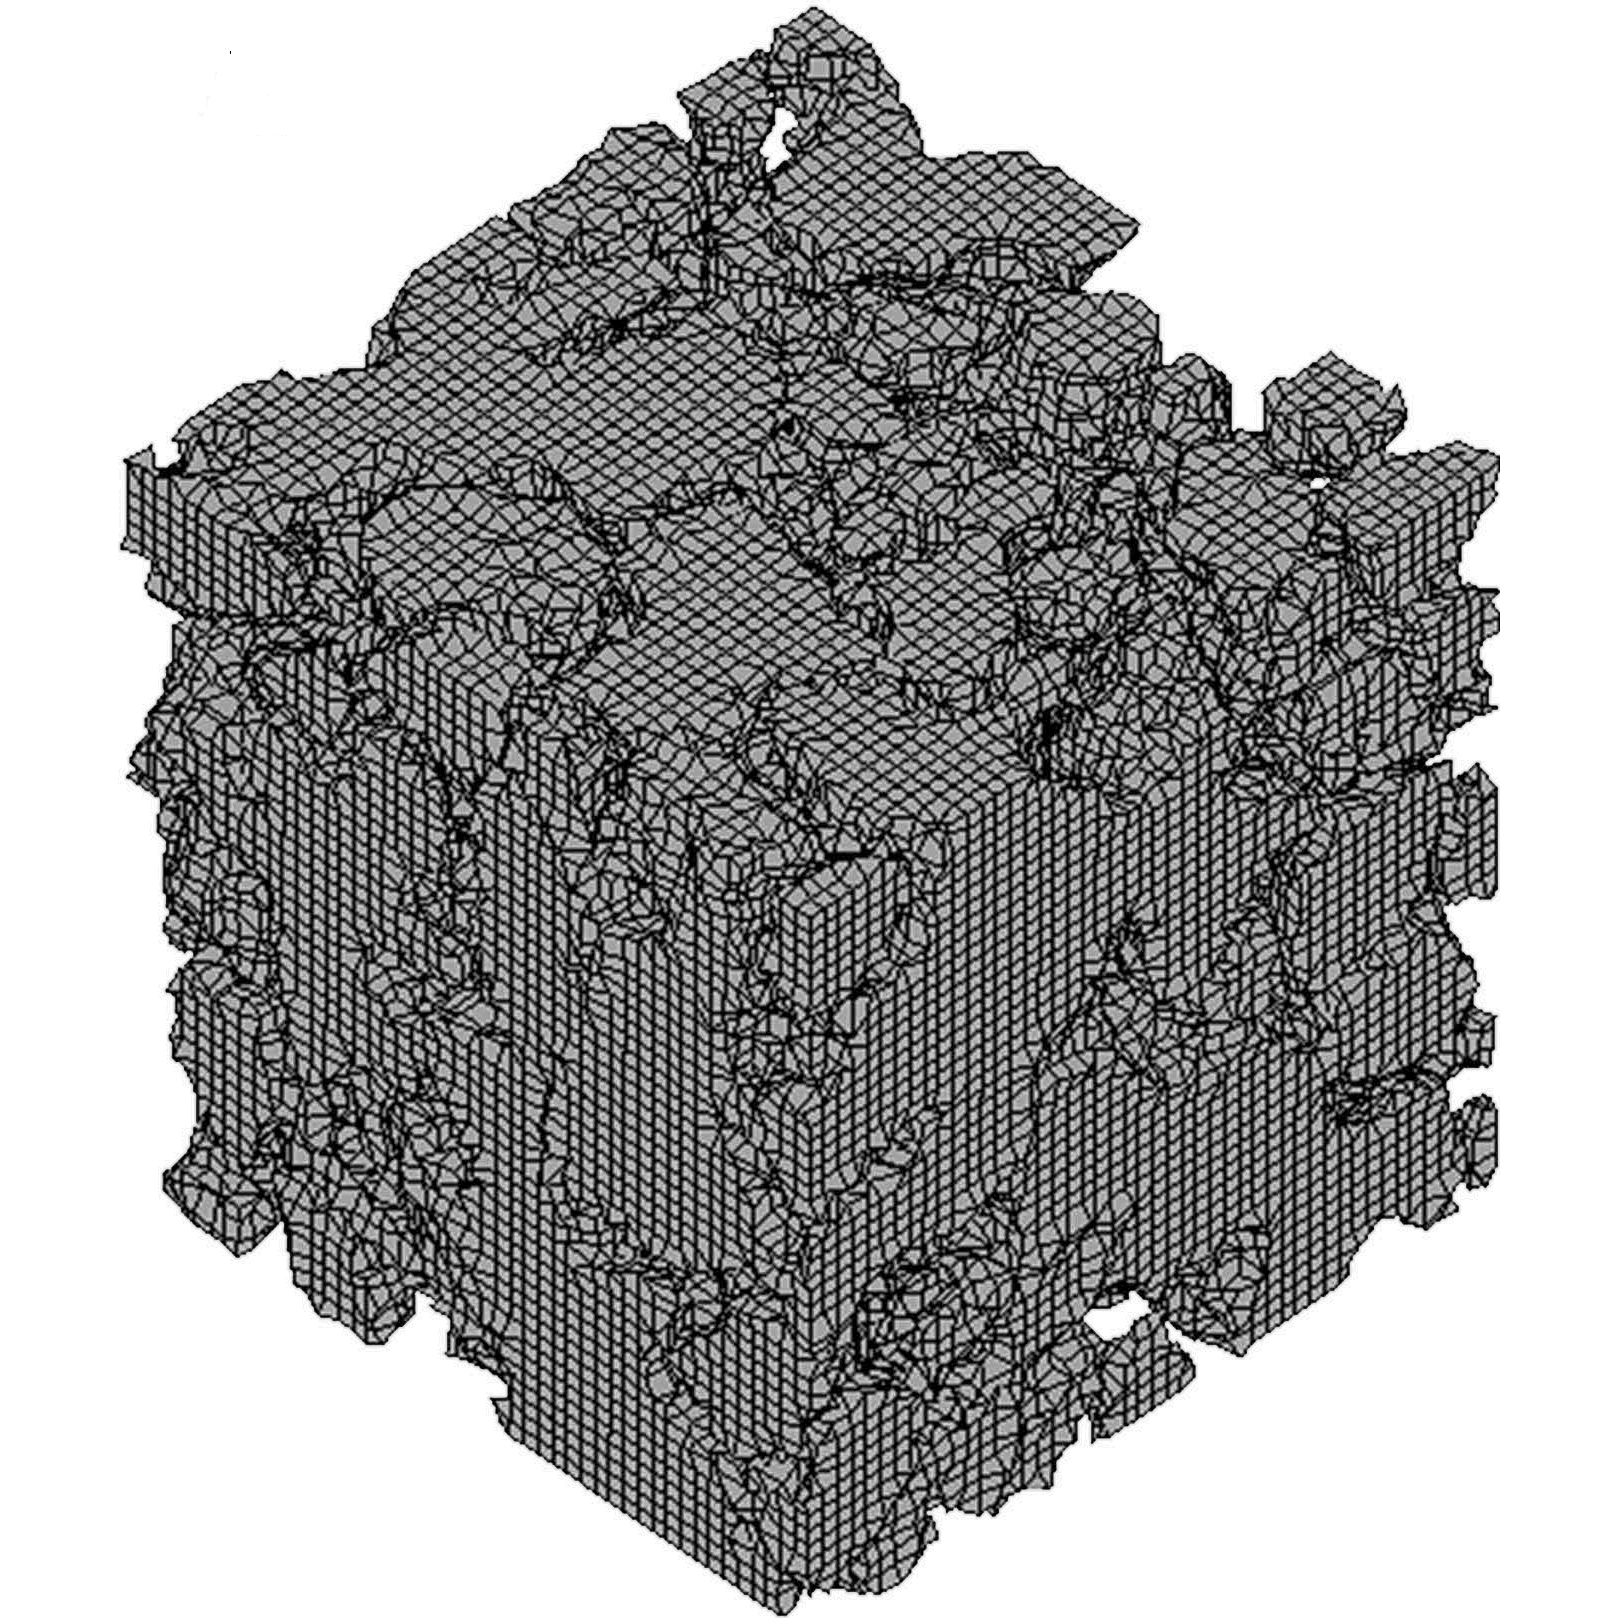
\includegraphics[width=\imsize]{img/Tsuda2008/Tsuda-09a}%
		\label{subfig:tsuda-09a}%
	}\hfill%
	\subfloat[]{%
		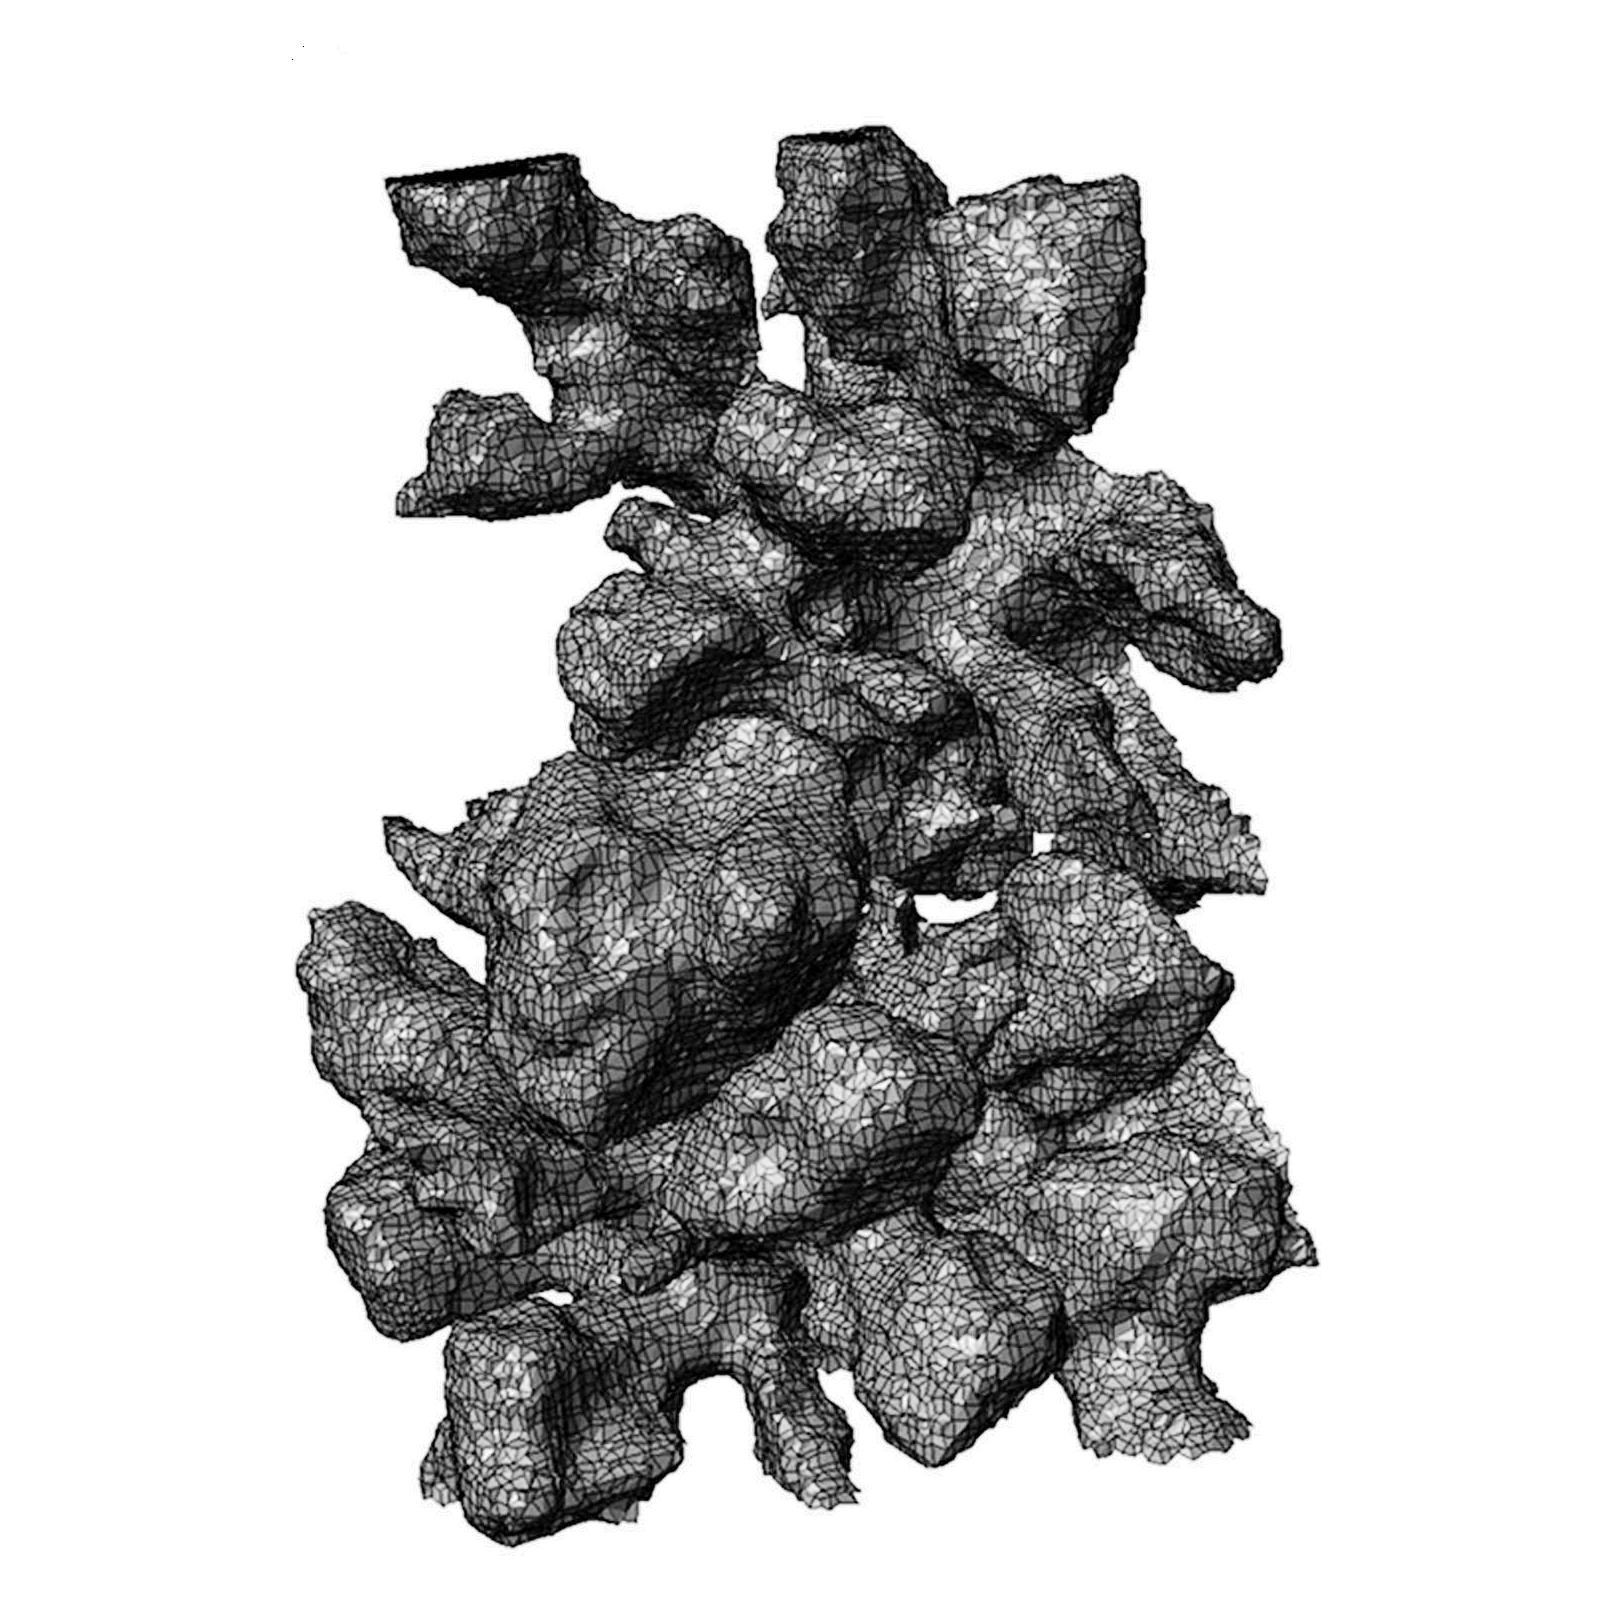
\includegraphics[width=\imsize]{img/Tsuda2008/Tsuda-09b}%
		\label{subfig:tsuda-09b}%
	}%
	\caption[Three-dimensional reconstruction of air spaces]{\subref{subfig:tsuda-09a}: reconstruction of \threed air spaces separated by tissues from \ac{roi}. \subref{subfig:tsuda-09b}: enlargement of a small alveolated air section isolated from the center of the \ac{roi}.}
	\label{fig:tsuda-09}
\end{figure}

\subsubsection{High power and high brilliance}
\ac{sr} is extremely powerful but even more important is that this radiation is emitted by a small source area and that this emission occurs within a narrow angular cone. Bending magnets or sophisticated insertion devices (called undulators or wigglers) produces therefore a high brilliant radiation that is several orders of magnitude more bright than conventional X-ray tubes (\autoref{fig:imaging setup}). This makes the usage of monochromators\graffito{A monochromator is a device in X-ray optics that is used to select a defined wavelength of the radiation for further use in a dedicated instrument or beamline.} particularly interesting since an extremely intense photon flux at a selected energy (or wavelength) can easily be extracted from the white beam emitted by the source (\autoref{fig:imaging setup}). The X-ray energy can be adjusted ``ad hoc'' to the sample, according to its absorption properties. The monochromaticity of the beam is an important feature of \ac{sr} application, critical for tomography applications since it automatically eliminates beam hardening artifacts from the tomographic reconstruction.

The high collimation of the \ac{sr} produces ``de facto'' a parallel beam at the sample location: the resulting negligible geometrical blur makes it possible to obtain images with high spatial resolution and a high \ac{snr}. Since, for a given \ac{snr} and a given contrast, the necessary photon flux scales with the fourth power of the spatial resolution \cite{Bonse1996} it is obvious that \ac{sr}-based tomography is perfectly suited for investigations with spatial resolution in the micrometer or even submicrometer range. Nowadays, X-ray tomographic microscopy endstations installed at third generation synchrotron facilities like \ac{tomcat}~\cite{Stampanoni2007} routinely reach resolution $\sim$\SI{1}{\micro\meter} within scan times of a few minutes.

Synchrotron radiation-based \ac{ct} overcomes the critical technical issue (resolution) that has prevented fine-scale structural analysis of the acinus by tabletop X-ray \ac{uct}. The brilliant, highly collimated beam provides a nearly ideal X-ray source for \ac{uct}~\cite{Jorgensen1998}, producing greater spatial resolution. This allows high-resolution imaging of unprocessed lung tissue \cite{Bayat2006,Jheon2006,Monfraix2005,Sera2007,Sera2005} and ultra high resolution (from $<$1 to \SI{15}{\micro\meter}, with tissue thicknesses of $\geq$\SI{1500}{\micro\meter}) visualization and \threed reconstruction of small airways and alveoli in processed tissue \cite{Ikura2004,Schittny2008}.

\subsection{Segmentation/Threshold}
Careful determination of the proper threshold level is essential for accurate \threed rendering and for the first step of \ac{fe}-mesh generation. If the level is too low, the fraction of air would become unrealistically small relative to tissue resulting in thicker septa. If the level is too high, on the other hand, the fraction of air becomes unrealistically large relative to tissue; thinner tissue would result in artificial holes in the septal walls or even too many unconnected tissue pieces in the sample. This would have a direct impact on the skeletonization process (which is not dealt with in this paper), as well as the subsequent \ac{fe} analyses, such as airflow simulations. Our \ac{oca} is designed to minimize this problem.

A unique aspect of our work is that segmentation was done iteratively by searching for the optimal threshold value (\autoref{fig:workflow}). In every iteration, the key morphological parameter (discussed below in detail) was calculated and compared with the gold standard; the iteration was continued until the calculated value matched the gold standard. This gold standard was previously determined in the tissue sample from exactly the same animal~\cite{Tschanz2003}. Because our main aim in this work was to develop \ac{fe} methodology, this selection of tissue sample, whose morphology has been thoroughly analyzed, is very well suited for this project.

The key morphological parameter we tried to match was the volume density of tissue (V\textsubscript{VS}). The V\textsubscript{VS} is an easy to calculate parameter (\ie, the sum of \ac{fe} volume belonging to tissue divided by the sum of all \ac{fe} volume) and is relatively insensitive to the resolution of the measurement technique. The calculated V\textsubscript{VS} decreases almost linearly with an increase in the threshold level (\ie, a fraction of air volume relative to tissue volume) around the gold standard value (V\textsubscript{VS}=0.196 in our case, see \autoref{fig:VVSplot}). At the threshold value of 139, the calculated V\textsubscript{VS} was within \SI{2}{\percent} difference of the gold standard.

\renewcommand{\imsize}{\linewidth}
\begin{figure}[ht]
	\centering
	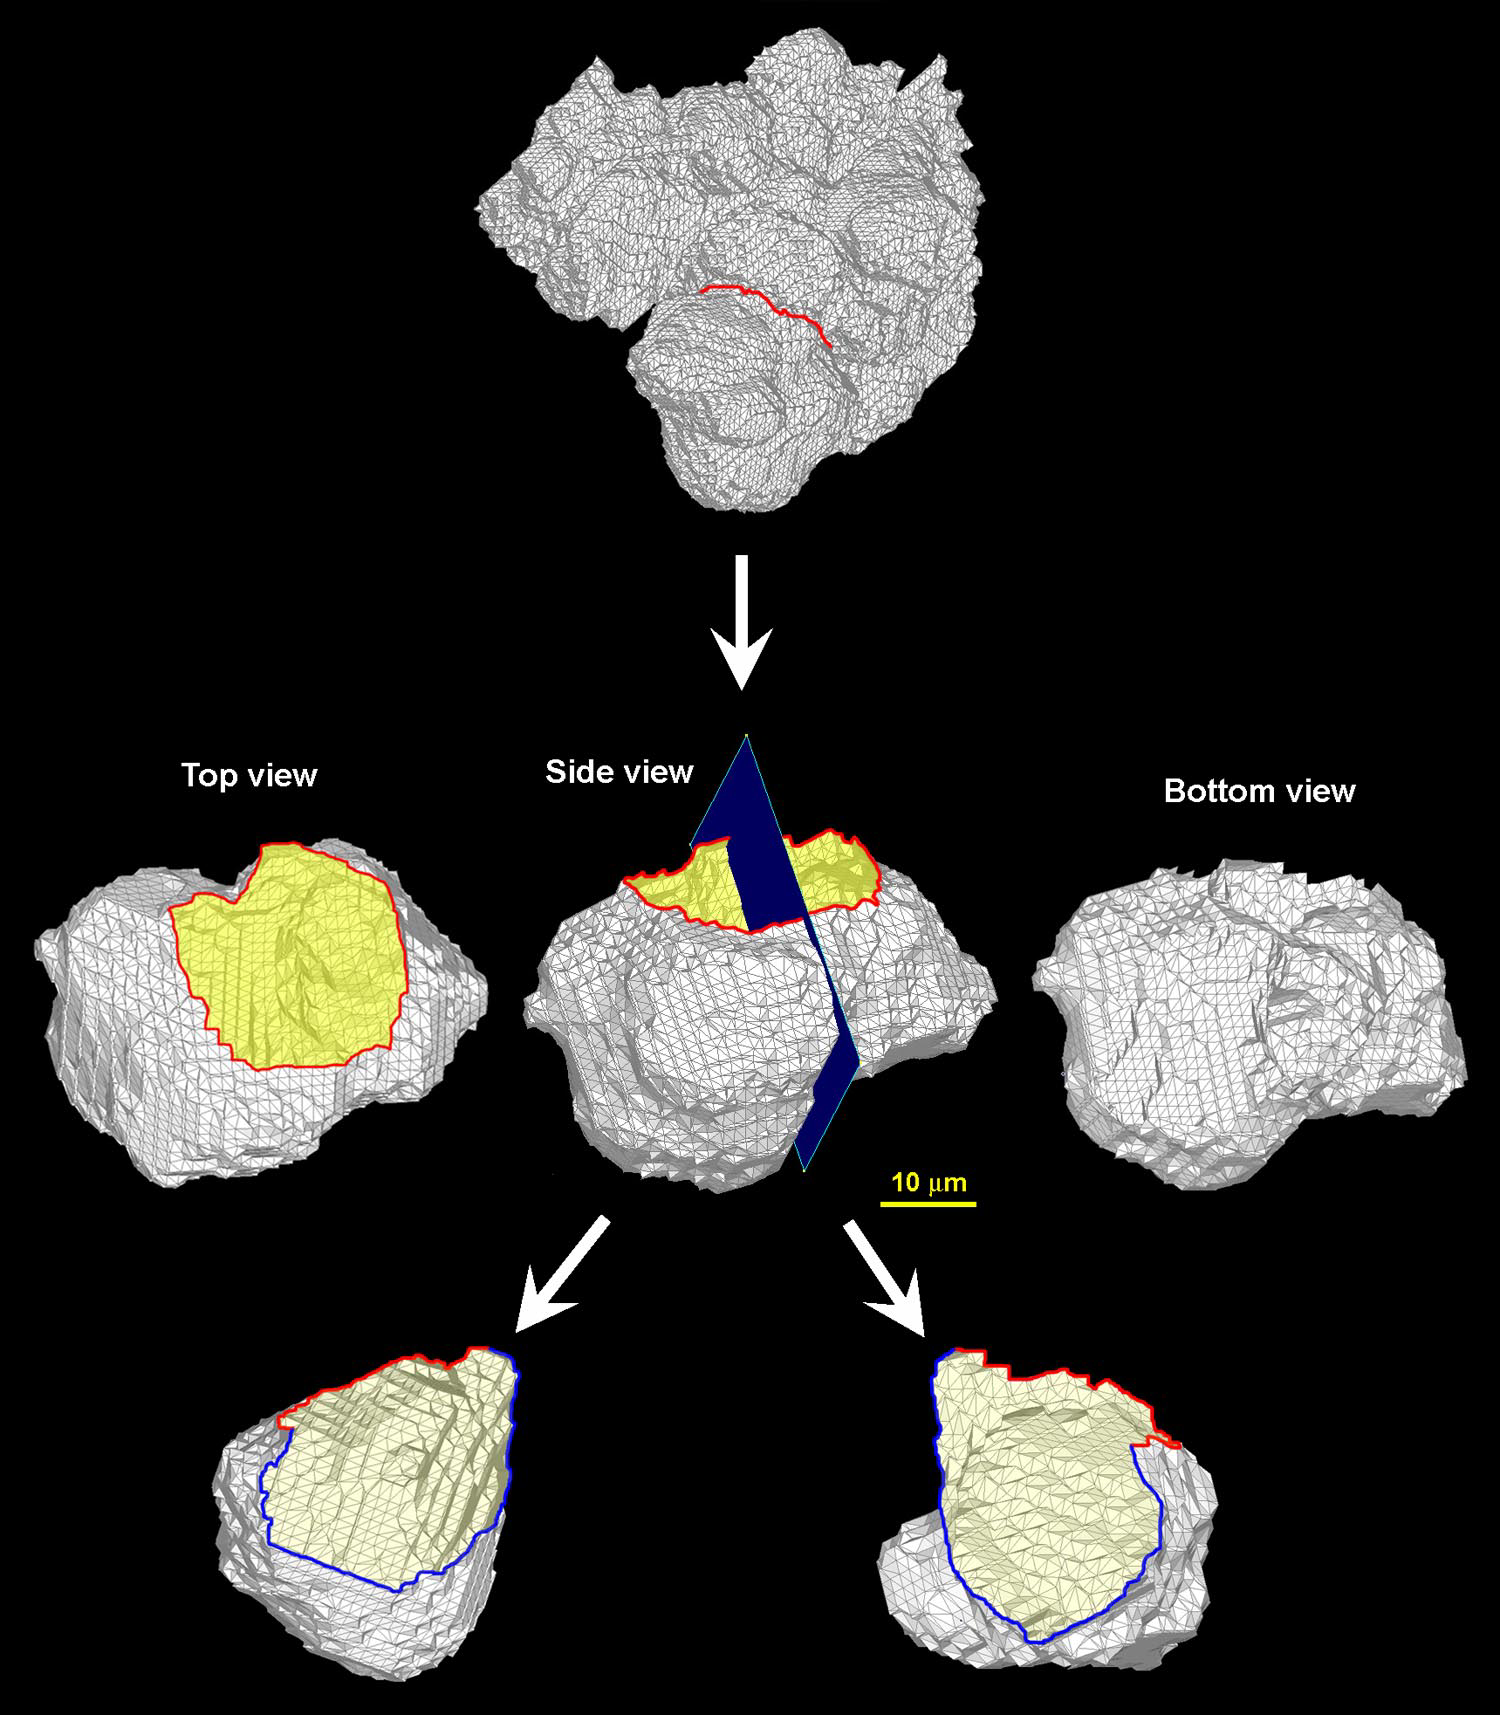
\includegraphics[width=\imsize]{img/Tsuda2008/Tsuda-10}
	\caption[Three-dimensional FE shell model of a partial acinus]{Three-dimensional \ac{fe} shell model of acinus viewed from different angles. Top: \ac{roi}. Middle: top view (\textit{left}); side view (\textit{middle}); bottom view (\textit{right}). Bottom: alveolar inside views.}
	\label{fig:alveolus}
\end{figure}

We also calculated surface area density of air space (S\textsubscript{VS} [\centimetresquared\per\centimetrecubed]) and compared it with the value reported by \cite{Tschanz2003}. However, our calculated values were always lower than the reported value (S\textsubscript{VS}=904 [\centimetresquared\per\centimetrecubed]). This is because although the volume is relatively insensitive to the resolution of the measurement technique, the air-tissue boundary (surface area) is highly sensitive to how it is measured. S\textsubscript{VS} reported in \citet{Tschanz2003} was measured at a $\times$10 secondary magnification after recording the electron microscopical images at a primary magnification of $\times$1200 on a \SI{35}{\milli\meter} film (theoretical resolution of $\sim$\SI{70}{\nano\meter}), while the resolution of our \threed reconstruction is \SI{1.4}{\micro\meter}. The extent of surface complexity is recognized differently, depending on the resolution of the measuring instrument; the finer the resolution of the sample and the instrument, the more surface detail can be detected. This is similar to the problem when one measures the length of the British coastline with different yardsticks~\cite{Mandelbrot1967}.

\subsection{\twod vs. \threed}
Morphological analyses in \threed are qualitatively different from stereology, which is an analysis made in \twod sections to infer \threed structure and morphometry. Apart from the most common measures of geometric/topological properties, such as the volume density, the area density, and the length density, stereological analysis is generally limited. For example, number density cannot be estimated stereologically using single sections without a significant number of a priori assumptions about the shape of the objects, including the question of whether the objects are convex and whether they are simply connected. These significant restrictions in the stereological analysis are due to the fact that it is based on the following two fundamental assumptions: 
\begin{enumerate}
	\item the structure is homogeneously distributed (\ie, spatially invariant) and 
	\item isotropically distributed (\ie, rotation invariant) in the tissue sample (J. P. Butler, personal communication). 
\end{enumerate}
The \threed analysis relaxes these restrictions either by going to full unrestricted \threed (\ac{uct}, \ac{mri}, \ac{srxtm}, etc.) or using two consecutive sections (disector) for the counting of numbers~\cite{Hyde2007}.

In addition to these fundamental differences, \threed analyses have numerous advantages over traditional stereology. The most obvious advantage is the flexibility of the analysis. It is often difficult to properly select a \ac{roi} because the exact location of the target region cannot be identified beforehand and in the traditional approach, one has only one opportunity to section the tissue sample. In the case of \threed reconstruction analysis, on the other hand, the selection of the \ac{roi} can be repeated as many times as required and the selection can be iteratively improved until the target \ac{roi} is obtained. Once the \ac{roi} is selected in \threed (\autoref{fig:alveolus}, \textit{top}), the target region (\eg, an alveolus) can be viewed from any arbitrary angle (see \autoref{fig:alveolus}, \textit{middle}), including from behind the object (\autoref{fig:alveolus}, \textit{middle right}), something not easily achievable otherwise. The \threed object can be cut into half (\autoref{fig:alveolus}, \textit{bottom}) and also be sliced to make \twod sections in any orientation with any slab thickness (data not shown) and there is no limitation in repeating the sectioning process. Furthermore, since the \ac{roi} can be viewed in any chosen angle and an internal view is possible, it is possible to fly through the structure to gain an internal view of the conduit once the \threed reconstructed structure is electronically available.

\subsection{FE \threed Rendering}
It is important to make a clear distinction between our \ac{fe} \threed rendering approach and the traditional surface triangulation approach that is most common in medical imaging software. The triangulation approach is mainly used for surface visualization; this uses a variety of filtering methods and surface smoothing techniques, but does not involve real volume like with our \ac{fe} \threed rendering method. If the volume compartment of either air or tissue is needed for subsequent analysis, such as for a calculation of fluid flow in acinar air space, a traditional surface triangulation approach does not provide a readily usable \threed structure; a volume bounded by the visualized surface needs to be further elementalized. Since we are in possession of a closed workflow for the further processing of the meshed surfaces (\ie, there is a single process from mesh generation through to visualization), intermediate conversions of the dataset into other formats are not required. This eliminates overhead and speeds the overall process. The \ac{fe} mesh of the data makes it possible to use it for volume rendering, further processing (with the use of quasi-standard \acs{stl} file format\graffito{An \acs{stl} file describes a raw unstructured triangulated surface by the unit normal and vertices of the triangles using a \threed Cartesian coordinate system.}), and direct import into the software used for \ac{cfd} calculations and evaluation of morphological factors. Since we also obtain a mesh inside the structure, we lay the groundwork for the skeletonization (extraction of the mean middle line) of the terminal airways and the determination of the entrance ring of a single alveolus.

The main aim of this project is a direct elementalization of air (or tissue) space using \ac{fe} technique. By isolating air (or tissue) from the rest (tissue or air, respectively), the interface of these two volume components, \ie, an air-tissue barrier, is automatically identified. For this isolation, we adapted the \ac{gbha} proposed by \citet{Schneiders1996}. First, an \ac{fe} mesh was overlaid on the voxel map. Basically, a relation of one \ac{fe} to one voxel could be used, but one practical problem may arise. That is, if the number of voxels in the original data is too large (i.e., in an order of billion in the case of our raw data) for a common \ac{pc} to handle easily, we may need to reduce the number ratio between \ac{fe} and voxel. The important points to achieve are, generally, 
\begin{enumerate}
	\item to reduce the number of \acp{fe} to a reasonable number but
	\item to still produce a smooth surface boundary.
\end{enumerate}
We use hexahedral \ac{fe} for this. An air-tissue interface was smoothed by adjusting the locations of \ac{fe} nodal points near the interface based on their original grayscale pixel intensity values. The distortions of \ac{fe} elements, if this happened as a result of the initial nodal relocation, were corrected and refined (see \autoref{sec:methods} for details). The resulting \threed \ac{fe} mesh (\eg, Figures~\ref{fig:tsuda-09} and \ref{fig:alveolus}) demonstrates reasonable acinar volume rendering.

Finally, for the type of image analysis discussed in this paper, the need for massive computation for \threed rendering as well as subsequent \ac{fe} computational analyses is unavoidable. In this regard, improving our computational capability, particularly by using parallel and grid computing algorithms, would be required in the near future.

\section{Acknowledgments}
We thank F. Marone and C. Hintermüller (Swiss Light Source, Paul Scherrer Institute) for expert help at the Beamline; B.\ de Breuyin, K.\ Sala-Szymanska, and B.\ Haenni for the embedding and preparation of the samples; C.\ Lehmann for the tricky shaping of the samples on the lathe; and D.\ Petrovic for preparing \autoref{fig:alveolus}. We also thank J.\ P.\ Butler and S.\ Tschanz for useful discussion on the subject of stereology.

This work was supported by National Heart, Lung, and Blood Institute Grants HL-054885, HL-070542, and HL-074022, Serbian Ministry of Science, OI144028, TR12007, and Swiss National Science Foundation Grant 3100A0-109874/1.
%\bibliographystyle{plainnat}
%\label{app:bibliography} 
%\bibliography{../Bibliography,../../references,../Tsuda2008references}
% !TEX root = ../Thesis.tex
\acresetall
\myChapter[Radiation dose optimized expansion of the field of view]{Radiation dose optimized lateral expansion of the field of view in synchrotron radiation x-ray tomographic microscopy}\label{ch:haberthuer2010}

David Haberthür\footremember{ana3}{Institute of Anatomy, University of Bern, Bern, Switzerland}\textsuperscript{,}\footnote{\href{mailto:haberthuer@ana.unibe.ch}{haberthuer@ana.unibe.ch}}\\
Christoph Hintermüller\footremember{psi3}{Swiss Light Source, Paul Scherrer Institut, Switzerland}\textsuperscript{,}\footremember{eth3}{Institute for Biomedical Engineering, University and ETH Zürich, Switzerland}\\
Federica Marone\footrecall{psi3}\\
Johannes C. Schittny\footrecall{ana3}\\
Marco Stampanoni\footrecall{psi3}\textsuperscript{,}\footrecall{eth3}\textsuperscript{,}\footnote{\href{mailto:marco.stampanoni@psi.ch}{marco.stampanoni@psi.ch}}\\\\
First published in: Journal of Synchrotron Radiation, 2010\\
\href{http://journals.iucr.org/s/}{doi:10.1107/S101010}
\vspace{52mm}

\section{Abstract}
Volumetric data at micrometer level resolution can be acquired within a few minutes using synchrotron radiation based tomographic microscopy. The field of view along the rotation axis of the sample can easily be increased by stacking several tomograms, allowing  the investigation of long and thin objects at high resolution. On the contrary, an extension of the field of view in the perpendicular direction is non trivial. This paper presents an acquisition protocol which increases the field of view of the tomographic dataset perpendicular to its rotation axis. The acquisition protocol can be tuned as a function of the reconstruction quality and scanning time. Since the scanning time is proportional to the radiation dose imparted to the sample, this method can be used to increase the field of view of tomographic microscopy instruments while optimizing the radiation dose for radiation sensitive samples and keeping the quality of the tomographic dataset on the required level. This approach, dubbed wide field synchrotron radiation tomographic microscopy, can increase the lateral field of view up to five times. The method has been successfully applied for the three-dimensional imaging of entire rat lung acini with a diameter of \SI{4.1}{\milli\meter} at a voxel size of \SI{1.48}{\micro\meter}.

\section{Introduction}
The functional respiratory lung unit---the so-called acinus---is defined as the complex of alveolated airways distal of a last purely conducting airway, the terminal bronchiole~\cite{Rodriguez1987}. The total of all acini forms the lung parenchyma, the area where the pulmonary gas-exchange takes place. While the structural development of the gas-exchange region including the alveolar septa is quite well characterized~\cite{Schittny2007a,Schittny2008,Mund2008}, the development of the three-dimensional structure of its functional unit---of the acini---was not much studied due to the lack of suitable methods.

It is our goal to study the branching pattern of the acinar airways as well as the airflow within it. Tomographic methods, in particular synchrotron radiation based tomographic microscopy can access this kind of information nondestructively and noninvasively.

In order to visualize the thin sheets of tissue (alveolar septa) forming the gas-exchanging alveoli, a resolution in the order of one micron is required. An entire acinus is usually larger than the field of view of the tomographic microscope~\cite{Rodriguez1987,Weibel2009}, being the latest limited by the chosen optical configuration. Usually, a large field of view resulting in a large sample volume can only be acquired with low magnification and vice-versa. Lab-based \acf{uct} stations could potentially be used to study acini, but the resolution of such systems is too low to resolve all alveolar septa. Even if \ac{uct} stations are catching up, synchrotron radiation based tomographic microscopy beamlines provide the necessary high resolution combined with unmatched image quality.

Up to now, the price to pay for this high resolution was a limited field of view. For instance at the beamline for \acf{tomcat} \cite{Stampanoni2007} at the \acl{sls}, Paul Scherrer Institute, Villigen, Switzerland, the field of view at a 10$\times$ magnification (\SI{0.74}{\micro\meter} voxel size) is limited to 1.52$\times$\SI{1.52}{\milli\meter}, insufficient for the imaging of an entire acini at high resolution.

Increasing the field of view perpendicular to the rotation axis of the sample cannot easily be achieved by placing tomographic datasets next to each other. It is instead necessary to merge several projections overlapping the desired field of view prior to tomographic reconstruction. Obviously, to satisfy the sampling theorem, increasing the field of view also requires to acquire more projections, finally resulting in an increased acquisition time.

We developed such a method to merge several independently acquired sets of projections to increase the field of view of the resulting tomographic dataset. In addition, by optimization of the number of recorded projections, we established different scanning protocols with a user-defined balance between acquisition time and image quality.

Because the total acquisition time is directly linked to the radiation imparted to the sample, it is obvious that such protocols also affect radiation damage and constitute an important optimization tool for radiation sensitive experiments.

\section{Materials and Methods}\label{sec:materials and methods}
\subsection{Sample Preparation}
Rat lung samples, prepared according to \citet{Tschanz2002} and \citet{Luyet2002} were used as test objects. Briefly, lungs of Sprague-Dawley rats were filled with \SI{2.5}{\percent} glutaraldehyde (\cf{CH2(CH2CHO)2}) in \SI{0.03}{\Molar} potassium-phosphate buffer (pH 7.4) by instillation via tracheotomy at a constant pressure of \SI{20}{\centi\meter} water column. In order to prevent recoiling of the lung, this pressure was maintained during glutaraldehyde-fixation for a minimum of two hours. Subsequently, the lungs were dissected free and immersed in toto in the same fixative at a temperature of \SI{4}{\celsius} for at least \SI{24}{\hour}.

The samples were postfixed with \SI{1}{\percent} osmium tetroxide (\cf{OsO4}) and stained with \SI{4}{\percent} uranyl nitrate (\cf{UO2(NO3)2}) to increase the x-ray absorption contrast, dehydrated in a graded series of ethanol and embedded in paraffin using Histoclear (Merck KGaA, Darmstadt, Germany) as an intermedium. The lung samples were mounted onto standard scanning electron microscopy sample holders (PLANO GmbH, Wetzlar, Germany) using paraffin~\cite{Tsuda2008}.

The handling of animals before and during the experiments, as well as the experiments themselves, were approved and supervised by the Swiss Agency for the Environment, Forests and Landscape and the Veterinary Service of the Canton of Bern, Switzerland.

\subsection{Synchrotron radiation tomographic microscopy}
The experiments were performed at the \ac{tomcat} beamline at the \acl{sls}, Paul Scherrer Institut, Villigen, Switzerland. The samples were scanned at \SI{12.6}{\kilo\electronvolt}. After penetration through the sample, the x-rays were converted into visible light by a \acs{yag}:Ce scintillator (\SI{18}{\micro\meter} thickness, Crismatec Saint-Gobain, Nemours, France). Projections were magnified by diffraction limited microscope optics (10$\times$ magnification) and digitized by a high-resolution 2048$\times$2048 pixel \ac{ccd} camera (pco.2000, PCO AG, Kelheim, Germany) with 14 bit dynamic range. The detector was operated in 2$\times$2 binning mode. As a result, the pixel size was \SI{1.48}{\micro\meter} and the exposure time was \SI{175}{\milli\second}.

Projections $I_{Pr}$ were recorded at equiangular positions between \SI{0}{\degree} and \SI{180}{\degree}. The exact number of angular projections depended on the selected scan protocol, as described in section~\ref{subsec:increasing the field of view}. Additionally, for each protocol a set of dark ($I_{D}$) and flat images ($I_{F}$) were recorded for noise and baseline correction, respectively. Further details of the imaging and reconstruction workflow at the \ac{tomcat} beamline can be found in~\cite{Hintermueller2010}.

\subsection{Increasing the field of view}\label{subsec:increasing the field of view}
For parallel beam geometry, tomographic images are obtained at equidistant angles over a sample rotation of \SI{180}{\degree} as shown in Figure~\ref{fig:scanning-possibilities}(a). After reconstruction, the width of the image corresponds to the field of view of the camera.

Samples twice as large as the field of view can be imaged using scanning protocols based on a \SI{360}{\degree} off center sample rotation as shown in Figure~\ref{fig:scanning-possibilities}(b). Images recorded between \SI{180}{\degree} and \SI{360}{\degree} have to be flipped after acquisition: the projections obtained at angular position $\theta$ and $\theta$+\SI{180}{\degree} ($I_{Pr_{\theta}}$ and $I_{Pr_{\theta+\SI{180}{\degree}}}$) have to be stitched to one projection. The resulting images cover twice the field of view of the camera.

\renewcommand{\imsize}{\linewidth}
\begin{figure}[p]
	\centering
	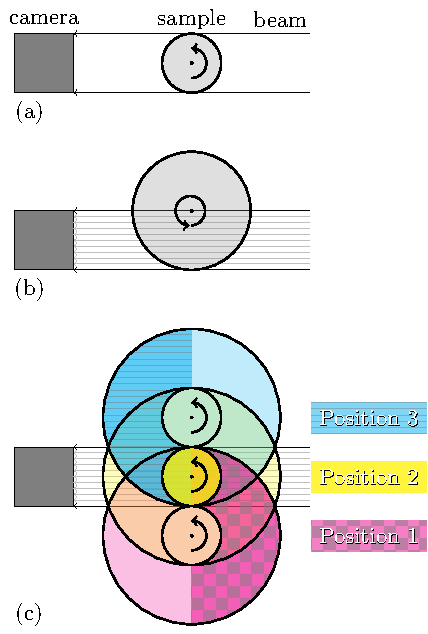
\includegraphics{img/Haberthuer2010/Fig01-FOV}
	\caption[Covering the field of view of differently sized samples]{Covering the field of view of differently sized samples with one \SI{180}{\degree} scan (a), one \SI{360}{\degree} scan (b) or---in the case of the so called wide field scanning---with multiple subscans (three subscans, c). The filled segments mark the region of the sample that is covered while scanning the respective positions (Position 1: magenta/checkerboard, Position 2: yellow, Position 3: cyan/striped).}
	\label{fig:scanning-possibilities}
\end{figure}

For tomographic scans covering a size wider than two fields of view, three or more \SI{180}{\degree}-scans taken at slightly overlapping positions are combined, as shown in Figure~\ref{fig:scanning-possibilities}(c). The projections of each subscan overlap slightly to facilitate the stitching of multiple projections into a single one. The cutline, i.\,e. the position where the merging takes place, is automatically determined according to a mean squared difference method~\cite{Hintermueller2010}.

A straightforward acquisition scheme would record an equal amount of projections for each of the individual subscans. As a consequence, to fulfill the sampling theorem in the lateral parts of the sample, oversampling the central parts of the sample would be necessary.

Since the total acquisition time per sample linearly scales with the total amount of recorded projections such an acquisition scheme obviously increases the total amount of beamtime for one sample without relevantly increasing the quality of the reconstructed tomographic data. Hence, such an oversampling is generally avoided.

Our goal was to find a good compromise between scanning time and image quality. We therefore devised an acquisition scheme for covering a wide field of view based on the assumption that a sufficient resolution and contrast can be achieved in the tomographic dataset, if the sampling theorem is individually fulfilled for each of the subscans. This results in a set of $i$ subscans with $P_{i}$ projections each. A simple example with $P_{2}=4$ and $P_{1}=P_{3}=8$ is shown in Figure~\ref{fig:projections}(a). Since each subscan $i$ has a different number of projections $P_{i}$, the stitching algorithm has to interpolate missing projections from adjacent projections (represented by the dotted lines in Figure~\ref{fig:projections}(b)) to generate a complete set of merged projections for reconstruction.

As a by-product, such an optimization of the individual number of projections $P_{i}$ for each subscan $i$ decreases the total acquisition time for one sample and thus the imparted radiation dose.

\begin{figure}[htb]
	\centering
	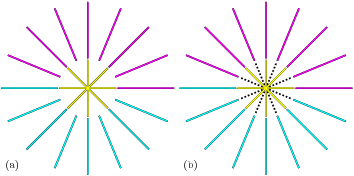
\includegraphics[width=\imsize]{img/Haberthuer2010/Fig02-Interpolation}
	\caption[Wide field scan setup]{Wide field scan setup with three \SI{180}{\degree} scans; one central (yellow) and two lateral scans (magenta and cyan or top and bottom, respectively). In this drawing, four projections for the central and eight projections for each of the lateral scans have been recorded. The colors of the three positions correspond to the colors shown in Figure~\ref{fig:scanning-possibilities}(c). %
	(a): scanned projections %
	(b): scanned projections and additional interpolated projections (dotted) required to merge all projections.}
	\label{fig:projections}
\end{figure}	

We defined a gold standard protocol and several additional scanning protocols in order to compare different acquisition schemes. The gold standard protocol covers the desired field of view while fulfilling the sampling theorem---which states that for a detector width of $D$ pixels, we need to acquire a number of projections $P=D\frac{\pi}{2}$~\cite{Kak2002}---in all its regions, as shown in Figure~\ref{fig:SubScan-Setup}(a). In this case we need to achieve a field of view of 3072 pixels. The dark gray circle is the field of view that could be covered using a large detector with a size of 3072 pixels and recording $P=3072\frac{\pi}{2}=4825$ projections.

Using a detector with a size of 1024 pixels, this desired field of view could be covered with nine independent local tomography scans. Such an approach would require nine independent reconstructions and stitching of those nine reconstructed tomographic datasets into one dataset covering the full field of view. This method would also introduce artifacts at the edges of each of the nine sub-datasets which would lie inside the sample to be imaged.

While the chosen field of view of 3072$\times$3072 pixels can be covered using a detector of the size of 3072 pixels in one scan, we can cover the desired field of view with a much smaller detector, using a scanning protocol with three subscans from which we obtain merged projections. Figure~\ref{fig:SubScan-Setup}(b) shows how the desired field of view of 3072 pixels can be covered with a wide field scan, composed of one central and two half ring-scans, recorded with a small detector with a size of 1024 pixels and 4825 projections per subscan (a total of 14475 projections) which are then subsequently merged to 4825 large projections spanning the whole field of view. A further increase in the field of view can be obtained by simple iteration. Figures~\ref{fig:SubScan-Setup}(c)--(f) show such a setup for a five- or seven-fold increase.

\begin{figure}[p]
	\centering
	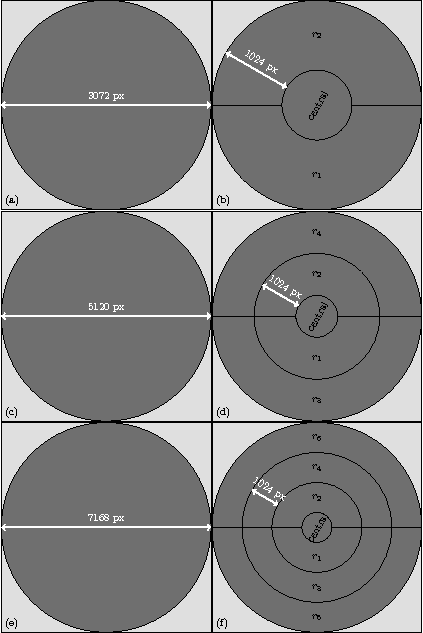
\includegraphics[width=.8\linewidth]{img/Haberthuer2010/Fig03-3-5-7}
	\caption[Setup for different field of views]{Setup for different field of views. %
		(a): Desired field of view of 3072 pixel diameter. %
		(b): Wide field scanning protocol for covering the desired field of view of panel (a) with merged projections from one central and two half ring scans ($r_{1}$ and $r_{2}$). %
		(c): Desired field of view of 5120 pixel diameter. %
		(d): Wide field scanning protocol for covering the desired field of view of panel (c) with merged projections from one central and four half ring scans ($r_{1}$--$r_{4}$). %
		(e): Desired field of view of 7168 pixel diameter. %
		(f): Wide field scanning protocol for covering the desired field of view of panel (e) with merged projections from one central and six half ring scans ($r_{1}$--$r_{6}$).}%
	\label{fig:SubScan-Setup}
\end{figure}

\subsection{Quality guided protocols}\label{sec:quality guided protocols}
Taking the experimental constraints like desired field of view, available detector size, magnification and binning into account, a MATLAB-script calculates a set of acquisition protocols. Each such protocol contains the number of projections for each subscan linearly scaled in total amount of projections from a gold standard scan down to a protocol where the sampling theorem is far from being satisfied (Table~\ref{tab:protocols}). Through optimization of the number of recorded projections, a reduction of the total acquisition time by \SI{84}{\percent} (compared to the gold standard) was achieved.

Using a Shepp-Logan phantom~\cite{Shepp1974} with added Gaussian noise as a reference image, a simulated tomographic scan and subsequent reconstruction was calculated for each of these acquisition protocols. For each protocol we calculated the expected reconstruction quality using the difference image between the reconstruction of this protocol and the initial reference image. This simulated reconstruction quality was plotted against the total acquisition time (red dots in Figure~\ref{fig:NormalizedErrorPlot}).

The end-user---balancing between acquisition time and desired image quality---chooses one protocol from the presented set for scanning his sample. A file containing all the details of the chosen scan is written to disk, and parsed by a custom Python-script. This script interacts with the hardware control system at the \ac{tomcat} beamline enabling an automated, unattended batch acquisition of all necessary subscans.

To assess the simulations in a real world example, we selected nineteen different acquisition protocols with varying number of projections to scan one single sample (details are specified in Table~\ref{tab:protocols}, including the calculated Quality for each protocol).

A scan covering the chosen field of view with nine independent local tomography scans, each with a field of view of 1024$\times$1024 pixels, would need a total of $P=9(1024\frac{\pi}{2})=14476$ projections. This protocol was not considered for this study, since the sampling theorem can be equally satisfied by acquiring the required amount of projections with one central and two ring scans, as defined in section~\ref{subsec:increasing the field of view}. Including an overlap of 100 pixels between the central and the ring scan, an equivalent wide field scanning protocol (Protocol A in Table~\ref{tab:protocols}) requires the acquisition of 13534 projections ($P_{A}=3(3072-200)\frac{\pi}{2}$).

Protocols B--T have been linearly scaled down with a decreasing number of acquired projections of the ring scans. To simplify interpolation and merging of the projections from each subscan, we only selected acquisition schemes where the number of projections of the inner and the outer subscans is the same or a multiple of two (see figure~\ref{fig:projections}). This constraint also led to a slight oversampling for protocol B, otherwise the number of projections for each subscan of this protocol ($5244=3\cdot874$) would not have scaled down nicely to the 874 projections used for protocol T.

All parameters of each protocol and each subscan (sample-position in relation to the beam, rotation angles and number of projections) were set in a preference-file, generated using aforementioned MATLAB-script. One rat lung sample was scanned using each of the 19 different protocols (B--T), without manual intervention, permitting a direct comparison of the reconstructed datasets.

\begin{threeparttable}
	\caption[Details of the 19 scanned protocols]{Details of the 19 scanned protocols for this study (B--T): An unoptimized scan to cover the desired field of view of 3072 pixels with nine independent scans (with a detector width of 1024 pixels) would require to record a total of $P_{\textrm{Gold standard}}=9(1024)\frac{\pi}{2}=14476$ projections. The wide field scanning protocol (A) equivalent to this field of view only uses three subscans, resulting in a total number of projections of $P_{A} = 3(3072-200)\frac{\pi}{2}= 13534$. Three-dimensional reconstructions of the datasets marked with a light gray background are shown in Figure~\ref{fig:BvsT}.}
	\label{tab:protocols}
	\begin{tabular}{ccccccc}
		\toprule
		\multirow{2}{*}{Protocol} & \multicolumn{3}{c}{Projections for Subscan} & Total Number & Time/Radiation & Simulated\\
			& $\textrm{s}_{1}$ & $\textrm{s}_{2}$ & $\textrm{s}_{3}$        & of Projections & Dose [\%] & Quality [\%]\\
		\midrule
		A\tnote{1} & & & & 13534 & 100 & \\
		\rowcolor{lightgray} B\tnote{2} & 5244 & 5244 & 5244 & 15732 & 116 & 100\\
		C & 5244 & 2622 & 5244 & 13110 &  97 & 89\\
		D & 4370 & 4370 & 4370 & 13110 &  97 & 85\\
		E & 4370 & 2185 & 4370 & 10925 &  81 & 87\\
		F & 3934 & 3934 & 3934 & 11802 &  87 & 80\\
		G & 3934 & 1967 & 3934 & 9835  &  73 & 84\\
		H & 3496 & 3496 & 3496 & 10488 &  77 & 78\\
		I & 3496 & 1748 & 3496 & 8740  &  65 & 80\\
		J & 3060 & 3060 & 3060 & 9180  &  68 & 76\\
		K & 3060 & 1530 & 3060 & 7650  &  57 & 75\\
		\rowcolor{lightgray} L  & 2622 & 2622 & 2622 & 7866  &  58 & 72\\
		M & 2622 & 1311 & 2622 & 6555  &  48 & 69\\
		N & 2186 & 2186 & 2186 & 6558  &  48 & 67\\
		O & 2185 & 1093 & 2185 & 5463  &  40 & 62\\
		P & 1748 & 1748 & 1748 & 5244  &  39 & 61\\
		Q & 1748 & 874  & 1748 & 4370  &  32 & 55\\
		R & 1312 & 1312 & 1312 & 3936  &  29 & 46\\
		S & 874  & 874  & 874  & 2622  &  19 & 21\\
		\rowcolor{lightgray} T & 874  & 437  & 874  & 2185  &  16  & 20\\
		\bottomrule
	\end{tabular}
	\begin{tablenotes}
		\footnotesize
		\item[1] Wide field scan equivalent to an unoptimized scan covering the field of view with nine independent scans.
		\item[2] Gold Standard for this study
	\end{tablenotes}

\end{threeparttable}

\subsection{Projection merging and tomographic reconstruction}
After acquisition of the three subscans per protocol, custom MATLAB functions read the parameters of the single subscans (e.\,g. sample name, amount of subscans, amount of dark and flat images) as well as the desired output-name and -suffix, and performed all necessary calculations, including: loading of the correct projections from each subscan; normalizing; interpolation; cutline detection; correct stitching of the images into wide field projections, and writing these merged projections as well as log files needed for the reconstruction to disk.

The merged projections were subsequently rearranged into sinograms, where the $n$\textsuperscript{th} sinogram is composed of the $n$\textsuperscript{th} line of every corrected projection. The $n$\textsuperscript{th} slice of the tomographic scan was reconstructed from the $n$\textsuperscript{th} sinogram using an \acs{fft}-based regridding algorithm~\cite{Dowd1999,Marone2008}. The 19 tomographic datasets were reconstructed on a computing cluster composed of five \SI{64}{\bit} Opteron machines with four cores and \SI{8}{\giga\byte} \acs{ram} each. The reconstructions resulted in an image stack covering a large sample volume of 2792$\times$2792$\times$1024 pixels, a nine-fold increase from the standard volume of 1024$\times$1024$\times$1024 pixels for one conventional scan.

\section{Results}\label{sec:Results}
\subsection{Image Merging and Reconstruction}\label{sec:Image Merging and Reconstruction}
Figure~\ref{fig:wide-field-scan-results}(a) shows corrected projections from three overlapping subscans prior to merging, including regions where the subscans are overlapping. Figure~\ref{fig:wide-field-scan-results}(b) shows one merged projection prior to reconstruction and Figure~\ref{fig:wide-field-scan-results}(c) shows one slice of the reconstructed dataset. The example shown in Figure~\ref{fig:wide-field-scan-results} was obtained using the highest number of projections and is therefore protocol B. One reconstructed slice covers a field of view of 2792$\times$2792 pixels (4.13$\times$\SI{4.13}{\milli\meter}), which is almost three times the size of what can be achieved with one single binned scan (1024 pixels or \SI{1.52}{\milli\meter}). %1024 * 1.48 um/px = 1.51552mm
The dashed circles on the reconstructed slice mark the start and the end of the overlap region.

\begin{figure}[p]
	\centering
	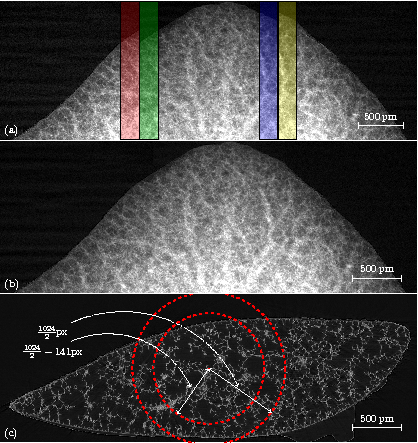
\includegraphics[width=\linewidth]{img/Haberthuer2010/Fig04-Workflow}
	\caption[Workflow of a wide field scan]{Workflow of a wide field scan. The images show a rat lung sample from a Sprague-Dawley rat, obtained 21 days after birth, scanned with the acquisition protocol B (Table~\ref{tab:protocols}). %
			(a): Three corrected and independently acquired projections from subscans $s_1$--$s_3$ are shown. Each one is 1024\(\times\)1024 pixels large and covers a field of view of \SI{1.52}{\milli\meter}. Subscans $s_1$ and $s_2$ overlap by 141 pixels (red and green overlay), subscans $s_2$ and $s_3$ overlap by 138 pixels (blue and yellow overlay). %
			(b): Merged projection obtained from the three subscans shown in subfigure (a). Each merged projection has a size of 2792\(\times\)1024 pixels. Due to the overlap required to merge the projections, the width of the merged projections is slightly smaller than three times the width of the subscans. %
			(c): Cropped slice of the reconstructed tomographic dataset. The dashed red circles mark the start and end of the overlap region.}
	\label{fig:wide-field-scan-results}
\end{figure}

Figure~\ref{fig:s2-wfs} shows the advantages of the wide field acquisition scheme. With---in this particular case---an enlargement of the field of view by almost a factor of three, it is possible to visualize entire acini at high resolution. For a conventional scan (fig.~\ref{fig:s2-wfs}(a)), the airway segments in the sample are only partially contained inside the dataset (magenta and yellow). The semitransparent airway segments are contained in the sample, but are not visible in the field of view of a dataset obtained with a conventional scan. Increasing the field of view (fig.~\ref{fig:s2-wfs}(b)) allows the visualization of those segments to their full extent. A third acinus (cyan) which was not visible in Figure~\ref{fig:s2-wfs}(a) can now easily be visualized.

\begin{figure}[p]
	\centering
	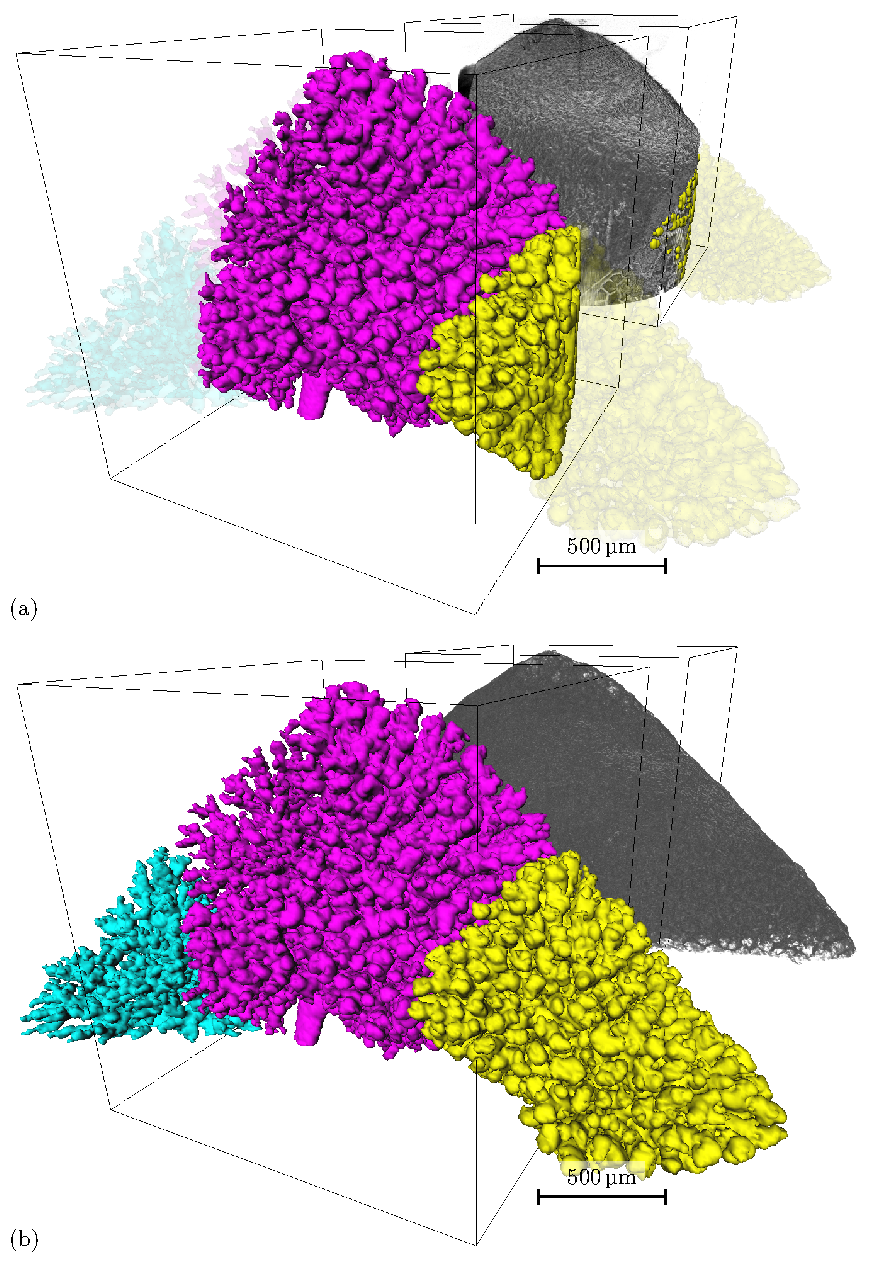
\includegraphics[width=.7\linewidth]{img/Haberthuer2010/Fig05-ConvVsWfs}
	\caption[Three-dimensional visualization of the distal-medial tip of the right lower rat lung lobe]{Three-dimensional visualization of the distal-medial tip of the right lower rat lung lobe. The gray structure in the background shows a semitransparent view of the tomographic dataset with segmented airways. The foreground shows isosurfaces of terminal airways. The wireframe cube has a side length of 1024 pixels and encloses the field of view of one conventional scan. %
	(a): Conventional scan; the extracted airway segments (magenta and yellow or left and right, respectively) are only partially contained inside the total sample volume. Airway segments not contained in the dataset, but present in the sample are shown semitransparent. This conventional scan corresponds to a reconstruction of the central of the three wide field scan subscans. %
	(b): Wide field scan with increased field of view; the magenta (center) and yellow segment (right) show entire acini inside the dataset, the cyan segment (left) contains a partially cut acinus. All airway segments inside the sample are contained in the tomographic dataset.}
	\label{fig:s2-wfs}
\end{figure}

\subsection{Performance of the scanned protocols}
The performance of the 19 protocols has been quantified using the difference image between binarized slices of the gold standard protocol and each protocol to be assessed. The slices have been thresholded according to \citet{Otsu1979}. The difference value ($E_{norm}$) plotted in Figure~\ref{fig:NormalizedErrorPlot} was calculated for each protocol $i=$1--19 (B--T) according to equations~\ref{eq:errorcalculation-a}--\ref{eq:errorcalculation-c}. Using a thresholded slice $k$ of each protocol $i$ ($Slice_{i_{k}}$) and the corresponding slice $k$ of the gold standard protocol $B$ ($Slice_{B_{k}}$) the absolute difference image ($D_{i_{k}}$) of these two slices $k$ was calculated. The sum of all pixels of this difference image yields a value ($E_{i_{norm_{k}}}$) for the difference of the examined slice $k$ of protocol $i$ with the corresponding slice of the gold standard protocol B.
\begin{eqnarray}
	D_{i_{k}} &=& |Slice_{B_{k}}-Slice_{i_{k}}|\label{eq:errorcalculation-a}\\%
	E_{i_{norm_{k}}} &=& \sum_{x}\sum_{y} D_{i_{k}}\label{eq:errorcalculation-b}\\%
	E_{i_{norm}} &=& \overline{E_{i_{norm_{k}}}}\label{eq:errorcalculation-c}%
\end{eqnarray}

This combined difference value ($E_{i_{norm_{k}}}$) was calculated for 205 regularly spaced slices (%
%$i=1:5:1024$%
every fifth slice) of the full dataset. The mean ($\overline{E_{i_{norm_{k}}}}$) difference value for all slices was normalized to the scanned quality-steps from 16--\SI{116}{\percent} (as stated in Table~\ref{tab:protocols}) and plotted with its standard deviation ($\sigma(E_{i_{norm_{k}}})$). For the purpose of comparison, data has been normalized.

As expected, the calculated quality of the reconstructions representing the different protocols decreases as a function of total number of obtained projections (Figure~\ref{fig:NormalizedErrorPlot}). The calculated error of the different protocols (normalized difference value, blue diamonds) shows the experimental results obtained from actual scans of lung tissue. The plots for the simulation as defined in section~\ref{sec:quality guided protocols} (red dots) and the normalized difference value are not perfectly in agreement, but show the same trend. The linear regression for the simulation shows a steeper decrease for the quality ($y_{Sim}=0.6936x+26.891$) than the linear interpolation for the experimental data ($y_{Exp}=0.5833x+20.226$). The linear regression coefficient for both the linear interpolations are comparable ($R^{2}_{Sim}=0.8287$, $R^{2}_{Exp}=0.7868$).

\begin{figure}[htb]
	\centering
	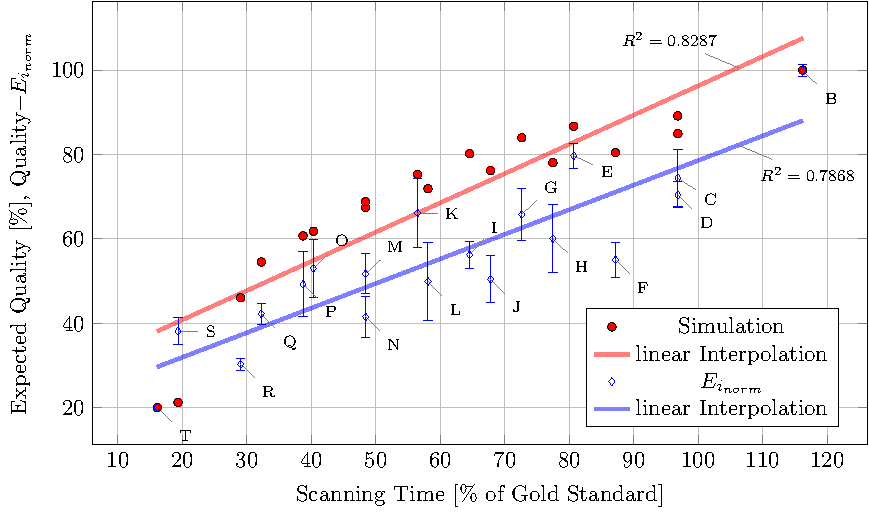
\includegraphics[width=\linewidth]{img/Haberthuer2010/Fig06-Plot}
	\caption[Plot of normalized difference Value for the scanned protocols overlaid over Quality-plot obtained from the simulation]{Plot of normalized difference Value ($E_{i_{norm}}$, blue diamonds) for the 19 scanned protocols overlaid over Quality-plot (red dots) obtained from the simulation (described in section~\ref{sec:quality guided protocols}. The normalized Error has been calculated using the difference image of each protocol $i$ with protocol B. The error bars for each protocol show the standard deviation of the error calculated for 205 of the 1024 slices. Note that the scale of the error was normalized to 20--\SI{100}{\percent}, so that both the quality from the simulation and the error are directly comparable. The abscissa shows the scanning time in percentage of time used for the gold standard scan. Protocol T on the far left corresponds to the fastest scanning time, protocol B on the far right to the slowest. The protocols in between are shown from T--B for increasing percentage of the scanning time.}
	\label{fig:NormalizedErrorPlot}
\end{figure}

\subsection{Three-dimensional visualization of different protocols}
\label{subsec:comparison}
The tomograms of the different protocols were three-dimensionally analyzed and visualized using MeVisLab (Version 2.0 (2009-06-09 Release), MeVis Medical Solutions AG and Fraunhofer MEVIS - Institute for Medical Image Computing, Bremen, Germany). Airway segments were extracted using a threshold interval based region growing algorithm~\cite{Zucker1976}. A seed point for the region growing algorithm was manually defined in the most proximal slice for each independent airway segment. The coordinates of the seed points were kept constant for protocol B--T, allowing direct comparison between the airway segment reconstructions of the different protocols. Airway segments extracted for protocol B, L and T are shown in Figure~\ref{fig:BvsT}.

Protocol B corresponds to a slightly oversampled gold standard scan, obtained with total 15732 projections, recorded in \SI{66}{\minute}. Protocol L was obtained in \SI{35}{\minute} with total 7866 projections. Protocol T was obtained in \SI{12}{\minute} with 2185 projections for all three subscans. The tomographic dataset from protocol B was reconstructed from 5244 merged projections, the dataset from protocol L was reconstructed from 2622 merged projections and the dataset from protocol T was reconstructed using only 874 merged projections. Even though protocols L and T were scanned while violating the sampling theorem and with a total scanning time reduction of \SI{40}{\percent} (L) or more than \SI{86}{\percent} (T), the samples still appear to be identical to the gold standard protocol in the low-resolution three-dimensional visualizations shown in Figure~\ref{fig:BvsT}(a)--(c).

Figure~\ref{fig:BvsT}(d)--(f) show isosurface visualizations of the border between airspace and lung tissue as cubic regions of interest (256 pixels wide, location inside the sample is marked as blue cube in Figure~\ref{fig:BvsT}(a)--(c)). Because of experimental constraints, the cutline between the individual subscans could not be defined with a precision of one single pixel. As a consequence, the clipping plane does not lie in exactly the same position. This explains the appearing and disappearing holes in Figure~\ref{fig:BvsT}(d)--(f).

Even with the higher magnification, the reconstruction of protocol L in Figure~\ref{fig:BvsT}(e) appears nearly identical to the reconstruction of the region of interest of protocol B (fig.~\ref{fig:BvsT}(d)). The isosurface of the region of interest of protocol T shown in Figure~\ref{fig:BvsT}(f) appears rougher than the isosurface of protocol B. This roughness is introduced through ray-like artifacts visible in the original slice of the dataset of protocol T (not shown). These artifacts are the consequence of a strong subsampling. With the acquisition of only 874 projections instead of the required 5139, the sampling theorem is far from being satisfied. However, even with this strong undersampling, segmentation, three-dimensional reconstruction and visualization of the sample is still possible.

\begin{figure}[htb]
	\centering
	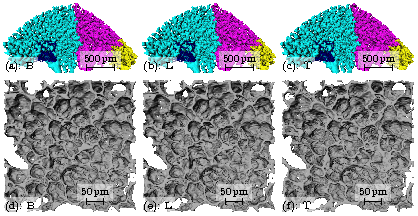
\includegraphics[width=\linewidth]{img/Haberthuer2010/Fig07-B-L-T}
	\caption[Comparison of three-dimensional visualizations]{Comparison of three-dimensional visualizations. %
			(a)--(c): Three independent airway segments (cyan, magenta, yellow) of tomographic datasets obtained with protocol B, L and T, extracted using a region growing algorithm. A cubic region of interest (blue) with a side length of 256 pixels (corresponding to \SI{379}{\micro\meter}) is marked inside the leftmost segment for all protocols. %
			(d)--(f): Detailed view of isosurfaces of the lung tissue inside the blue \acp{roi} for protocol B, L and T, respectively. Note the increasing surface roughness in the alveolar surfaces for subfigures (e) and (f).}%
	\label{fig:BvsT}
\end{figure}%
%\twocolumn%

For further analysis four regions of interest with a side length of 256 pixels have been extracted for each of the protocols B, L and T. The three-dimensional location of these \acp{roi} inside the sample is shown in Figure~\ref{fig:roi3d}.

\begin{figure}[htb]
	\centering
	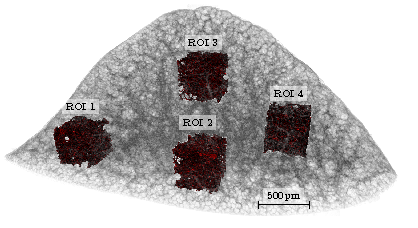
\includegraphics[width=\linewidth]{img/Haberthuer2010/Fig08-ROIs}
	\caption[Overview of the location of the four regions of interest in the sample]{Overview of the location of the four regions of interest where the histogram of the euclidean distance transformation distribution has been calculated. Grey: Semitransparent volume rendering of the lung tissue sample. Red: Four regions of interest, extracted to calculate the distance transformation. The labels of the \acp{roi} conform to the legends in Figure~\ref{fig:DTFplots}.}%
	\label{fig:roi3d}
\end{figure}

Each of the \acp{roi} has been binarized using an algorithmically determined threshold~\cite{Otsu1979} and small particles inside the segmented airspace lumen have been removed using a connected component analysis. Subsequently, the euclidean distance transformation~\cite{Danielsson1980} has been calculated for each thresholded \ac{roi}.

For comparison, the histogram of the euclidean distance transformation has been plotted for all four regions of interest in each protocol (B, L and T).

\begin{figure}[htb]
	\centering
	\includegraphics[width=\linewidth]{img/Haberthuer2010/Fig09-DTF}
	\caption[Histogram-Plots]{Histogram-Plots for each of the of four \acp{roi}, each showing the histogram of the distance transformation for the protocols B, L and T.}%
	\label{fig:DTFplots}
\end{figure}

Figure~\ref{fig:DTFplots} shows logarithmic plots of the histogram distributions for the four selected \acp{roi}; the blue, green and red plot show the histograms of the distance transformation of Protocol B, L and T, respectively. For all four regions of interest, the distribution of the euclidean distance transformation is very similar, only for larger airway diameters (between 50--\SI{60}{\micro\meter}) we see a detectable difference in the regions of interest 1 and 4, located in the lateral parts of the sample. If we remember that the histogram is plotted with a logarithmic y-axis, we see that the difference of the histograms is only visible for several hundred voxels.

Even when reducing the sample acquisition time by \SI{84}{\percent} of the gold standard scan (T vs. B), the distance transformation histograms of the shown regions of interest are very similar and therefore no relevant structural differences are introduced.

As a further proof of concept we scanned and reconstructed a rat lung sample with five scanning positions, resulting in a nearly five-fold (4.74$\times$) increase in field of view from slices with a size of 1024$\times$1024 pixels to a size of 4852$\times$4852 pixels (1.52$\times$\SI{1.52}{\milli\meter} to 7.18$\times$\SI{7.18}{\milli\meter}) at a voxel side length of \SI{1.48}{\micro\meter}. A three-dimensional visualization of the boundary between airspace and tissue in this reconstructed dataset validated the wide field scanning method for further increases in the available field of view (data not shown).

\section{Discussion}\label{sec:Discussion}
We present a method to laterally increase the field of view of tomographic imaging systems operated in parallel beam geometry and would like to call this method \ac{wf-srxtm}. We defined scanning protocols for the optimization of the total imaging time versus the expected imaging quality, enabling a very fast acquisition of lower quality tomographic datasets, or acquisition of very high quality datasets in a longer time.

Even if the reduction in scanning time does introduce minor artifacts in the three-dimensional reconstruction, as shown in Figure~\ref{fig:BvsT}, an automated segmentation of the relevant features in the sample is still possible, even for protocols with greatly reduced scanning time. 

Additionally, shortening the scanning time also reduces the radiation damage even though, for this study, this was not an issue. Obviously, a reduction of the imparted dose to the sample is crucial when radiation sensitive sample are investigated. With a
suitable protocol the dose can be reduced by \SI{84}{\percent} (Table~\ref{tab:protocols}), which might be a significant step towards tomographic imaging of sensitive samples using ultra high resolution and enhanced field of view. 

The field of view was increased three-fold by merging projections from three partially overlapping scans and reconstructing these resulting projections using the standard workflow at the \ac{tomcat} beamline (Figure~\ref{fig:wide-field-scan-results}). As a consequence of the sampling theorem, an increased amount of projections had to be acquired, thus increasing the acquisition time. To overcome this limitation, we defined multiple scanning protocols with a reduced amount of total projections and thus reduced acquisition time and delivered dose (Table~\ref{tab:protocols}). All of these protocols were evaluated for the quality of the resulting reconstructions and compared to a gold standard scan. We have shown that the resulting quality can be simulated prior to scanning and thus provide a tool to choose a suited scanning protocol, based on the demands for scanning time optimization and quality of the resulting tomographic dataset (Figure~\ref{fig:NormalizedErrorPlot}). 

Reducing the amount of projections for the central of the three subscans may be performed with a minor loss of fidelity in the resulting reconstructions. Let us compare protocols D/E and H/I. For protocols E and I we acquired half the amount of projections for the central subscan $\textrm{s}_{2}$ as compared to protocols D and H. In both cases we reduce the scanning time by \SI{17}{\percent}, but keep the quality of the scan on a comparable level (D: $\SI{70}{\percent}\pm3.09$ vs. E: $\SI{80}{\percent}\pm3.01$, H: $\SI{60}{\percent}\pm8.08$ vs. I: $\SI{56}{\percent}\pm3.23$).
% B--C = 13110/15732 = 0.8333, 100%--89%
% D--E = 10925/13110 = 0.8333, 85%--87%
% H--I = 8740/10488 = 0.8303; 78%--80%
We show that the interpolation of missing projections does not introduce relevant errors in the resulting tomographic datasets.

For protocols with an equal amount of total projections, but differing amount of projections for the individual subscans (C/D and M/N) we observed minor differences in reconstruction quality. The qualities $E_{i_{norm}}$ of protocols C and D lie within their respective standard deviation ($\SI{74}{\percent}\pm6.81$ vs. $\SI{70}{\percent}\pm3.09$), and the qualities of protocols M and N are comparable ($\SI{52}{\percent}\pm4.71$ vs. $\SI{42}{\percent}\pm4.78$). Both protocols C and M are scanned without oversampling the central subscan, making interpolation necessary, for protocols D and N we simply stitched the projections of the three subscans. Note that for protocol N we do undersample the outer parts of the sample. When deciding between two protocols with the same amount of total projections, it is thus desirable to favor the protocol where the central scan is not oversampled (i.\,e. choosing protocol C instead of D). Even if this introduces additional computing time to interpolate projections prior to reconstruction, these protocols show an increased quality compared to protocols where the central scan is oversampled. Since an oversampling of the central scan does not add much to the total reconstruction quality and the outer parts of the sample contribute more to the total area of the projections, choosing a protocol where the sampling theorem is satisfied better for those parts of the sample is favorable (i.\,e. favouring protocol M to protocol N).

With the defined protocols we open the possibility for the end-user to choose an acquisition mode suited to fulfill the constraints on number of samples to be scanned within the allocated beamtime and desired quality of the reconstructed datasets.

Additionally, two special use-cases for different protocols are worth mentioning. First, if the user needs a very quick overview over samples at high resolution, a time-saving protocol can be used. This is especially the case, if the integrity of the sample can only be judged with a tomographic scan. Based on the quick scan the right samples for high resolution scans may be selected. It has to be mentioned that a quick overview could---in principle---be obtained with a low-resolution scan, which usually automatically accommodates a larger field of view. However, the resolution of such an overview scan is not always sufficient to detect interesting features in the samples which might be damaged.

We have shown that the field of view of parallel beam tomographic end-stations can be increased up to five-fold and have routinely reconstructed multiple tomograms with a three-fold increase in field of view. The shown acquisition protocols are theoretically expandable for more than five subscans, although the reconstruction of wide field scans with seven or more subscans would require an extremely powerful data processing infrastructure. The datasets shown in Figure~\ref{fig:BvsT} are binned scans resulting in datasets of 1024 slices, each with a size of 2792$\times$2792 pixels at \SI{8}{\bit} gray value depth, which adds up to a total size of the dataset of approximately \SI{7.5}{\giga\byte}. If we assume an unbinned scan with seven overlapping subscans, the size of one stitched projection will be approximately 14000$\times$14000 pixels. The full dataset will consist of 2048 such slices, which would add up to a total size for the full dataset of approximately \SI{383}{\giga\byte}.

Even if the amount of data to handle is huge, a wide field scan with a five-fold increase in field of view remains interesting, since it would enable the end-user to selectively reconstruct only regions of interest from large samples with ultra-high resolution. Up to now, a two-step process was required to scan precisely defined regions from samples larger than the field of view. This process involved the use of different magnifications, two separate beamtimes and a precise registration of the samples between those beamtimes.

\section{Summary}\label{summary}
A method to increase the lateral field of view of tomographic imaging has been established, which enables the high-resolution tomographic imaging of large samples that are wider than the field of view of the optical setup in multiple semi-automatically combined steps. Tomographic datasets of entire rat lung acini have been acquired with an enhanced field of view using \ac{wf-srxtm}.

Different optimized scanning protocols for covering a large field of view have been validated and are now provided for the end-users of the \ac{tomcat} beamline. End-users now have the possibility to choose suitable scanning protocols depending on a balance between acquisition time and expected reconstruction quality. Depending on this balance, a reduction of the image acquisition time by \SI{84}{\percent} is possible, while keeping the quality of the reconstructed tomographic dataset on a level still permitting automated segmentation of the lung structure and surrounding airspace, as shown in section~\ref{subsec:comparison}. The reduction in acquisition time obviously reduces the time during which the sample is irradiated by synchrotron radiation and thus reduces the radiation dose inflicted on the sample.

\section{Acknowledgments}
This work has been funded by the grants 3100A0-109874 and 310030-125397 of the Swiss National Science Foundation. We thank Mohammed Ouanella for his excellent technical assistance and Volker Dicken from Fraunhofer MEVIS for the fruitful discussion concerning the euclidean distance transformation. Dan Ward kindly checked the English of the manuscript.
%\bibliographystyle{plainnat}
%\label{app:bibliography} 
%\bibliography{../Bibliography,../../references,../Tsuda2008references}
%%%%%%%%%%%%%%%%%%%%%%
\cleardoublepage\myPart{Discussion \& Outlook}\label{part:discussion}
% !TEX root = ../Thesis.tex
\acresetall
\myChapter{Discussion}\label{ch:discussion}
\begin{flushright}{\slshape And as soon as I'm done with these waffles, I shall discuss my evil plan!} \\ \medskip
	--- \defcitealias{Zim}{Invader Zim}\citetalias{Zim} \citep{Zim}
\end{flushright}

\vfill

The tomographic data obtained at the beamline for \ac{tomcat} offers an unmatched three-dimensional insight into the mammalian lung. Even if higher resolution images of the terminal airway ends than the ones obtained at \ac{tomcat} have been obtained with scanning \ac{em}\todo{citation/nice image? $\rightarrow$ Dani Studer?}, these images only provide a view of the surface structure of a sample and are not suited for a full three-dimensional reconstruction of the terminal airway ends. Using standard \ac{em} is impossible to visualize the larger three-dimensional structure of the terminal airway ends inside the lung since the sample has to be sectioned prior to acquiring images using this method, which essentially destroys the full three-dimensional information and makes it impossible to reconstruct larger volumes of the lung structure\todo{mention \threed \ac{em}-tomography?}

Tomography in contrast offers a non-destructive insight into the lung, tomographic microscopy using \ac{uct} enables the study of the major airways of swine~\cite{Litzlbauer2006}, rat~\cite{Langheinrich2004a,Sharif2010} or mice lung~\cite{Langheinrich2004,Ritman2005} and while \ac{srxtm} and \ac{wf-srxtm} enable the study of the functional lung units of the lung, the so-called acini with unmatched resolution and precision.

In this work three imaging methods based on ultrahigh resolution tomographic data of the terminal airway have been presented, the following sections discuss the major notable points of each of them.

\section{Multimodal Imaging}
The method presented in \autoref{ch:xrm2008} combines the advantages of tomographic imaging and \ac{em} into a multimodal imaging approach for the analysis of inhaled particles in the lung. The tomographic data provides the unrestricted three-dimensional information on the location of sub-micron particles in the terminal airway tree which is combined with the extremely high resolution of the \ac{em}-images for the precise analysis of those particles in the lung tissue.

Exposure to ultra-fine particles and nanoparticles produces by environmental or industrial sources is an important health problem. It is expected that inhaled particles are deposited in specific locations in the lung\todo{citation $\rightarrow$ Christian Mühlfeld, Barbara Rothen?}. With currently available methods, the exact location of these deposition sites in relation to the airways tree cannot easily be analyzed. 

Classic histological sections analyzed using light and electron microscopy allow for a precise location of the inhaled particles in relation to the tissue, \ie make it possible to analyze the interaction of the particles with alveolar macrophages and epithelial cells~\cite{Muhlfeld2008}. But the precise localization of these interaction sites inside the airway tree are impossible to extract using histological sections since the three-dimensional structure of the sample is destroyed.

Registration of classic histological slices with the three-dimensional data obtained through \ac{srxtm} make it possible to localize sites of interaction along the airway tree inside the three-dimensional structure of the terminal airways. The method presented in \autoref{ch:xrm2008} was only little more than a proof of concept in terms of the registration between the two imaging modalities. Careful alignment of the sample prior to physical sectioning made registration straightforward, since the images only needed to be corrected for rotation and translation to be able correlate between a physical slice imaged using \ac{em} and a virtual slice of the \ac{srxtm} dataset.

\autoref{fig:correlation} shows the three-dimensional situation of different alignment situations of the two multimodal datasets. The situation shown in \autoref{subfig:correlation-planar} can be achieved through careful alignment of the sample prior to histological sectioning and corresponds to the situation presented in \autoref{ch:xrm2008}. The fully unrestricted three-dimensional information of the airway tree can be matched with highest resolution two-dimensional information about the particle location in or around the tissue in the lung.

Figures~\ref{subfig:correlation-arbitrary1} and \ref{subfig:correlation-arbitrary3} depict situations where the two datasets are arbitrarily orientated with one or multiple degrees of rotation, respectively.

\renewcommand{\imsize}{\linewidth}%
\begin{figure}[p]
	\centering%
	\pgfmathsetlength{\imagewidth}{\imsize}%
	\pgfmathsetlength{\imagescale}{\imagewidth/1586}%
	\def\x{1160}%
	\def\y{364}% scalebar-y at 90% of height of y=404px
	\subfloat[Planar orientation of slice]{%
		\begin{tikzpicture}[x=\imagescale,y=-\imagescale]%
			\node[anchor=north west, inner sep=0pt, outer sep=0pt] at (0,0) {\includegraphics[width=\imagewidth]{img/discussion/R108C21Bt-mrg-planar}};
			% 515px = 4.3423mm > 100px = 844um > 59px = 500um, 12px = 100um
			%\draw[orange,|-|,thick] (537,266) -- (1043,172) node [sloped,midway,above] {\SI{4.3423}{\milli\meter} (2934px)};
			\draw[|-|,thick] (\x,\y) -- (\x+118,\y) node [right] {\SI{1}{\milli\meter}};
		\end{tikzpicture}%
		\label{subfig:correlation-planar}%
		}\\%
	\subfloat[Arbitrary orientation of slice, one degree of freedom]{%
		\begin{tikzpicture}[x=\imagescale,y=-\imagescale]%
			\node[anchor=north west, inner sep=0pt, outer sep=0pt] at (0,0) {\includegraphics[width=\imagewidth]{img/discussion/R108C21Bt-mrg-arbitrary1}};
			% 515px = 4.3423mm > 100px = 844um > 59px = 500um, 12px = 100um
			%\draw[white,|-|,thick] (537,266) -- (1043,172) node [sloped,midway,above] {\SI{4.3423}{\milli\meter} (2934px)};
			\draw[|-|,thick] (\x,\y) -- (\x+118,\y) node [right] {\SI{1}{\milli\meter}};
		\end{tikzpicture}%
		\label{subfig:correlation-arbitrary1}%
		}\\%
	\subfloat[Arbitrary orientation of slice, multiple degrees of freedom]{%
		\begin{tikzpicture}[x=\imagescale,y=-\imagescale]%
			\node[anchor=north west, inner sep=0pt, outer sep=0pt] at (0,0) {\includegraphics[width=\imagewidth]{img/discussion/R108C21Bt-mrg-arbitrary3}};
			% 515px = 4.3423mm > 100px = 844um > 59px = 500um, 12px = 100um
			%\draw[white,|-|,thick] (537,266) -- (1043,172) node [sloped,midway,above] {\SI{4.3423}{\milli\meter} (2934px)};
			\draw[|-|,thick] (\x,\y) -- (\x+118,\y) node [right] {\SI{1}{\milli\meter}};
		\end{tikzpicture}%
		\label{subfig:correlation-arbitrary3}%
		}%
	\caption[Multimodal Imaging]{Multimodal Imaging: Alignment of datasets from two imaging modalities. Left: Sample from \ac{srxtm} with overlaid \ac{em} image (gray-scale inverted, thus dark slice). Center: Five independent airway segments have been extracted and are three-dimensionally visualized with overlaid \ac{em}-image. Right: \ac{em}-image shown with three-dimensional orientation in relation to the \ac{srxtm} dataset. \subref{subfig:correlation-planar}: Planar orientation of the slice obtained with the second imaging modality. Through careful orientation of the sample prior to sectioning a registration is straightforward, since only the rotation in the plane of the slice and the different magnification have to be taken into account. \subref{subfig:correlation-arbitrary3}: Pitch-angle~\cite{YawPitchRoll} rotation between the two datasets. \subref{subfig:correlation-arbitrary3}: Pitch and roll rotation between the two datasets.}%
	\label{fig:correlation}%
	\todo[inline]{Slice is not multimodal but from \ac{srxtm}-set, so essentially I'm lying\dots $\rightarrow$ Do we need to show a LM or EM-slice or is this enough for concept?}%
\end{figure}

Current work in our group focuses on an automatic registration method taking into account all six degrees of freedom \ie rotation and translation in the x, y and z-plane. First results have already been presented as a master thesis by Sébastien \citet{Barre2009}.

\section{Finite element reconstruction of the terminal airways}
The results presented in \autoref{ch:tsuda2008} focus more on the structural analysis of the gas-exchange region of the lung. The alveolar structure of the pulmonary acinus plays a vital role in gas exchange function. Using an analytical method which mapped a \ac{fe} representation of the terminal airways over a three-dimensional reconstruction of a \ac{srxtm} dataset we accurately reconstructed the gas exchange regions of the lung in three dimensions with ultrahigh resolution of \SI{1.48}{\micro\meter} per voxel.

To our knowledge it has never before been possible to three-dimensionally analyze the structure-function relationship of the parenchymal region of the lung in such detail. \citet{Berend1991} performed an analysis of the peripheral region of one human lung using serial sections studied by light microscopy. They were able to analyze the structure of one partial acinus through formidable effort and stated that the process proved to be very difficult and time consuming. \citet{Litzlbauer2006} analyzed porcine lungs using \ac{uct} but suggest to favor \ac{srxtm} over \ac{uct} to enhance the quality of morphometric analysis of the terminal airway structure.

Using \ac{srxtm} it has not only been possible to visualize the alveolar region of rat lung samples, but also to assess and match morphological parameters of the computed three-dimensional reconstruction to prior stereologically assessed parameters of these lungs.

Since the reconstructed datasets have been directly elementalized using a \ac{fe} mesh lung tissue and air space were not only three-dimensionally visualized, but also immediately prepared for further analysis of the terminal airway region. Different morphological parameters were assessed and the \ac{fe} meshing prepared the resulting dataset for subsequent \ac{cfd} analysis of the airflow in the lung.

\section[WF-SRXTM]{Widefield synchrotron radiation based x-ray tomographic microscopy}
The \ac{wf-srxtm} results presented in \autoref{ch:haberthuer2010} make it possible to image much larger lung samples than with conventional \ac{srxtm}. Prior to the presented \ac{wf-srxtm} scanning method, obtaining tomographic datasets of entire acini in the lung relied on luck, with the increase in field of view tomographic images of full acini in the terminal airways can be routinely obtained. Since the results presented in \autoref{ch:haberthuer2010} almost exclusively focus on the engineering and technical background of the method, I would like to additionally highlight biological results achieved applying \ac{wf-srxtm} on rat lung samples in the following sections of this chapter instead of an additional discussion of the method.

We routinely performed more than 70 \ac{wf-srxtm} scans of different rat lung samples. Using a region growing algorithm multiple independent airway segments have been extracted from those datasets and the structure of these airway segments has been visualized using a skeletonization algorithm built into MeVisLab~\cite{Bitter2007}, the development environment for medical image processing and visualization which I have been using almost exclusively for the analysis and visualization of the tomographic datasets during my work.

\subsection{Skeletonization}
A skeletonization of a structure is performed to extract the underlying information of said structure. The skeleton of a structure corresponds to the local maxima of the distance transformation of this structure, which transforms a binarized image into an image where each pixel gray value corresponds to the distance of this pixel to the nearest boundary. \autoref{fig:skeletonization} explains the whole process in a two-dimensional example. An in-depth explanation of the skeletonization algorithm built into MeVisLab is presented by \citet{Selle2002}, an application of the algorithm for the morphometric quantification of vessels is presented by \citet{Boskamp2004}.

\renewcommand{\imsize}{\linewidth}%
\begin{figure}
	\centering
	\pgfmathsetlength{\imagewidth}{\imsize}%
	\pgfmathsetlength{\imagescale}{\imagewidth/2707}%
	\subfloat[Original slice]{%
		\begin{tikzpicture}[remember picture,x=\imagescale,y=-\imagescale]%
			\node[anchor=north west, inner sep=0pt, outer sep=0pt] at (0,0) {\includegraphics[width=\imsize]{img/outlook/skeletonization/1-R108C21Cb-mrg1024}};%
      		\def\x{2300}%
			\def\y{750}%
			\draw[|-|,white, thick] (\x,\y) -- (356+\x,\y) node [midway, above] {\SI{500}{\micro\meter}};%
			\def\OLX{970} \def\OLY{356}%
			\def\URX{1504} \def\URY{820}%
			\draw[color=white, thick] (\OLX,\OLY) rectangle (\URX,\URY);%
    	\end{tikzpicture}%
		\label{subfig:skel-a}%
	}%
	\\%
	\renewcommand{\imsize}{0.25\columnwidth}%
	\subfloat[Binarized]{%
		\includegraphics[width=\imsize]{img/outlook/skeletonization/4-crop-R108C21Cb-mrg1024}%
		\label{subfig:skel-b}%
		}%
	\subfloat[Segmented]{%
	 	\includegraphics[width=\imsize]{img/outlook/skeletonization/5-fill-R108C21Cb-mrg1024}%
		\label{subfig:skel-c}%
		}%
	\subfloat[Distance Transformation]{%
		\includegraphics[width=\imsize]{img/outlook/skeletonization/6-dtf-R108C21Cb-mrg1024}%
		\label{subfig:skel-d}%
		}%
	\subfloat[Skeleton]{%
		\includegraphics[width=\imsize]{img/outlook/skeletonization/9-Skeleton-crop}%
		\label{subfig:skel-e}%
		}%
	\caption[\twod skeletonization]{Two-dimensional skeletonization process: \subref{subfig:skel-a}: Wide field scanned tomographic slice from a rat lung sample obtained at postnatal day 21. The inset corresponds to the region of the images shown in the bottom row. \subref{subfig:skel-b}: Binarized \ac{roi} The data has been separated into tissue and airspace. \subref{subfig:skel-c}: The white segment represents one connected airway structure inside the \ac{roi} in two dimensions. \subref{subfig:skel-d}: Euclidean Distance transformation of the segment shown in panel \subref{subfig:skel-c}, where the gray level value of each pixel represents the distance to the tissue-airspace border. \subref{subfig:skel-e}: The local maxima of the distance transformation form the skeleton which is then overlaid on the binarized lung structure from panel \subref{subfig:skel-a}.}%
	\label{fig:skeletonization}%
\end{figure}

MeVisLab can export the information of the skeleton to an \acsu{xml}-file from which we can obtain the amount of skeleton nodes and their position in space for further analysis. The example in \autoref{fig:skeleton} shows a successful three-dimensional skeletonization of multiple acini in a rat lung sample obtained at postnatal day 21 containing multiple airway segments which each contain one or more acini. Both these structures are shown in the background. The foreground of the image shows the extracted skeletons containing between \num{1100} and \num{7300} nodes.

\renewcommand{\imsize}{\linewidth}
\begin{figure}
	\centering
	\pgfmathsetlength{\imagewidth}{\imsize}%
	\pgfmathsetlength{\imagescale}{\imagewidth/1541}%
	\begin{tikzpicture}[x=\imagescale,y=-\imagescale]
		\def\x{1300}
		\def\y{400}
		\node[anchor=north west, inner sep=0pt, outer sep=0pt] at (0,0) {\includegraphics[width=\imagewidth]{img/R108C21b-skeleton}};
		% 796px = 4.0138mm > 100px = 504um > 99px = 500um, 20px = 100um
		%\draw[color=red,|-|,thick] (11,341) -- (807,339) node [sloped,midway,above] {\SI{4.0138}{\milli\meter} (2712px)};
		\draw[|-|,thick] (\x,\y) -- (\x+99,\y) node [midway, above] {\SI{500}{\micro\meter}};
	\end{tikzpicture}%
	\caption[\threed Visualization of rat lung sample]{Three-dimensional visualization of rat lung sample obtained at postnatal day 21. Left: Three-dimensional view of the sample, Right: Four independent airway segments. Foreground: Extracted airway skeletons of the independent airways. The yellow skeleton contains \num{1133}, the green \num{7288}, the red \num{6513} and the blue skeleton \num{3278} nodes.}
	\label{fig:skeleton}
\end{figure}

Extracting the independent airway segments as shown in \autoref{fig:skeleton} would not have been possible using classic tomography at \ac{tomcat}. Enhancing the field of view of the tomographic scans enabled the visualization of multiple acini in the lung and made additional results possible; a stereological analysis of the \ac{wf-srxtm} datasets is presented in the following section.

\subsection{Stereological analysis of the tomographic data}
As mentioned in \autoref{ch:Introduction}, the interrelation of the acini in the lung tissue cannot be analyzed using classical sectioning methods, since the three-dimensional information of the airway structure is destroyed. Using a region growing method multiple independent airway segments were extracted from the three-dimensional \ac{wf-srxtm} datasets.

Using a method coined ``man hole covering'' the airway segments have been subdivided into single acini, \ie the entrance of the acinus or the border between the purely conducting and the gas-exchanging region has been closed. 

Using morphological criteria like appearance of alveoli in the airway walls, the above mentioned border has been identified and so-called manhole covers have been manually drawn over the tomographic slices. 

\autoref{subfig:manhole-3d} shows a three-dimensional overview of 6 acini segmented using this manhole cover method. The red rings show the location of four manhole covers, the other covers are not visible in this view. \autoref{subfig:manhole-804} and \ref{subfig:manhole-1168} show slices from the original \ac{wf-srxtm} dataset overlaid with the individual segmented acini. These slices have then subsequently been used for the morphological analysis as described below. The white square in the middle of the images shows the field of view of a tomographic image obtained with classical tomography at \ac{tomcat} image, the semitransparent white circle marks the region of usable data from the reduced field of view. It is clearly visible---even if the sample does not completely fill the field of a \ac{wf-srxtm} scan and could have been bigger---that the usable volume is greatly increased.

\begin{figure}
	\noindent\makebox[\textwidth]{%
		\centering
		\renewcommand{\imsize}{0.355\linewidth}
		\subfloat[Three-dimensional view]{%
			\pgfmathsetlength{\imagewidth}{\imsize}%
			\pgfmathsetlength{\imagescale}{\imagewidth/596}%
			\def\x{368}% scalebar-x at golden ratio of x=596px
			\def\y{868}% scalebar-y at 90% of height of y=964px
			\begin{tikzpicture}[x=\imagescale,y=-\imagescale]
			\clip (0,0) rectangle (596,964);
				\node[anchor=north west, inner sep=0pt, outer sep=0pt] at (0,0) {\includegraphics[width=\imagewidth]{img/discussion/AcinarOverlay/R108C04Bt-acini}};
				% 161px = 0.5mm > 100px = 310um > 161px = 500um, 32px = 100um
				%\draw[|-|,thick] (225,395) -- (381,355) node [sloped,midway,above] {\SI{0.5}{\milli\meter} (500px)};
				\draw[|-|,thick] (\x,\y) -- (\x+161,\y) node [midway, above] {\SI{500}{\micro\meter}};
				\draw [red, thick] (65,721) ellipse (50 and 25);
				\draw [red, thick] (49,776) ellipse (25 and 50);
				\draw [red, thick] (262,729) circle (50);
				\draw [red, thick] (392,601) ellipse (50 and 25);
			\end{tikzpicture}%
			\label{subfig:manhole-3d}%
		}%
		\renewcommand{\imsize}{0.45\linewidth}%
		\subfloat[Slice 804]{%
			\pgfmathsetlength{\imagewidth}{\imsize}%
			\pgfmathsetlength{\imagescale}{\imagewidth/573}%
			\def\x{57}%was354 scalebar-x at golden ratio of x=573px
			\def\y{660}% scalebar-y at 90% of height of y=733px
			\begin{tikzpicture}[x=\imagescale,y=-\imagescale]
				%\clip (0,0) rectangle (573,733);
				\node[anchor=north west, inner sep=0pt, outer sep=0pt] at (0,0) {\includegraphics[width=\imagewidth]{img/discussion/AcinarOverlay/R108C04Bt_Slice201_overlay_crop}};
				% 573px = 3.3922mm > 100px = 592um > 84px = 500um, 17px = 100um
				%\draw[white,|-|,thick] (0,128) -- (573,128) node [sloped,midway,above] {\SI{3.3922}{\milli\meter} (573px)};
				\draw[white,|-|,thick] (\x,\y) -- (\x+84,\y) node [right] {\SI{500}{\micro\meter}};
				%\draw [white,thick] (286.5,366.5) circle (128);
				\draw [white, thick] (158.5,238.5) rectangle (414.5,494.5);
				%\fill [white,nearly transparent] (158.5,238.5) rectangle (414.5,494.5);
				\fill [white, semitransparent] (286.5,366.5) circle (128);
			\end{tikzpicture}%
			\label{subfig:manhole-804}%
		}%
		\subfloat[Slice 1168]{%
			\pgfmathsetlength{\imagewidth}{\imsize}%
			\pgfmathsetlength{\imagescale}{\imagewidth/573}%
			\def\x{57}%was354 scalebar-x at golden ratio of x=573px
			\def\y{660}% scalebar-y at 90% of height of y=733px
			\begin{tikzpicture}[x=\imagescale,y=-\imagescale]
				%\clip (0,0) rectangle (573,733);
				\node[anchor=north west, inner sep=0pt, outer sep=0pt] at (0,0) {\includegraphics[width=\imagewidth]{img/discussion/AcinarOverlay/R108C04Bt_Slice292_overlay_crop}};
				% 573px = 3.3922mm > 100px = 592um > 84px = 500um, 17px = 100um
				%\draw[white,|-|,thick] (0,128) -- (573,128) node [sloped,midway,above] {\SI{3.3922}{\milli\meter} (573px)};
				\draw[white,|-|,thick] (\x,\y) -- (\x+84,\y) node [right] {\SI{500}{\micro\meter}};
				%\draw [white,thick] (286.5,366.5) circle (128);
				\draw [white, thick] (158.5,238.5) rectangle (414.5,494.5);
				%\fill [white,nearly transparent] (158.5,238.5) rectangle (414.5,494.5);
				\fill [white, semitransparent] (286.5,366.5) circle (128);
			\end{tikzpicture}%
			\label{subfig:manhole-1168}%
		}%
	}%
	\caption[Manhole cover process]{Manhole cover process for a rat lung sample obtained at postnatal day 4: \subref{subfig:manhole-3d}: Three-dimensional view of 7 segmented acini (1 not visible). The red rings mark the locations of manually drawn manhole covers, which are not shown for clarity. The covers used to segment the visible acini are hidden by the shown segments. \subref{subfig:manhole-804} and \subref{subfig:manhole-1168}: Slice 804 and 1168 of the \ac{wf-srxtm} dataset, respectively. Both slices are slightly cropped in horizontal direction. The white square marks the field of view from a classic \ac{srxtm} scan at \ac{tomcat}. The increase in field of view is immediately evident. The regions of the red, cyan, yellow and blue acinus outside the square would not have been detected using a classic scan, but are included in the \ac{wf-srxtm} dataset.}
	\label{fig:manhole cover}%
\end{figure}%

The acini segmented as described above have been overlaid over the tomographic data (as shown in \autoref{subfig:manhole-804} and \ref{subfig:manhole-1168}), which made it possible to easily understand the interrelation of the acini even on the two-dimensional slices. 

\autoref{ch:haberthuer2010} presents a method to increase the field of view of tomographic imaging in horizontal direction, for the analysis of multiple acini in our lung samples we also needed to increase the field of view in vertical direction. To achieve this, we performed a so-called stacked widefieldscan, where multiple \ac{wf-srxtm} datasets are sequentially recorded on top of each other, so that the resulting total dataset covers an increased field of view in horizontal and vertical direction. \autoref{subfig:stacked} shows how the stacked scans are aligned in respect to each other. Using a python script at the \ac{tomcat} beamline, all the necessary subscans for the lateral increase in field of view have been recorded for each vertical position (as shown in \autoref{subfig:wfs}), making an un-attended tomographic batch scan of greatly increased sample volume posiible. The subsequently presented analysis was performed on such stacked \ac{wf-srxtm} datasets with a size of approximately 3000$\times$3000$\times$3000 pixels at an isometric voxel size of \SI{1.48}{\micro\meter}.

\def\scale{0.618}
\begin{figure}
	\noindent\makebox[\textwidth]{%
		\centering
		\subfloat[Stacked Scan]{%
			% !TEX root = ../Thesis.tex
% \documentclass{article}
% \usepackage[pdftex,active,tightpage]{preview}
% \usepackage{tikz}
% \usetikzlibrary{arrows,shapes,backgrounds}
% \begin{document}
% \def\scale{1}
% \begin{preview}
	\begin{tikzpicture}[thick,scale=\scale]
		% rotation axis
			\draw[->] (0,-2) ++ (-50:.75) arc (-50:300:.75 and .25);
			\draw (0,-3) node[below] {Rotation axis} -- ++(0,2);
			\draw[dotted] (0,-1) -- ++(0,2);
			\draw (0,1) -- ++(0,0.25);
			\draw[dotted] (0,1.25) -- ++(0,2);
		% position 1
			\draw (0,-1) circle (1.5 and .5);
			\fill[shade,nearly transparent] (-1.5,-1) arc (-180:0:1.5 and .5) -- ++(0,2) arc (0:180:1.5 and .5) -- cycle;
			\draw (-1.5,-1) arc (-180:0:1.5 and .5) -- ++(0,2) arc (0:180:1.5 and .5) -- cycle;		
			\draw (-1.5,1) arc (-180:0:1.5 and .5);
			\draw (1.5,0) node [right] {1\textsuperscript{st} Position};
		% position 2
			\draw (0,1.25) circle (1.5 and .5);
			\fill[shade,nearly transparent] (-1.5,1.25) arc (-180:0:1.5 and .5) -- ++(0,2) arc (0:180:1.5 and .5) -- cycle;
			\draw (-1.5,1.25) arc (-180:0:1.5 and .5) -- ++(0,2) arc (0:180:1.5 and .5) -- cycle;		
			\draw (-1.5,3.25) arc (-180:0:1.5 and .5);
			\draw (1.5,2.25) node[right] {2\textsuperscript{nd} Position};
		% rotation axis on top
			\draw[->] (0,3.25) -- ++(0,1.5);									
		% sample movement
			\draw[red,ultra thick,->] (-2.5,0) -- (-2.5,2) node [black,text width=1.75cm,midway,left] {Sample movement relative to beam and camera};	
	\end{tikzpicture}
% \end{preview}
% \end{document}%
			\label{subfig:stacked}%
			}%
		\hspace{4mm}%
		\subfloat[Widefield Scan]{%
			% !TEX root = ../Thesis.tex
%\documentclass{article}
%\usepackage[pdftex,active,tightpage]{preview}
%\usepackage{tikz}
%\begin{document}
% \def\scale{1}
%\begin{preview}
	\begin{tikzpicture}[thick,scale=\scale]
		% rotation axis
			\draw[->] (0,-3) ++ (-50:.75) arc (-50:300:.75 and .25);
			\draw[] (0,-4) node[below] {Rotation axis} -- ++(0,3);
			\draw[dotted] (0,-1) -- ++(0,2);
		% position 1
			\draw (0,-1) circle (1.5 and .5);
			\fill[shade,nearly transparent] (-1.5,-1) arc (-180:0:1.5 and .5) -- ++(0,2) arc (0:180:1.5 and .5) -- cycle;
			\draw (-1.5,-1) arc (-180:0:1.5 and .5) -- ++(0,2) arc (0:180:1.5 and .5) -- cycle;		
			\draw (-1.5,1) arc (-180:0:1.5 and .5);
			\draw (1.25,-1.5) node[right] {1\textsuperscript{st} Position};
		% position 2
			\draw (0,-1) circle (4.5 and 1.5);
			\fill[shade,nearly transparent] (-4.5,-1) arc (-180:0:4.5 and 1.5) -- ++(0,2) arc (0:180:4.5 and 1.5) -- cycle;
			\draw (-4.5,-1) arc (-180:0:4.5 and 1.5) -- ++(0,2) arc (0:180:4.5 and 1.5) -- cycle;		
			\draw (-4.5,1) arc (-180:0:4.5 and 1.5);
			\draw (2.25,-2.7) node [right] {2\textsuperscript{nd} Position};
		% top from position 1 on top
			\draw (0,1) circle (1.5 and .5);
		% rotation axis on top
			\draw[->] (0,1) -- ++(0,2.5);									
		% sample movement
			\draw [red,ultra thick,->] (0,1) -- (3,1) node [fill=white,semitransparent,text width=3cm,anchor=west] {Sample movement relative to beam and camera} node [black,text width=3cm,anchor=west] {Sample movement relative to beam and camera};	
	\end{tikzpicture}
%\end{preview}
%\end{document}%
			\label{subfig:wfs}%
			}%
	}%
	\caption[Stacked vs.\ Widefield Scan]{Stacked vs.\ Widefield Scan. \subref{subfig:stacked}: Vertical increase of the field of view; Stacking two or more tomographic scans on top of each other can be achieved fairly easily with precise sample positioning. \subref{subfig:wfs}: The method presented in \autoref{ch:haberthuer2010} laterally increases the field of view. Multiple widefield scans can be stacked on top of each other as shown in panel \subref{subfig:stacked} to increase the field of view both in horizontal and vertical direction.}%
	\label{fig:stack}%
\end{figure}

\subsection{STEPanizer}
Tomographic data obtained at \ac{tomcat} is inherently isotropic, \ie the voxel have an equal side length and are small cubes. This makes tomographic data well suited for morphological analysis using a stereological approach, even if stereology and tomography completely differ in their approach of obtaining a description of the three-dimensional characteristics of the studied sample.

Using tomographic slices of rat lung samples obtained at different postnatal days we assessed the number of alveoli per volume of the segmented acini. Using the aforementioned manhole cover method in a custom MeVisLab-Network, several acini have been three-dimensionally extracted and overlaid over the two-dimensional tomographic slices, as shown in Figures~\ref{subfig:manhole-804} and \label{subfig:manhole-1168}. The volume of the extracted acini (as shown in \autoref{subfig:manhole-3d}) has been calculated according to the voxel size.

Using a beta-version of the STEPanizer~\cite[available \href{http://stepanizer.com/}{online}]{Tschanz2010}, the number of alveoli per acinar segment has been counted. The STEPanizer is a simple, web-based tool for manual stereological assessment of digital images which has been developed by Stefan Tschanz at our institute. The beta-version of the STEPanizer with enabled disector\graffito{A physical disector consists of two parallel histological sections generated a known distance apart from the same tissue block. An optical disector is generated by focusing a known distance through the z-plane of a thick section; \eg parallel focal planes using high numerical aperture microscopy objectives, confocal microscopy or tomographic imaging~\cite{Hsia2010}. Since tomographic images are inherently isometric, adjacent slices can be used for disector-type analysis.} was used to count the appearance or disappearance of septal bridges in the tomographic datasets. Counting these septal bridges correctly estimates the amount of alveolar entrance rings which in terms corresponds to the number of alveoli in the volume.

Using the number of bridges and the volume of the alveolar segments, the alveoli per volume have been plotted as shown in \autoref{fig:alveoli per volume}. A statistically significant increase of the alveolar number per volume is observed until postnatal day 21,  until day 60 we subsequently detected a significant decrease in alveolar number per volume. Generally, stereological data should be presented as number per unit \eg alveoli per single acinus or alveoli per lung. Since the volume of the so far extracted acinar segments\todo{Can we make a plot of \# Alveoli per Acinus or show acinar size?} greatly varies, we are currently evaluating other well suited methods to present the obtained data.

\begin{figure}
	\centering
	\begin{tikzpicture}
	\begin{axis}[%
		width=\linewidth,%
		height=0.618\linewidth,%
		xtick=data,%
		xlabel=Days,%
		ylabel={Alveoli per Volume [\micro\litre$^{-1}$]}%
		]
		\addplot
			plot[error bars/.cd, y dir = both, y explicit]
			coordinates{
			 ( 4,  830.227199) +- (0,161.2552418)
			 (10, 2137.703946) +- (0,711.2699504)
			 (21, 4257.621073) +- (0,894.2126898)
			 (36, 1405.273483) +- (0,199.9066289)
			 (60, 1072.860829) +- (0,75.20238908)
			};
		\draw node at (axis cs:4,830.227199)	[anchor=south] {**};
		\draw node at (axis cs:10,2137.703946)	[anchor=south] {**};
		\draw node at (axis cs:21,4257.621073)	[anchor=south] {**};
		\draw node at (axis cs:36,1405.273483)	[anchor=south] {**};
		\draw node at (axis cs:60,1072.860829)	[anchor=south] {*};
	\end{axis}
	\end{tikzpicture}%
	\caption[Alveolar entrances per volume]{Alveolar entrances per volume. Multiple airway segments per day have been counted using the STEPanizer. Volumes of the segments have been evaluated using MeVisLab. The average of the alveoli (bridges) per volume for each day has been plotted. The error bars show the calculated standard deviation based on the entire population. The probability associated with a Student's t-Test $p$ calculated between the single days is $p_{4:10}=0.0056$, $p_{10:21}=0.0007$, $p_{21:36}=0.0017$ and $p_{36:60}=0.0358$. ** denotes a p-value $p<0.01$, * denotes $p<0.05$.}
	\label{fig:alveoli per volume plot}
\end{figure}

Stereologically evaluation parameters on tomographic data offers an increased insight into the strucutre of the lung. Using classic histological sections a correct assignment of the different alveoli to their appropriate acinus is not possible. Using a three-dimensional region growing segmentation of the acini makes this task easily feasible, even on the resulting two-dimensional slices.
% !TEX root = ../Thesis.tex
\acresetall
\myChapter{Outlook}\label{ch:outlook}
\begin{flushright}{\slshape    
		So Long, and Thanks for All the Fish} \\ \medskip
    --- \defcitealias{Adams1984}{Douglas Adams}\citetalias{Adams1984} \citep{Adams1984}
\end{flushright}
\vspace{52mm}

\begin{itemize}
	\item Sebastien -> multimodal
	\item Skeletonization
	\item Structural Analysis of the lung
	\item Acinar Growth
\end{itemize}

\renewcommand{\imsize}{0.618\linewidth}
\begin{figure}
	\centering
	\includegraphics[width=\imsize]{img/Acinus_Overlay}
	\caption{Acinus Overlay}
	\label{fig:acinus overlay}
\end{figure}
%%%%%%%%%%%%%%%%%%%%%%%
% Backmatter
%%%%%%%%%%%%%%%%%%%%%%%
\cleardoublepage\myPart{Back Matter}\label{part:back matter}
\cleardoublepage% !TEX root = ../Thesis.tex
%*******************************************************
% CV
%*******************************************************
\pdfbookmark[1]{CurriculumVitae}{CurriculumVitae}
\myChapter{Curriculum Vit\ae}\label{ch:cv}
\begin{flushright}{\slshape I'm throwing rocks tonight. Mark it, Dude.} \\ \medskip
    --- \defcitealias{TheBigLebowski}{Steve Buscemi as Donny}\citetalias{TheBigLebowski} \citep{TheBigLebowski}
\end{flushright}

This part of the thesis contains a curriculum vit\ae\ and other additions to the Thesis, as requested by the guidelines of the \href{http://www.gcb.unibe.ch/content/programme_description/phd_programme/phd_degree/index_eng.html}{Graduate School for Cellular and Biomedical Sciences}

\includepdf[pages=-]{FrontBackmatter/cv-modern.pdf}

\cleardoublepage% !TEX root = ../Thesis.tex
%********************************************************************
% Bibliography
%*******************************************************
% work-around to have small caps also here in the headline
\manualmark
\markboth{\spacedlowsmallcaps{\bibname}}{\spacedlowsmallcaps{\bibname}} % work-around to have small caps also
%\phantomsection
\refstepcounter{dummy}
%\addtocontents{toc}{\protect\vspace{\beforebibskip}} % to have the bib a bit from the rest in the toc
\addcontentsline{toc}{chapter}{\bibname}
%\bibliographystyle{plainnat}
%\bibliographystyle{abbrvnat}
\bibliographystyle{unsrtnat}
\label{app:bibliography} 
\bibliography{../references}
\cleardoublepage% !TEX root = ../Thesis.tex
\pagestyle{empty}
\hfill
\vfill
\section*{Declaration of Originality}
\refstepcounter{dummy}
\pdfbookmark[0]{Declaration}{declaration}
\addcontentsline{toc}{chapter}{Declaration of Originality}
\noindent Last name, first name: Haberthür, David\bigskip

\noindent Matriculation number: 96--103--353\bigskip

%\noindent Last name, first name:\ \hrulefill\bigskip

%\noindent Matriculation number:\ \hrulefill\bigskip

I hereby declare that this thesis represents my original work and that I have used no other sources except as noted by citations.

All data, tables, figures and text citations which have been reproduced from any other source, including the Internet, have been explicitly acknowledged as such.

I am aware that in case of non-compliance, the Senate is entitled to divest me of the doctorate degree awarded to me on the basis of the present thesis, in accordance with the
``\href{http://www.sta.be.ch/belex/d/4/436_111_2.html}{Statut der Universität Bern (Universitätsstatut; UniSt)}'', Art.\ 20, of 17 December 1997.\bigskip
 
\noindent Bern, \today \hfill \rule{0.5\linewidth}{0.01em}
%\begin{flushright}
%    \begin{tabular}{m{0.5\linewidth}}
%		\midrule
%		\centering\myName\\
%    \end{tabular}
%\end{flushright}
\cleardoublepage% !TEX root = ../Thesis.tex
\pagestyle{empty}

\hfill

\vfill


\pdfbookmark[0]{Colophon}{colophon}
\section*{Colophon}
This thesis was typeset with \LaTeXe\ using Hermann Zapf's \emph{Palatino} and \emph{Euler} type faces (Type~1 PostScript fonts \emph{URW Palladio L} and \emph{FPL} were used). The listings are typeset in \emph{Bera Mono}, originally developed by Bitstream, Inc. as ``Bitstream Vera''. (Type~1 PostScript fonts were made available by Malte Rosenau and Ulrich Dirr.)

The typographic style was inspired by \cauthor{bringhurst:2002}'s genius as presented in \emph{The Elements of Typographic Style} \citep{bringhurst:2002}. The \LaTeX\ package ``\href{http://www.ctan.org/tex-archive/macros/latex/contrib/classicthesis/}{\texttt{classicthesis}}'' has been made by \href{http://www.miede.de}{André Miede}. The colors of the package have been adapted for the \href{http://www.kommunikation.unibe.ch/intern/content/beratung/corporate_design/logo_schriften__farben/}{corporate design} of the \href{http://www.unibe.ch/}{University of Bern}.

\paragraph{note:} The custom size of the text block was calculated using the directions given by Mr. Bringhurst (pages 26--29 and 175/176). 10~pt Palatino needs  133.21~pt for the string ``abcdefghijklmnopqrstuvwxyz''. This yields a good line length between 24--26~pc (288--312~pt). Using a ``\emph{double square text block}'' with a 1:2 ratio this results in a text block of 312:624~pt (which includes the headline in this design). A good alternative would be the ``\emph{golden section text block}'' with a ratio of 1:1.62, here 312:505.44~pt. For comparison, \texttt{DIV9} of the \texttt{typearea} package results in a line length of 389~pt (32.4~pc), which is by far too long. However, this information will only be of interest for hardcore pseudo-typographers like me.
%
%To make your own calculations, use the following commands and look up the corresponding lengths in the book:
%\begin{verbatim}
%    \settowidth{\abcd}{abcdefghijklmnopqrstuvwxyz}
%    \the\abcd\ % prints the value of the length
%\end{verbatim}
%Please see the file \texttt{classicthesis.sty} for some precalculated values for Palatino and Minion.
%
%\settowidth{\abcd}{abcdefghijklmnopqrstuvwxyz}
%\the\abcd\ % prints the value of the length

\bigskip

\noindent\finalVersionString
%%\cleardoublepage% !TEX root = ../Thesis.tex
%\documentclass{article}
%\usepackage{graphicx}
%\usepackage{xcolor}
%\usepackage[utf8]{inputenc}
%\usepackage{siunitx}
%\usepackage{hyperref}
%\newcommand{\imsize}{\linewidth}
%\begin{document}
\pagestyle{empty}
\hfill
\vfill
\begin{figure}[h]
	\noindent\makebox[\textwidth]{%
		\includegraphics[width=\imsize]{FrontBackmatter/nina-gurten}%
	}%
	\caption{\href{http://maps.google.com/maps?q=46.918577,7.440087&num=1&t=h&sll=46.9185,7.4401&sspn=0.015244,0.032015&hl=en&ie=UTF8&ll=46.918672,7.440126&spn=0.005753,0.012821&z=17}{Für Nina: +46\degree 55'6.60", +7\degree 26'24.36"}}%
	\label{fig:<3}%
\end{figure}%
\vfill
Nina, von diesem Foto über meinen zwei Bildschirmen hast du mich die letzten Jahre immer wieder voller Liebe angeschaut.

Für das Glück, welches du mir schenkst, die Unterstützung, die du mir gibts und die Liebe, die ich von dir bekomme, bin ich dir unglaublich dankbar.

Du bist die Beste!
\newline

\centering
{\color{red}$\heartsuit$}
\vfill
%\end{document}
\end{document}